\chapter{Stellar Component}
	\label{cha:stellar}
% More preface here
The SAURON/Atlas3D projects showed that we learn much about a galaxy from it's resolved stellar properties. This chapter aims to do just that for our sample of radio galaxies and is structured as follows: firstly we present the kinematic maps for the stellar component of the galaxy (section \ref{sec:stellarKin}) and a look at how they fit on the $\lambda_{R_e}$--ellipticity plane, then, in section \ref{sec:pop} we investigate the stellar populations using the absorption line strength. We conclude by looking at the odd-one-out of the sample NGC 612 in section \ref{sec:NGC612}. Through this chapter we aim to demonstrate that our radio selected sample is no different in the V-band to normal, optically selected ETGs. We achieve this by showing that they are consistent with defining characteristics of ETGs that are accessible able to V-band IFS data. The list of characteristics we investigate in this chapter are (the relevant section is shown in parenthesis):
\begin{itemize}
	\item The intrinsic shape of regular and non-regular rotators (section \ref{subsec:maps})
	\item The fast/slow rotator fraction (\ref{subsec:FSfrac})
	\item Absorption line strengths (\ref{subsec:absorption})
	\item Mg -- \textsigma relation (\ref{subsec:Mgsigma})
	\item Old and metal rich stellar populations (\ref{subsec:ssp})
	\item Stellar population radial gradients (\ref{subsec:popGrad})
	\item KDC age -- size relation (\ref{subsec:popKDC})
\end{itemize}

\section{Kinematics}
	\label{sec:stellarKin}

	\subsection{Maps}
		\label{subsec:maps}
		Figures \ref{fig:VIMOS_stellar} and \ref{fig:MUSE_stellar} show the stellar LOSVD with associated uncertainties for all VIMOS and MUSE datacubes.

		\begin{figure*}
			\centering
			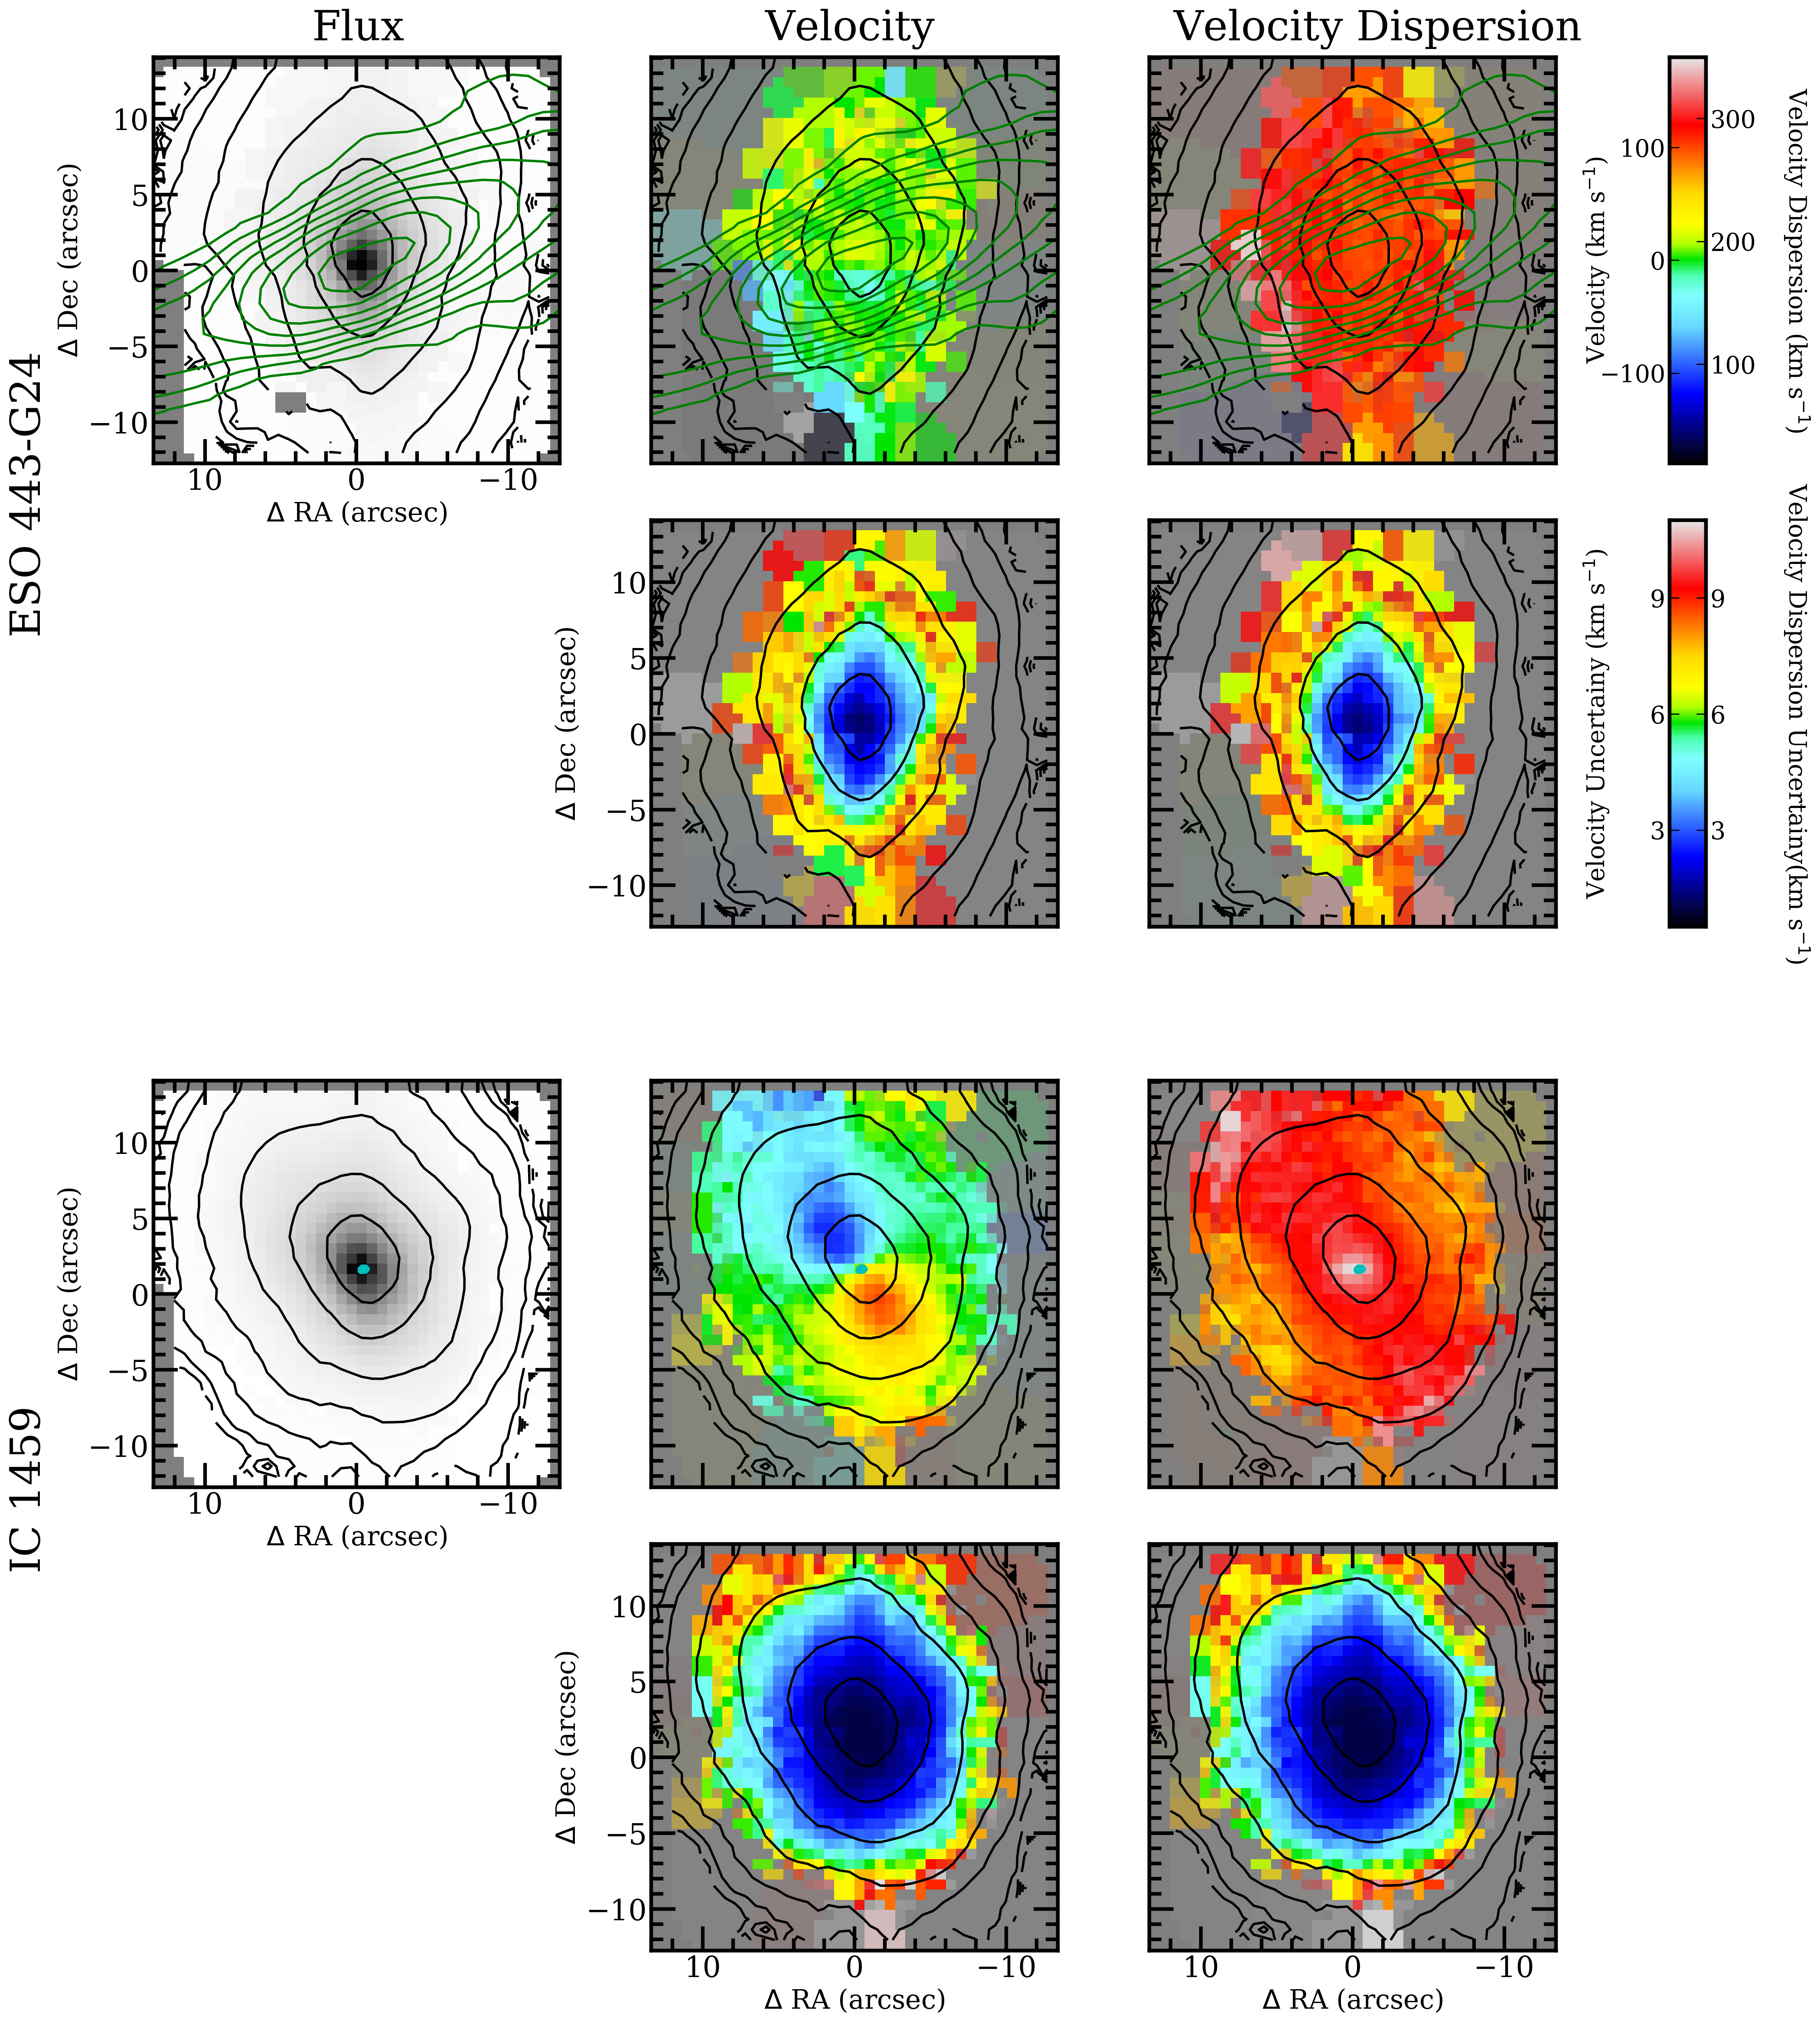
\includegraphics[height=0.94\textheight]{chapter4/vimos/kin1.png}
			\caption[VIMOS stellar kinematic maps]{VIMOS stellar kinematic maps: From left to right: flux (image), velocity and velocity dispersion. Top to bottom: ESO 443-G24, IC 1459 and IC 1531. Rows show parameter and uncertainty in the parameter on alternate rows. Flux contours are shown in black, CO from ALMA in cyan and radio from VLA in red. The radio band displayed depends on the data available in the archive and which images had a similar resolution and and scales}
			\label{fig:VIMOS_stellar}
		\end{figure*}
		\begin{figure*}
			\centering
			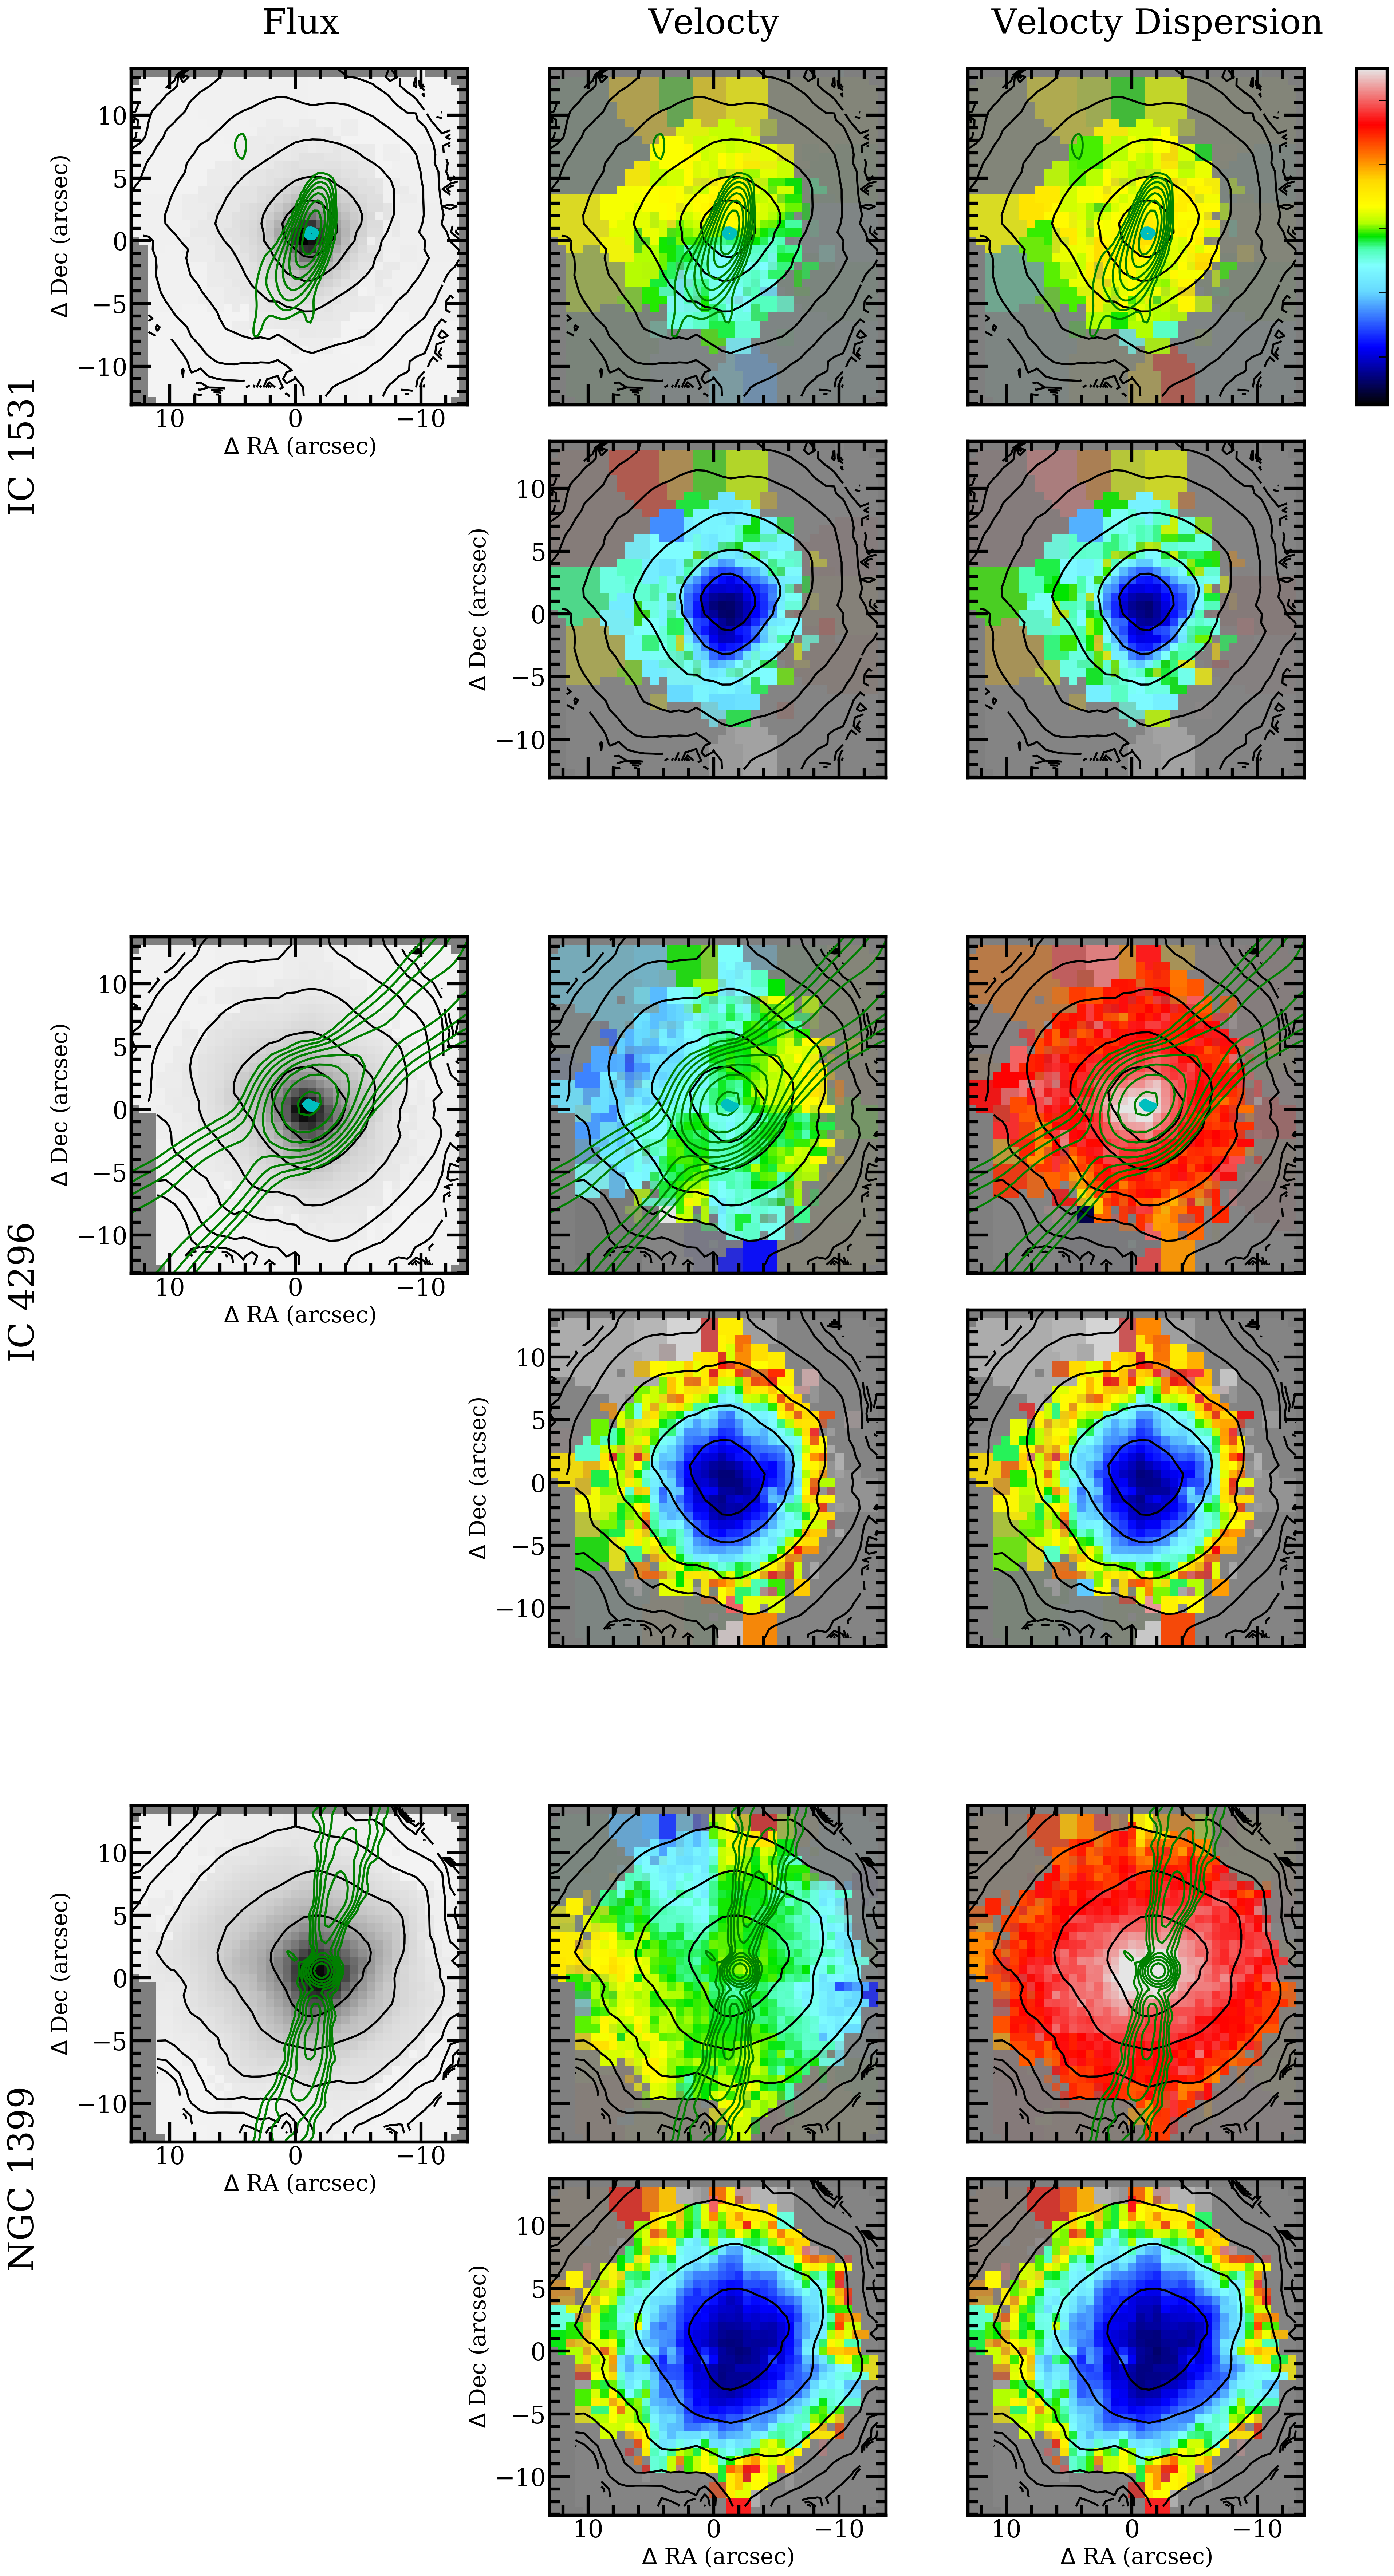
\includegraphics[height=0.94\textheight]{chapter4/vimos/kin2.png}
			\contcaption{continued for IC 4296, NGC 612 and NGC 1399}
		\end{figure*}
		\begin{figure*}
			\centering
			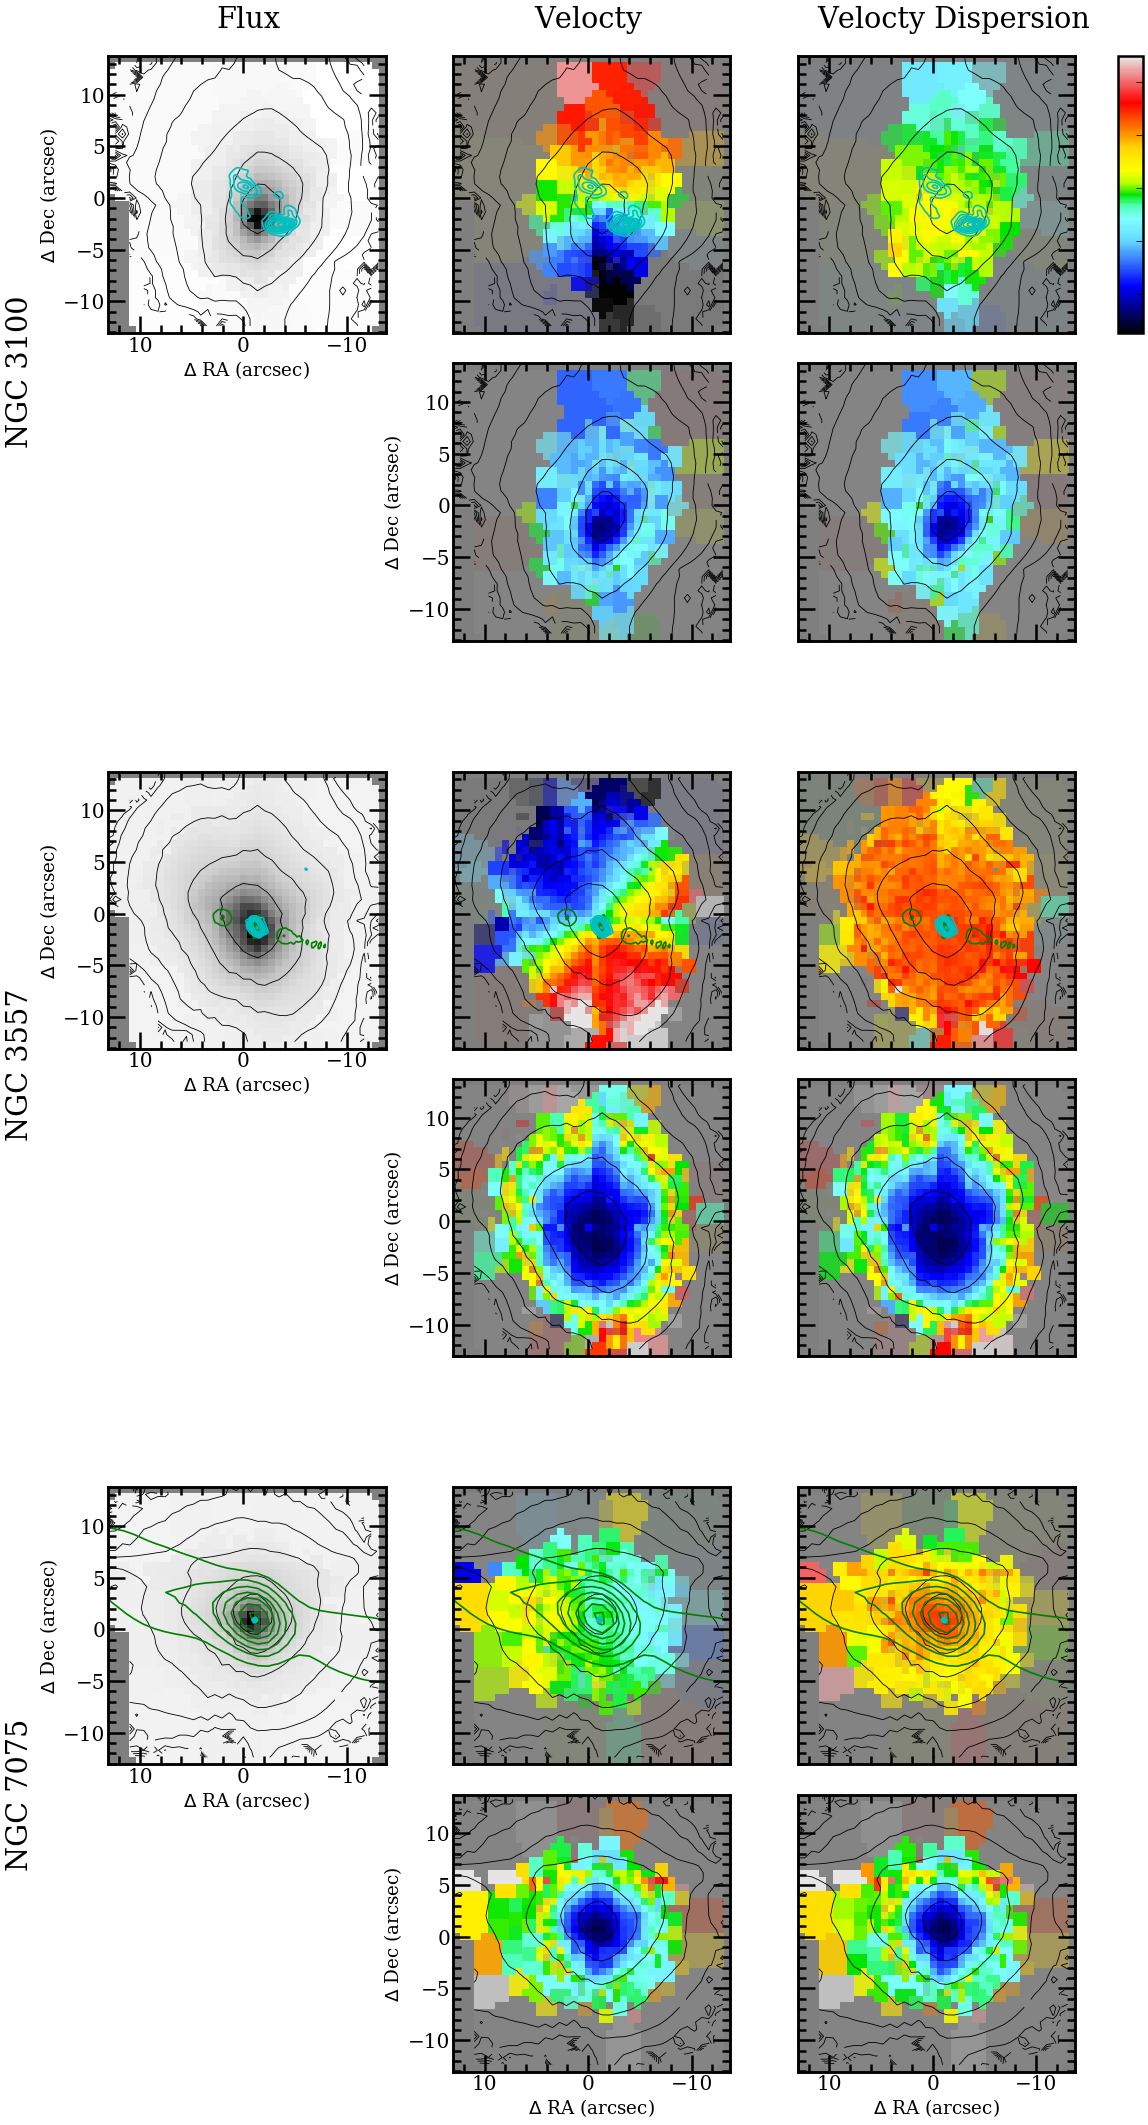
\includegraphics[height=0.94\textheight]{chapter4/vimos/kin3.png}
			\contcaption{continued for NGC 3100, NGC 3557 and NGC 7075}
		\end{figure*}
		\begin{figure*}
			\centering
			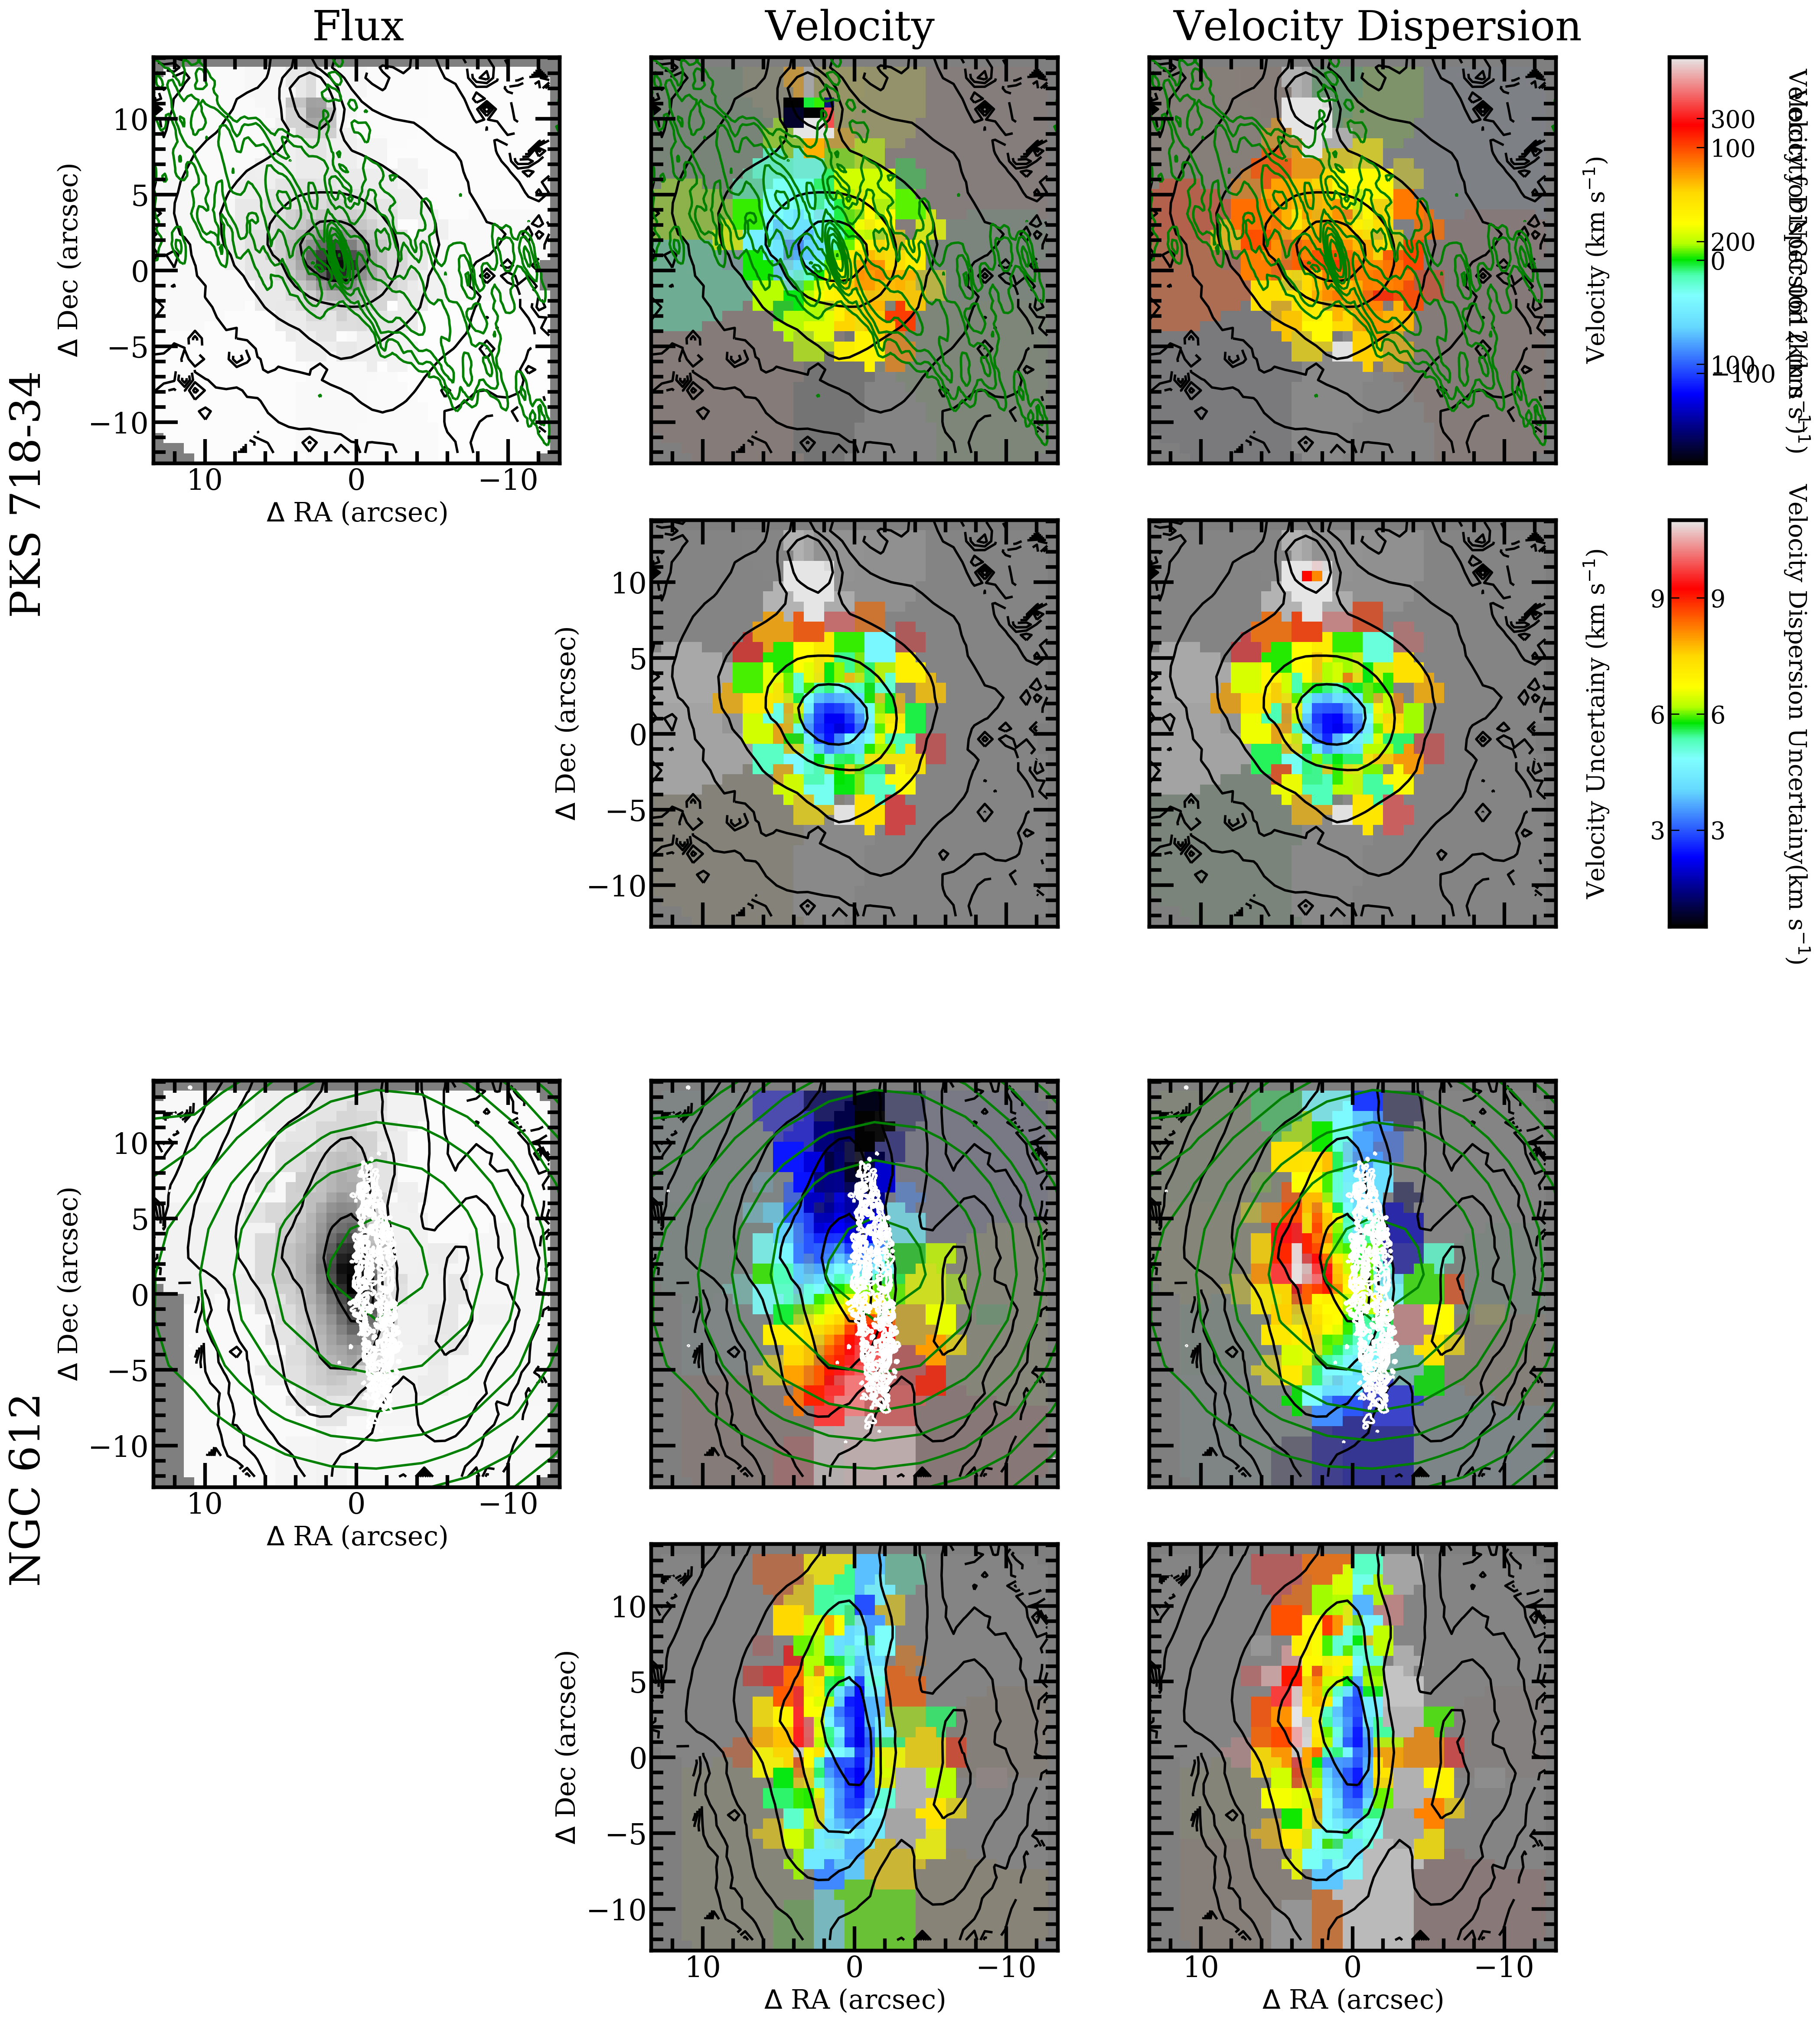
\includegraphics[height=0.31\textheight]{chapter4/vimos/kin4.png}
			\contcaption{continued for PKS 718-34}
		\end{figure*}


		\begin{figure*}
			\centering
			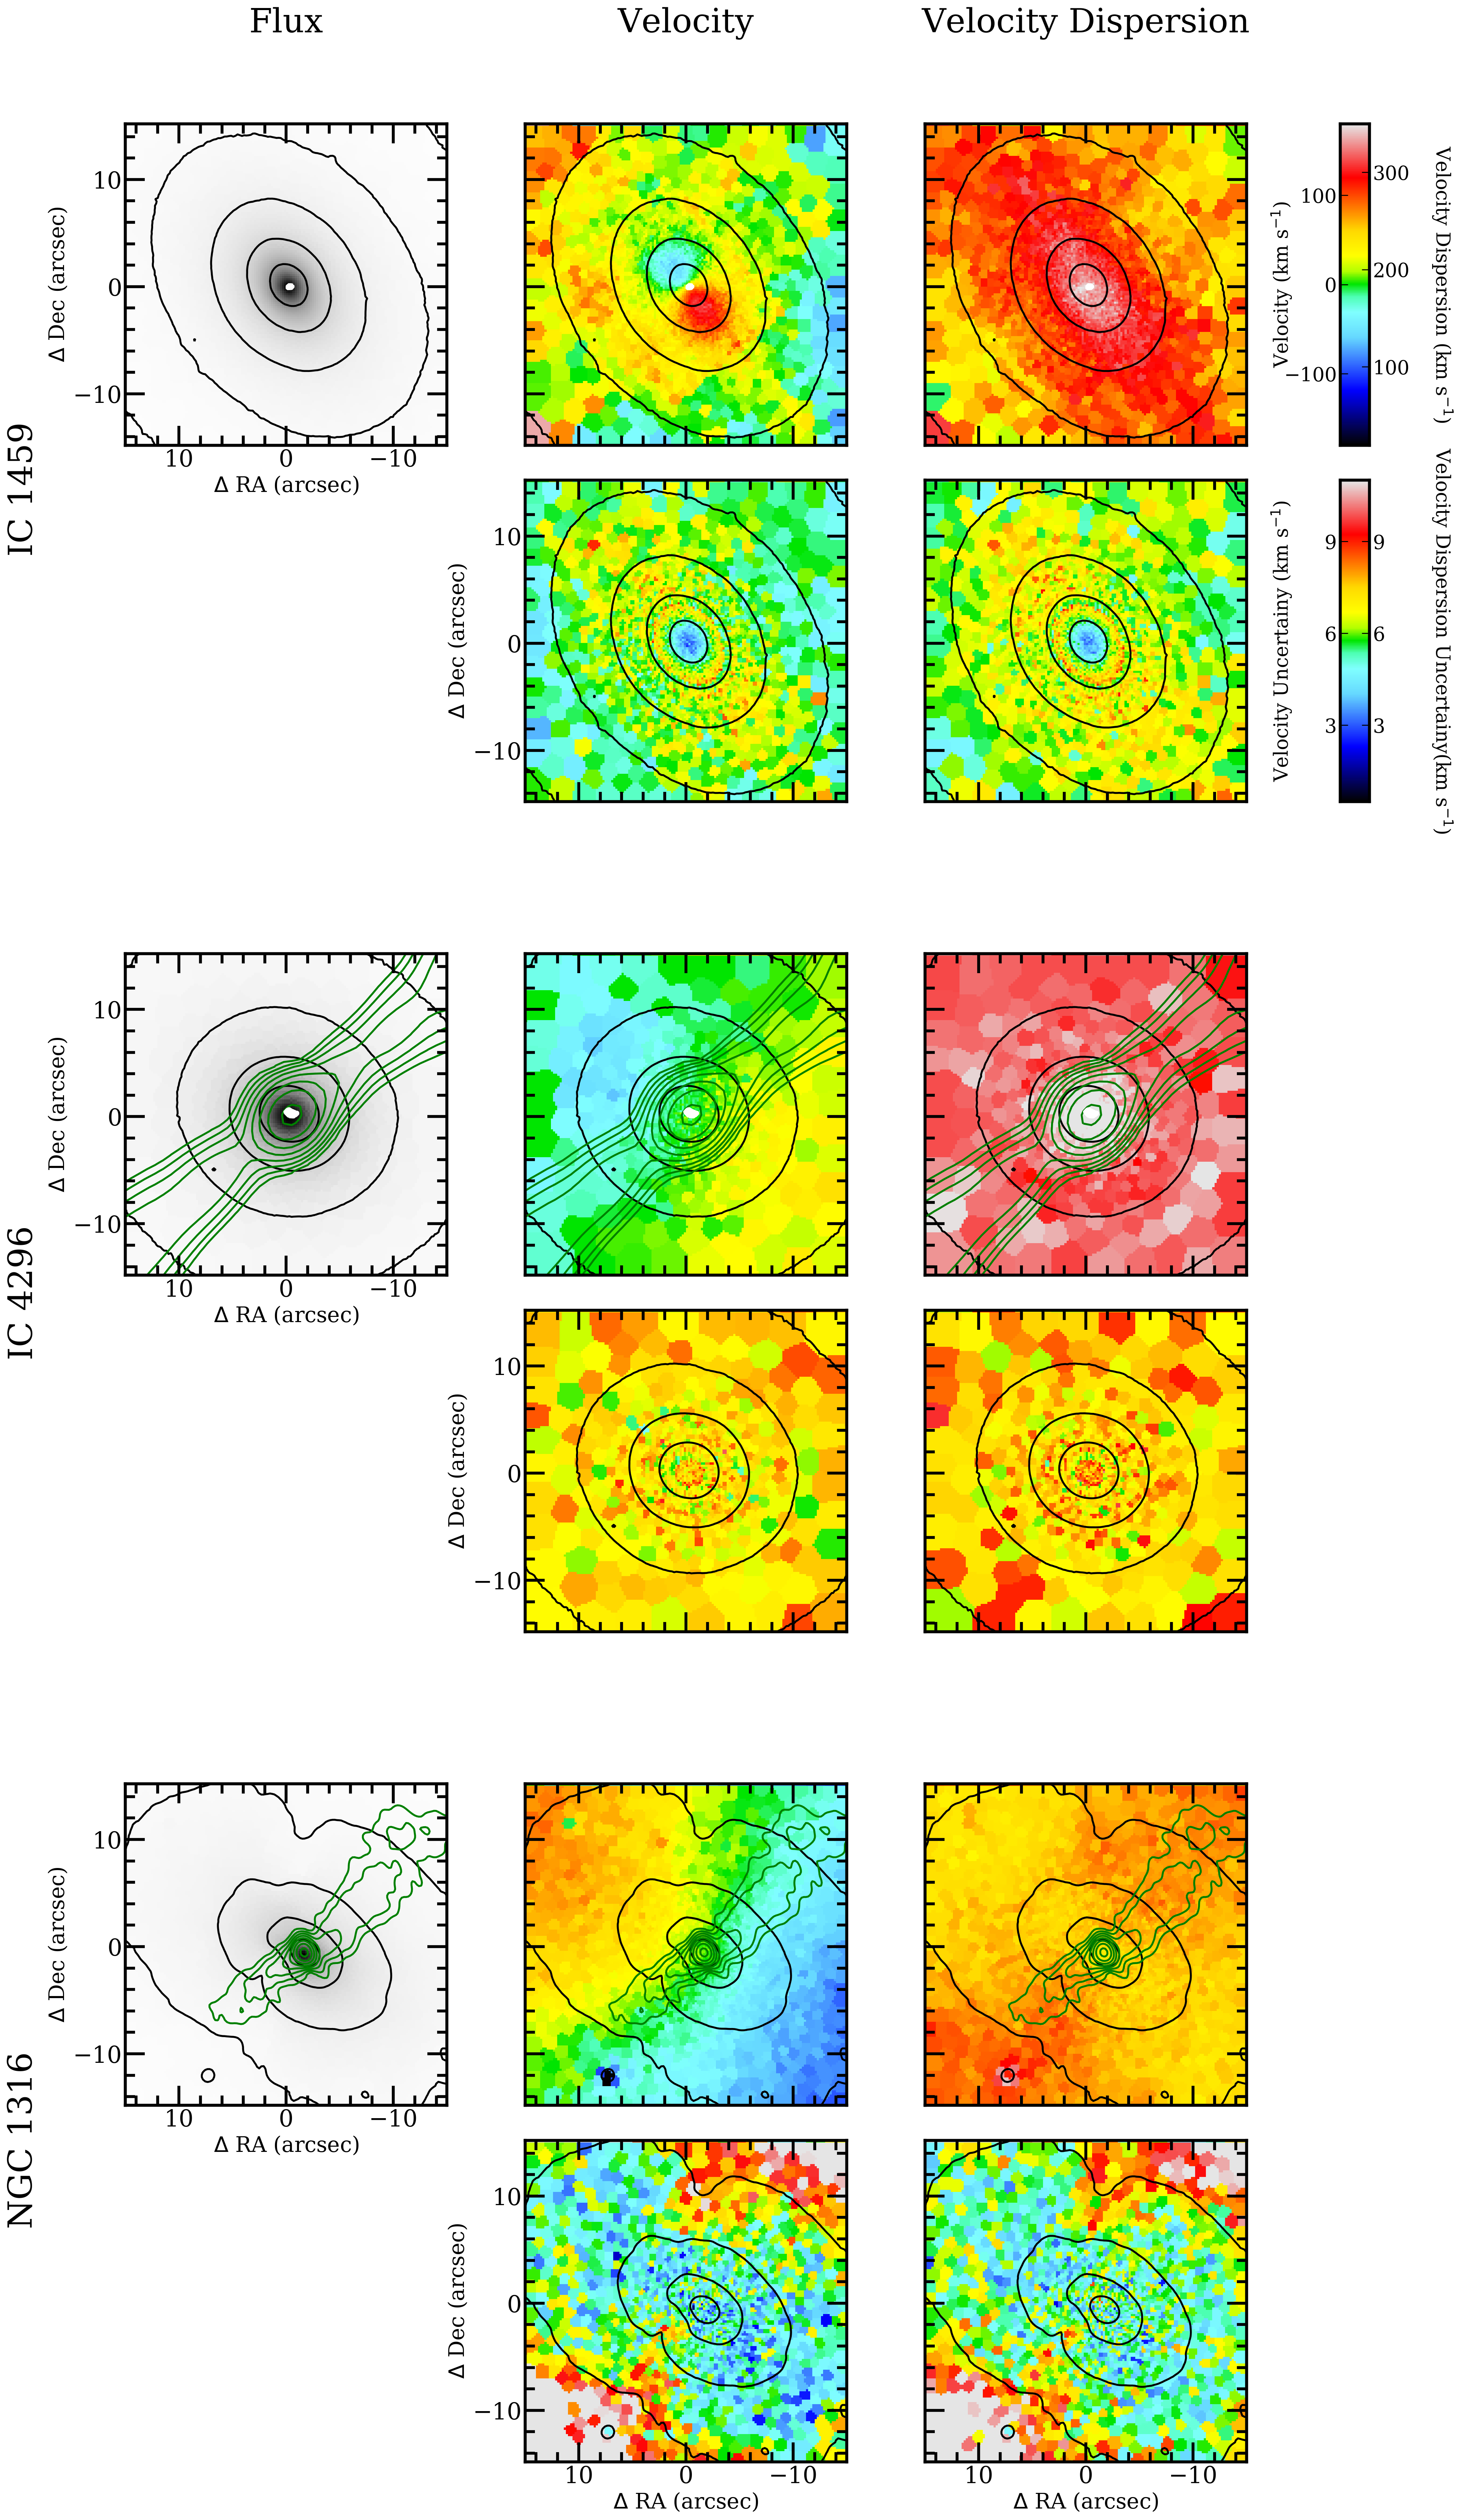
\includegraphics[height=0.94\textheight]{chapter4/muse/kin1.png}
			\caption[MUSE stellar kinematic maps]{MUSE stellar kinematic maps: From top to bottom: IC 1459, IC 4296 and NGC 1316. Plots are as in \ref{fig:VIMOS_absorption}}
			\label{fig:VIMOS_stellar}
		\end{figure*}
		\begin{figure*}
			\centering
			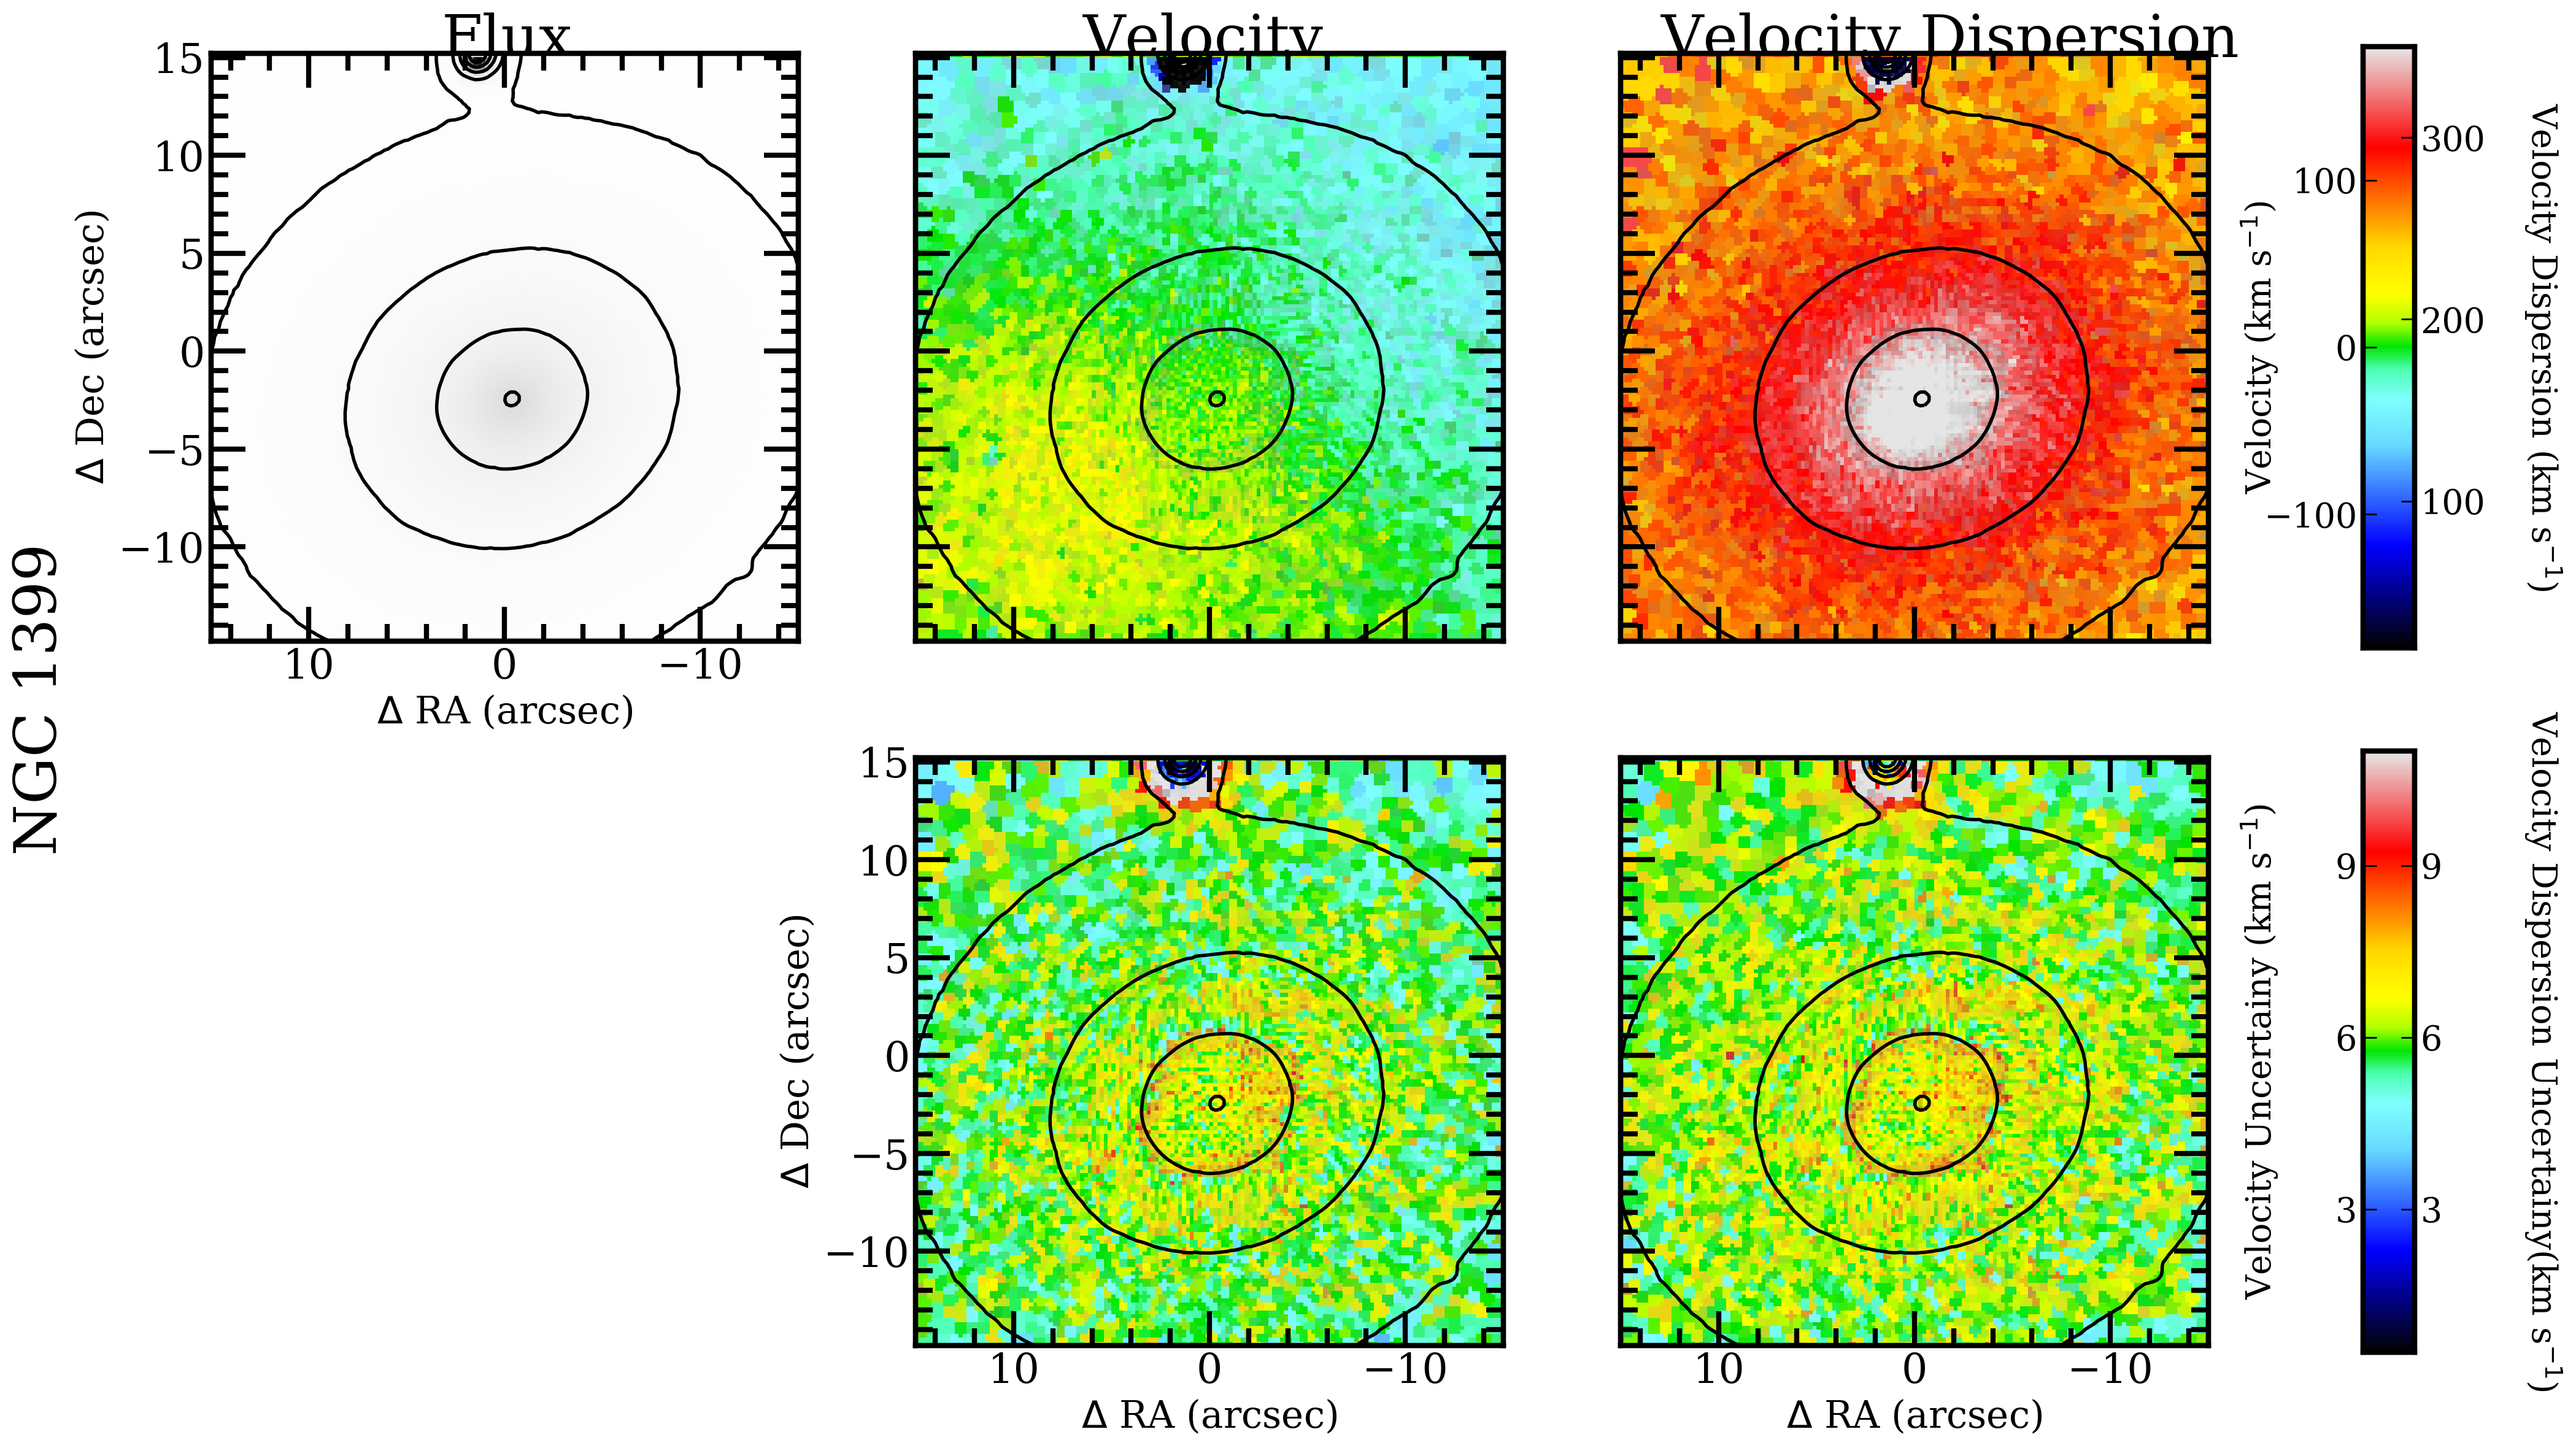
\includegraphics[height=0.31\textheight]{chapter4/muse/kin2.png}
			\contcaption{continued for NGC 1399}
		\end{figure*}

		
		The kinematics of the sample are classified according to the Regular-Rotator/Non Regular-Rotator (RR/NRR) regime given in \citet{Krajnovic2011}, Fast/Slow Rotator (FR/SR) regime given in \citet{Cappellari2016} (originally defined by \citet{Emsellem2011}, but later refined by \citet{Cappellari2016}). This classification is shown on the $\lambda_{R_e}$--ellipticity plane in figure \ref{fig:lambdaR_ellip}. Beyond this attempts have been made to use the kinematic features as defined in \citet{Krajnovic2011} in a algorithmic way, however the quality of the data has meant that many have had to be classified by eye as the artifacts from the VIMOS quadrants confuse any ellipse fitting methods. These classifications are given in table \ref{tab:classify}. 


		\begin{table}
			\centering
			\caption{Kinematic classifications. Where we have MUSE datacubes, the value and classifications from this are given (since they rely on less extrapolation due to the larger field of view of MUSE), otherwise the values are from the VIMOS maps. Col. 1: Galaxy name, Col. 2: $\lambda_{R_e}$, Col. 3: ellipticity, Col. 4: Misalignment between kinematic position angle and photometric position angle, Col. 5: Fast or Slow rotator, Col. 6: Regular rotator or non-regular rotator, Col. 7: Kinematic features (abbreviations defined in section \ref{sec:ETG}), Col. 8: Kinematic group as defined in section \ref{sec:ETG}}
			\label{tab:classify}
			\begin{tabular}{l r r p{0.7cm} l l l l}
				\hline
				\hline
				Galaxy		& $\lambda_{R_e}$ & $\epsilon$  & $\Gamma_\text{kin}$ (deg) & FR/ SR 	& RR/ NRR 	& Feat. & Group 	\\
				\hline 
				ESO 443-G024 & 0.031 & 0.32 & 55.2 	& FR & NRR & KDC & c \\
				IC 1459 	& 0.174 & 0.24 & 87.9	& SR & NRR & KDC & c \\
				IC 1531 	& 0.100 & 0.11 & 64.4 	& SR & NRR & LV & a \\
				IC 4296		& 0.034 & 0.03 & 83.2 	& SR & RR & -- & e \\
				NGC 612 	& 0.519 & 0.58 & 7.3 	& FR & RR & -- & e \\
				NGC 1316 	& 0.100 & 0.39 & 72.1 	& FR & NRR & -- & f \\
				NGC 1399 	& 0.090 & 0.12 & 27.2 	& SR & NRR & LV & a \\
				NGC 3100 	& 0.418 & 0.31 & 19.8 	& FR & RR & -- & e \\
				NGC 3557 	& 0.320 & 0.22 & 7.6 	& FR & RR & -- & e\\
				NGC 7075 	& 0.048 & 0.09 & 20.0 	& SR & NRR & -- & b \\
				PKS 718-34  & 0.152 & 0.18 & 57.7 	& SR & NRR & KDC$^\text{a}$ & b\\
				\hline
				\hline
				\multicolumn{7}{L{.9\textwidth}}{\footnotesize $^\text{a}$ This is a tentative classification. Higher S/N is required to a larger radii to confirm this.} \\ % need to adjust size for final table
			\end{tabular}
		\end{table}

		Column 4 in table \ref{tab:classify} shows the misalignment between the photometric position angle and the kinematic position angle ($\Gamma_\text{kin} = \left| \mathrm{PA_{phot}} - \mathrm{PA_{kin}} \right|$). \citet{Cappellari2007, Krajnovic2011, Fogarty2015} showed that regular rotating galaxies almost always have have aligned kinematic and photometric axes (with a scatter of just 4\degree). Regular rotators with a significant misalignment are either very round, interacting or strongly barred. Taking into account the lower quality of data our results are consistent with this: of the 4 regular rotating galaxies in the Southern sample, 2 are misaligned to less than 8\degree and the other 2 are round (one of which is extremely round). As noted in \citet{Cappellari2016} this result requires that regular rotators are axis-symmetric. 

		Misalignments are routinely observed for non-regularly rotating galaxies, which our observations are also consistent with. This generally implies a more triaxial intrinsic shape, however large misalignments are extremely rarely observed in galaxies with $\epsilon > 0.4$ suggesting that non-regularly rotating galaxies are more spherical in shape. This is the reason for the $\epsilon < 0.4$ requirement in the definition for slow rotators. 


	\subsection{Fast/Slow Rotator fraction}
		\label{subsec:FSfrac}
		The radial $\lambda_{R_e}$ profiles are shown in figure \ref{fig:lambdaR_profile}. The huge jump in $\lambda_{R_e}$ in one of the MUSE profiles is due to a foreground star in the NGC 1316 field of view. 

		Using the combined samples of Atlas3D and MASSIVE, we find that there is no discernible difference between the radio selected Southern Sample and the optically selected ETGs of Atlas3D and MASSIVE, once the differences in mass distribution are taken into account. To do this we find the fraction of slow rotators in each mass bin (using $M_k$ as a proxy), shown in black in the lower panel of figure \ref{fig:SRmassFraction}. We using this and the distribution in mass of the Southern Sample (red in upper panel of \ref{fig:SRmassFraction}) to estimate that we should expect $(64 \pm 6)\%$ of the Southern Sample to be slow rotators. This is consistent with out finding of 56\% slow rotators.

		\begin{figure}
			\centering
			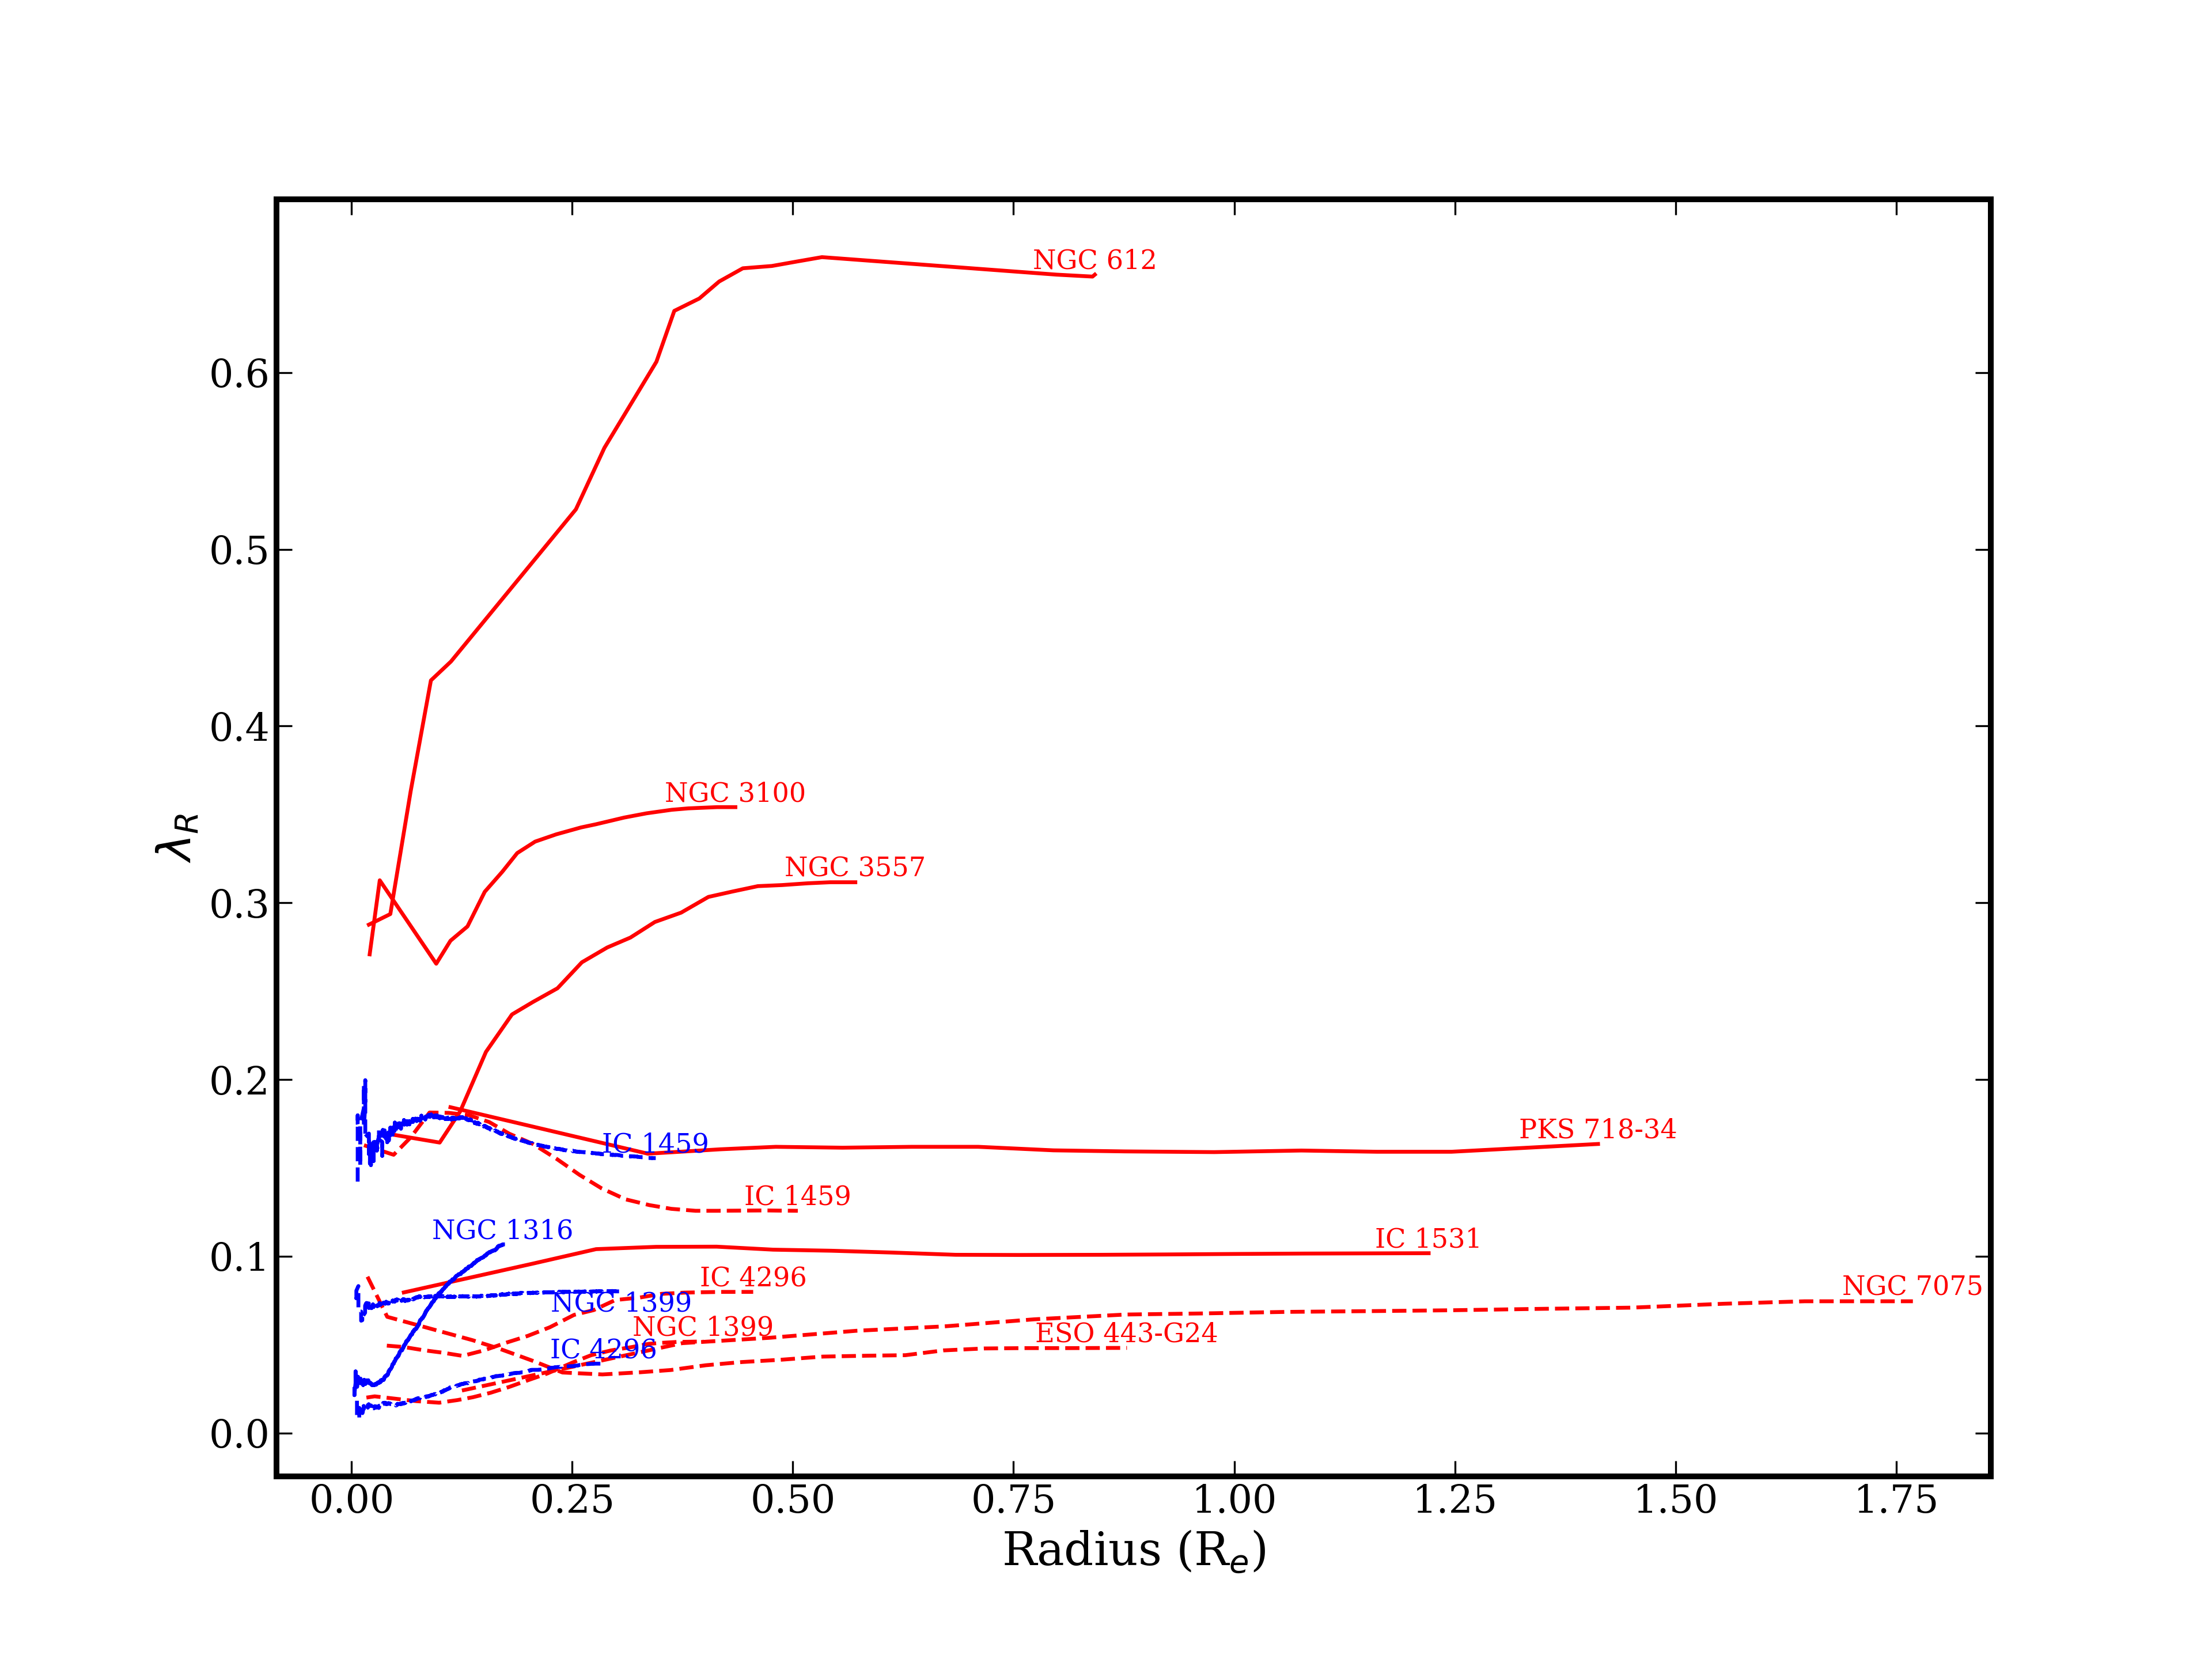
\includegraphics[width=\textwidth]{chapter4/lambda_R.png}
			\caption[$\lambda_{R}$ radial profiles]{The radial $\lambda_{R}$ profiles. Profiles from VIMOS data are in red, while MUSE data is in red. Solid lines represent fast rotators, while dashed represents slow rotators.}
			\label{fig:lambdaR_profile}
		\end{figure}


		\begin{figure}
			\centering
			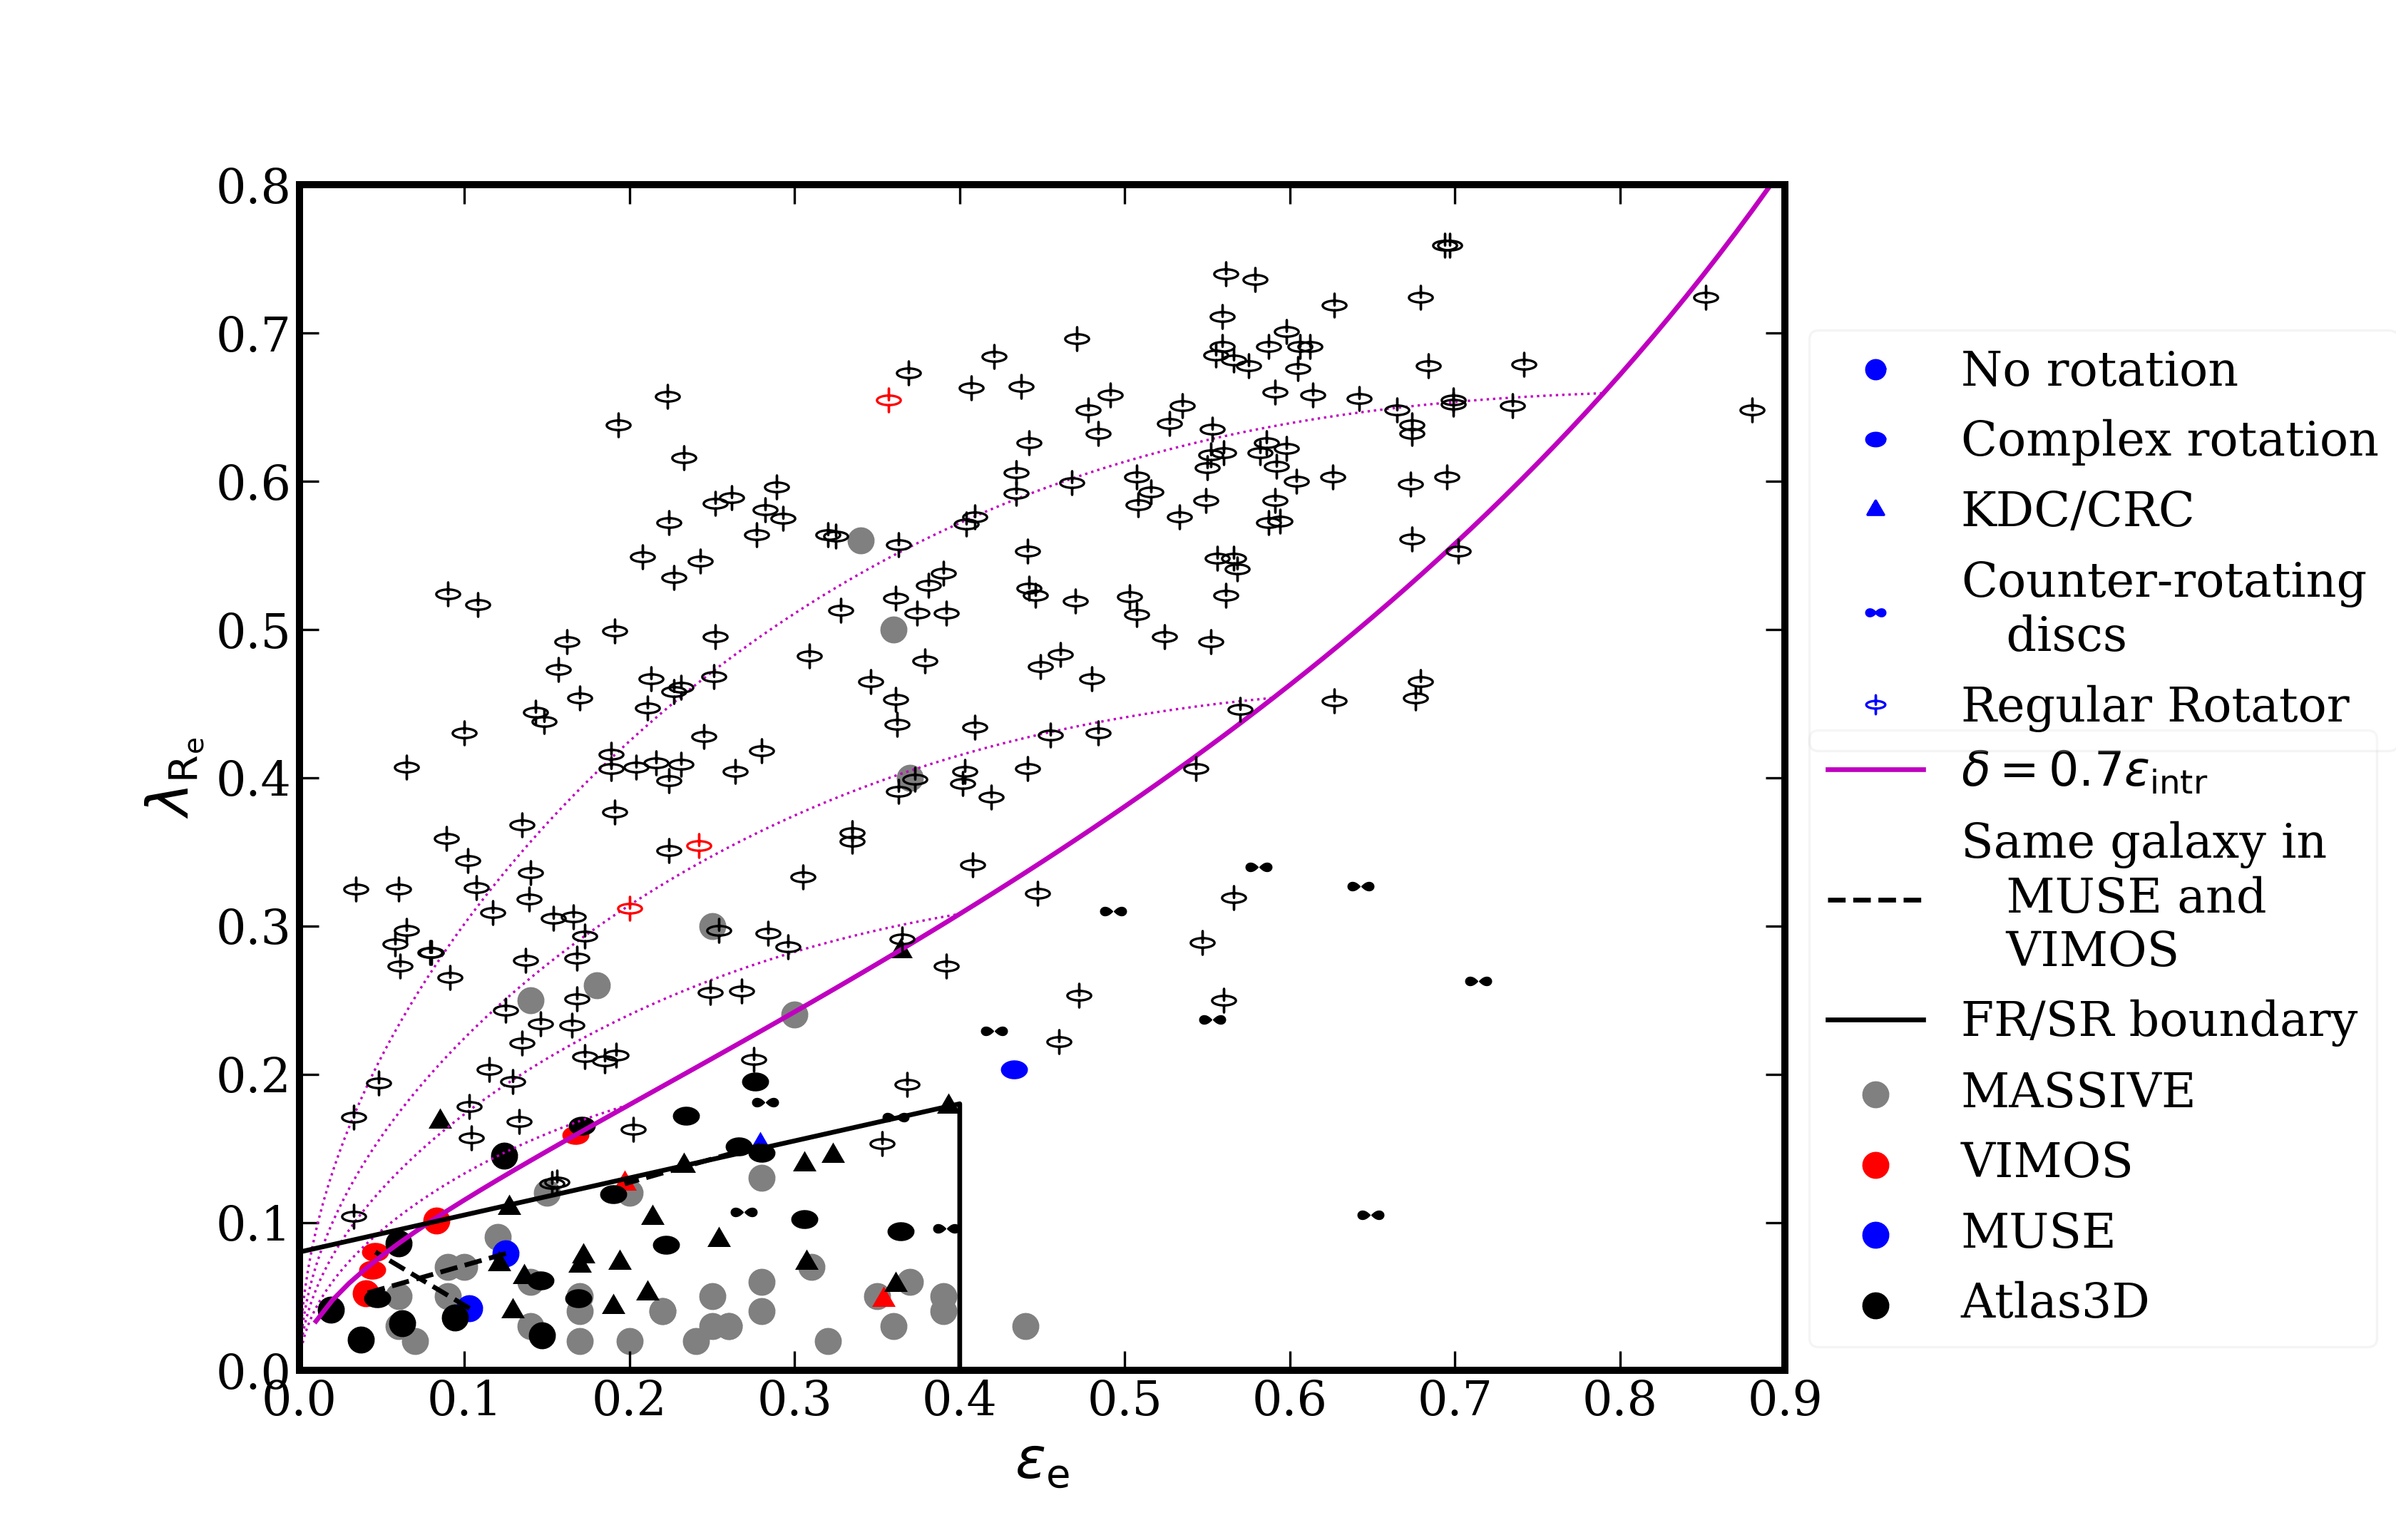
\includegraphics[width=\textwidth]{chapter4/lambda_R_ellipticity.png}
			\caption[$\lambda_{R_e}$ -- ellipticity plane]{The $\lambda_{R_e}$ -- ellipticity plane showing the definition for the fast/slow rotator classes (solid black line). Atlas3D galaxies are shown in black \citep{Emsellem2011} and MASSIVE survey galaxies are shown in gray \citep{Veale2017}. The theoretic limit of disk dominated galaxy is shown (solid magenta) with lines of constant intrinsic angular moment with varying inclination (dashed magenta). VIMOS and MUSE measurements are shown in red and blue respectively. Note: the MASSIVE survey does not classify substructure so the MASSIVE sample is simply shown with filled circles.}
			\label{fig:lambdaR_ellip}
		\end{figure}


		

		\begin{figure}
			\centering
			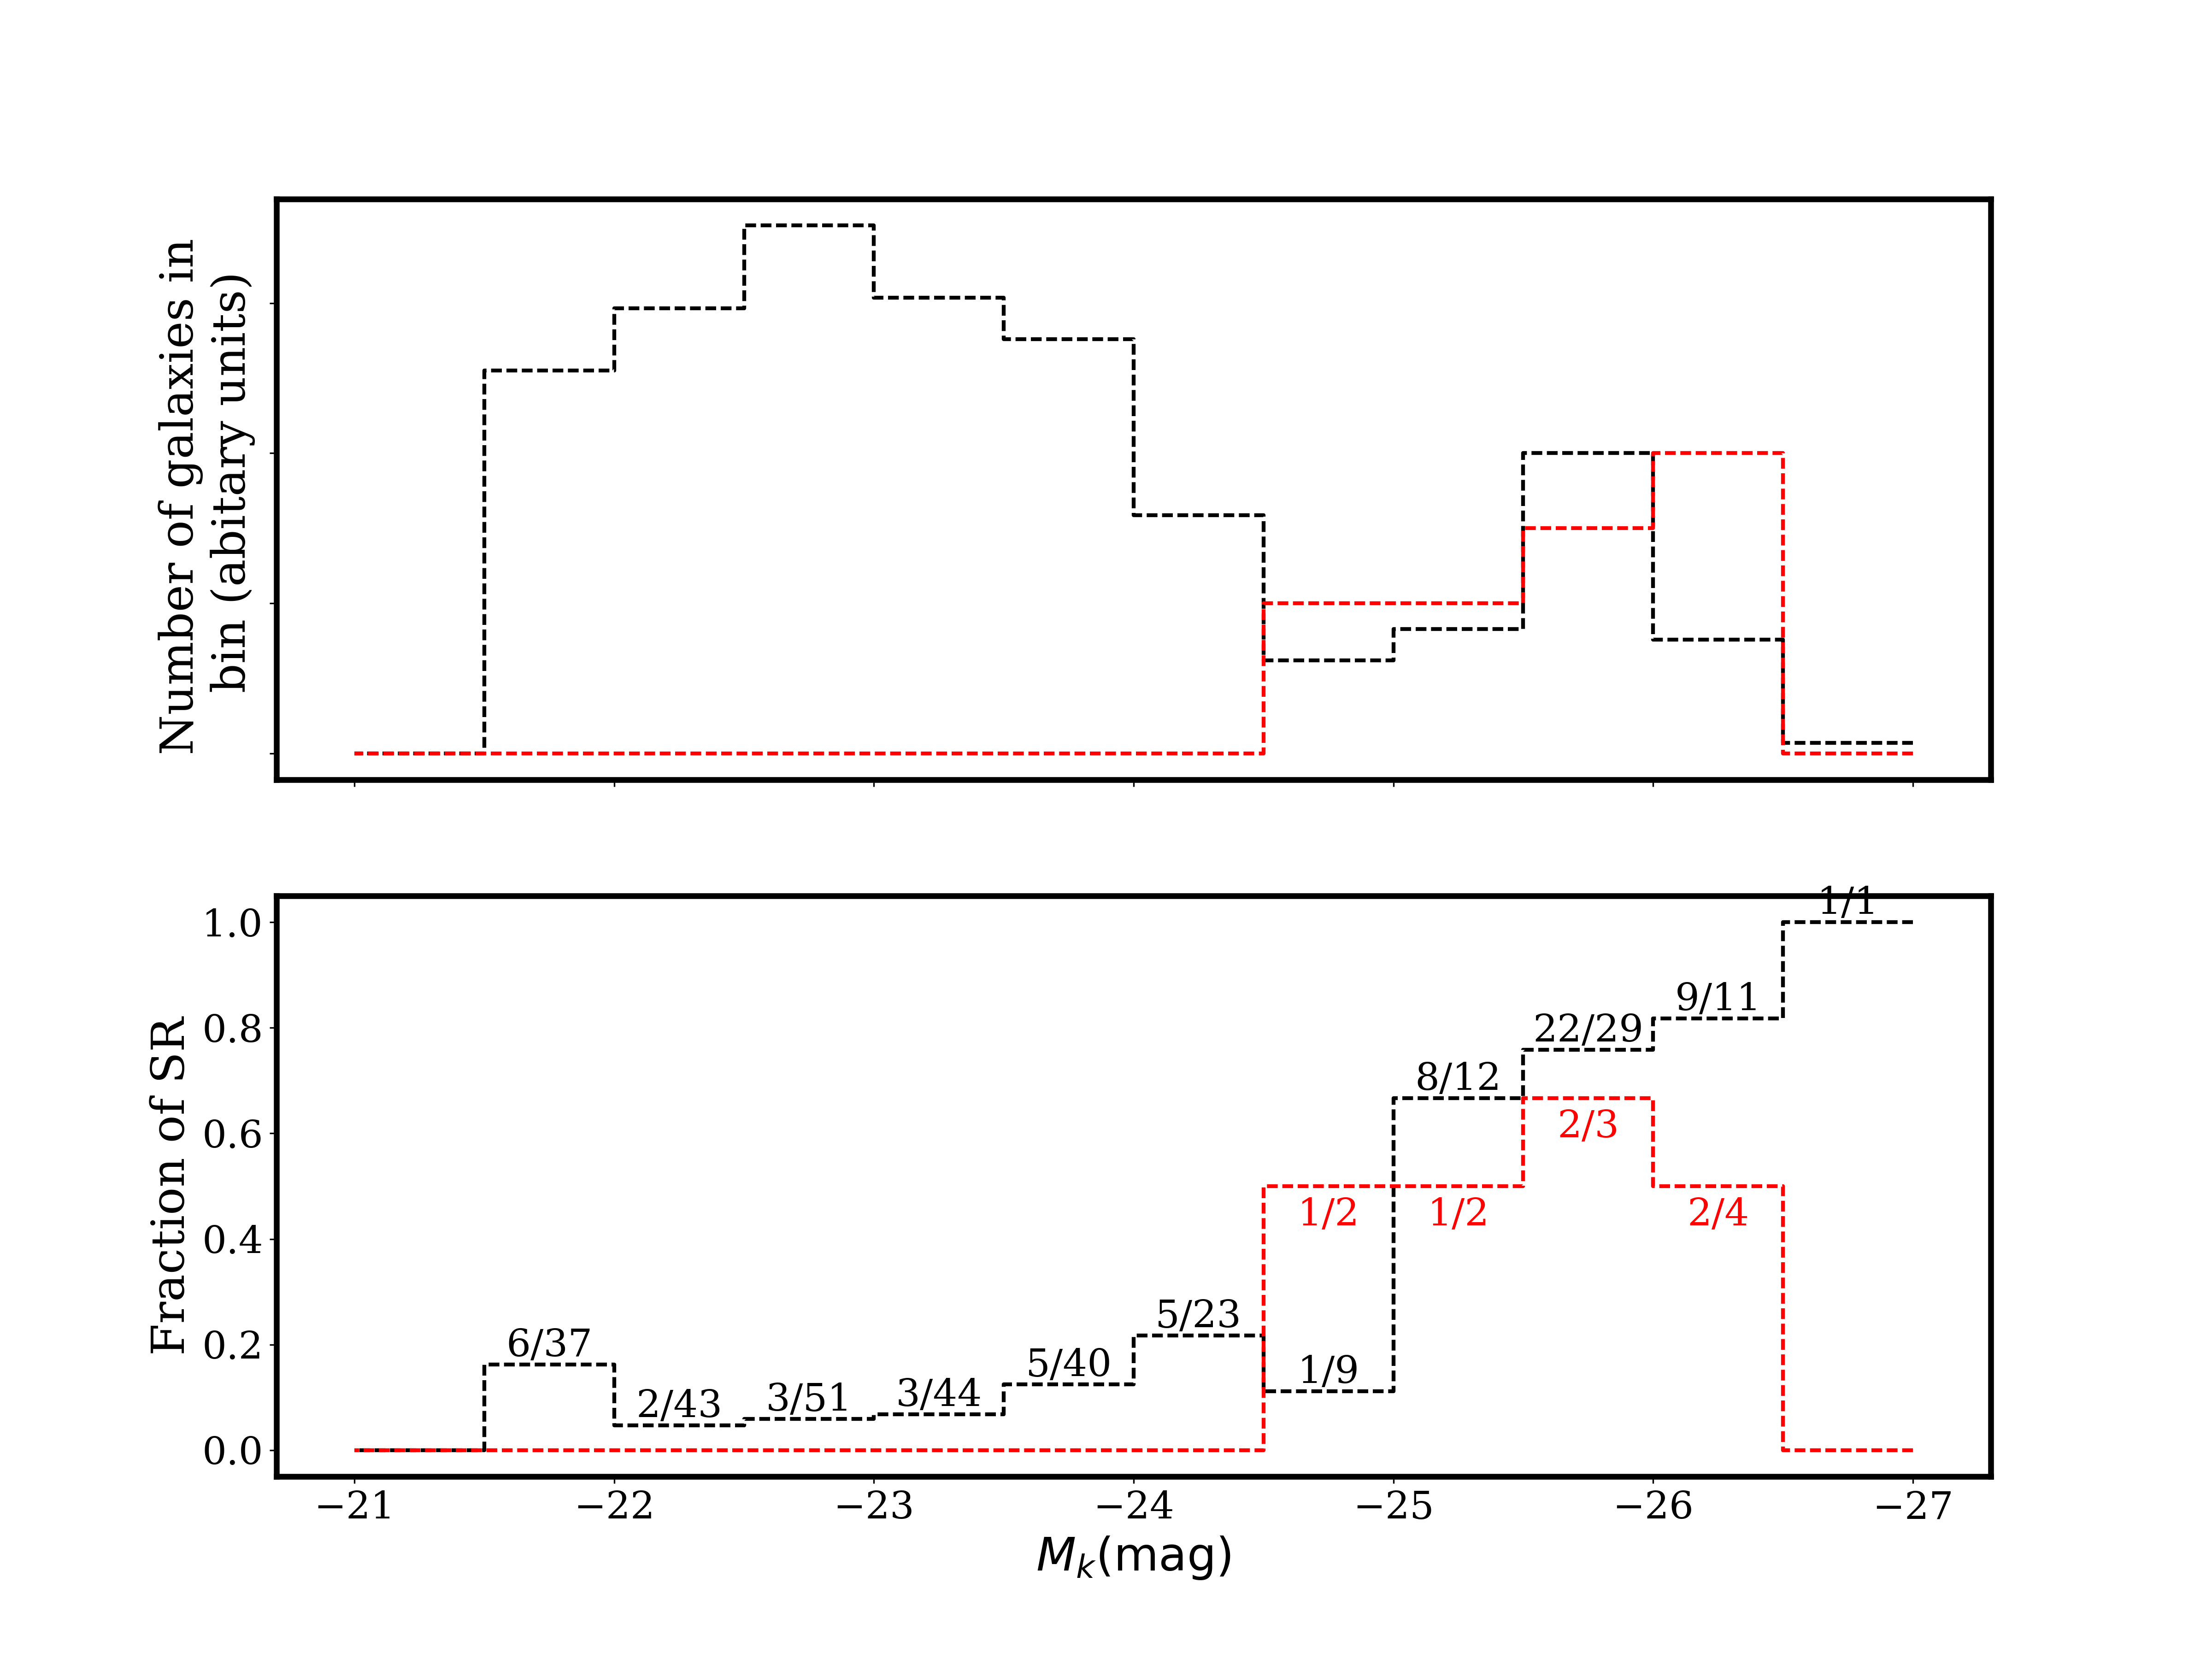
\includegraphics[width=\textwidth]{chapter4/M_k_binned.png}
			\caption[Mass matching global kinematics]{The mass distributions (upper panel) of the combined Atlas3D and MASSIVE surveys (black) and the Southern Sample (red), as well as the slow rotators fractions within each mass bin (lower panel). The labels display the [number of slow rotators]/[total number of galaxies] in that bin. Note that the black and red have different normalizations in the mass distribution plot: The combined Atlas3D and MASSIVE samples contains 300 galaxies, while the Southern Sample is just 11 radio galaxies.}
			\label{fig:SRmassFraction}
		\end{figure}


		





\section{Stellar Population}
	\label{sec:pop}

	\subsection{Absorption line strengths}
		\label{subsec:absorption}
		Figures \ref{fig:VIMOS_absorption} and \ref{fig:MUSE_absorption} show the resolved absorption line strengths for the Southern Sample. For the VIMOS cubes, we find G4300, Fe4383, Ca4455, Fe4531, H$_\beta$, Fe5015 and Mg$_b$. For the most distant galaxies, the continuum band for Mg$_b$ is redshifted beyond the range of the VIMOS spectrograph. In these cases, we have avoided unnecessary systematics, by not calculating Mg$_b$. For MUSE cubes, we find H$_\beta$, Fe5015, Mg$_b$, Fe5270, Fe5335, Fe5406, Fe5709, Fe5782, NaD, TiO1 and TiO2. Each index is defined in table \ref{tab:abIndex}. 

		\begin{table}
			\centering
			\caption{The definitions used for each index. Indices are from \citet{Trager1998}.}
			\label{tab:abIndex}
			\begin{tabular}{l c c c}
				\hline
				\hline
				Index 	& Blue cont. 		& Index band 		& Red cont. \\
				\hline 
				G4300 	& 4266.375--4282.625 & 4281.375--4316.375 & 4318.875--4335.125 \\
				Fe4383 	& 4359.125--4370.375 & 4369.125--4420.375 & 4442.875--4455.375 \\
				Ca4455 	& 4445.875--4454.625 & 4452.125--4474.625 & 4477.125--4492.125 \\
				Fe4531 	& 4504.250--4514.250 & 4514.250--4559.250 & 4560.500--4579.250 \\
				H$_\beta$ & 4827.875--4847.875 & 4847.875--4876.625 & 4876.625--4891.625 \\
				Fe5015 	& 4946.500--4977.750 & 4977.750--5054.000 & 5054.000--5065.250 \\
				Mg$_b$ 	& 5142.625--5161.375 & 5160.125--5192.625 & 5191.375--5206.375 \\
				Fe5270 	& 5233.150--5248.150 & 5245.650--5285.650 & 5285.650--5318.150 \\
				Fe5335 	& 5304.625--5315.875 & 5312.125--5352.125 & 5353.375--5363.375 \\
				Fe5406 	& 5376.250--5387.500 & 5387.500--5415.000 & 5415.000--5425.000 \\
				Fe5709 	& 5672.875--5696.625 & 5696.625--5720.375 & 5722.875--5736.625 \\
				Fe5782 	& 5765.375--5775.375 & 5776.625--5796.625 & 5797.875--5811.625 \\
				NaD 	& 5860.625--5875.625 & 5876.875--5909.375 & 5922.125--5948.125 \\
				TiO1 	& 5816.625--5849.125 & 5936.625--5994.125 & 6038.625--6103.625 \\
				TiO2 	& 6066.625--6141.625 & 6189.625--6272.125 & 6372.625--6415.125 \\
				\hline
				\hline
			\end{tabular}
		\end{table}

		\begin{figure*}
			\centering
			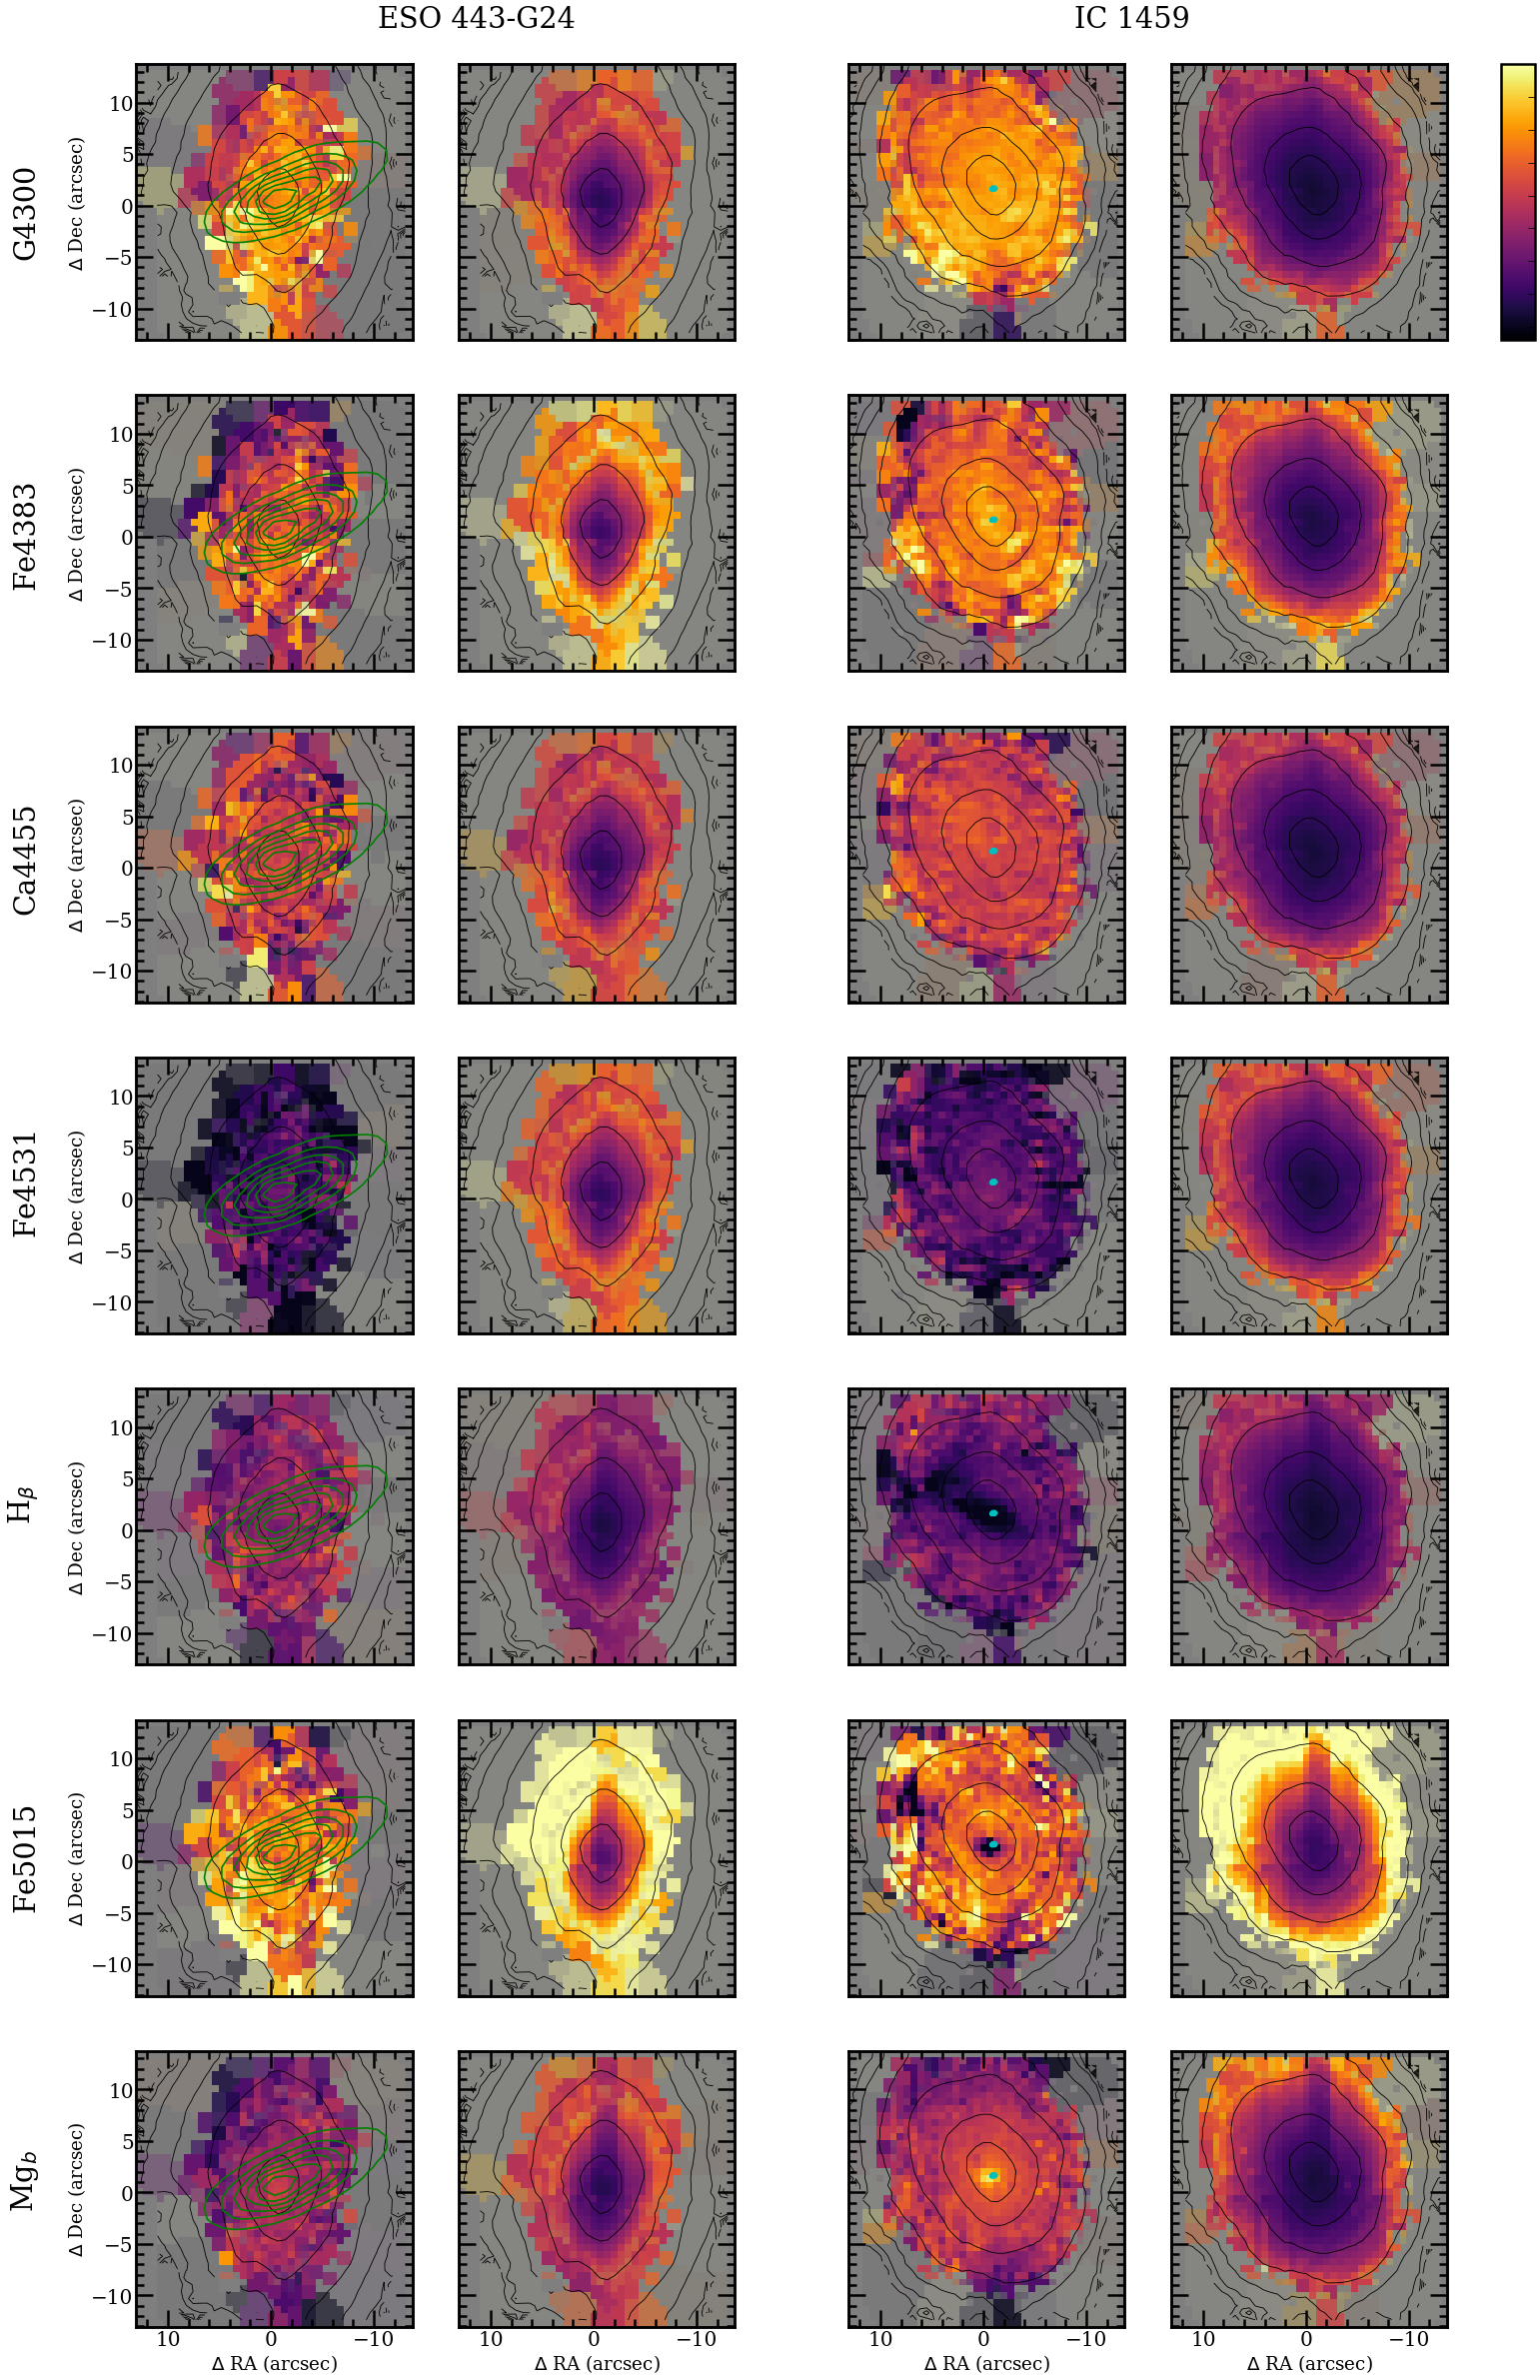
\includegraphics[height=0.94\textheight]{chapter4/vimos/abs1.png}
			\caption[VIMOS absorption line strength maps]{VIMOS stellar kinematic maps: From left to right: ESO 443-G24, ESO 443-G24 uncertainties, IC 1459 and IC 1459 uncertainties. From top to bottom: G4300, Fe4383, Ca4455, Fe4531, H$_\beta$, Fe5015, Mg$_b$. Plots are as in \ref{fig:VIMOS_absorption}}
			\label{fig:VIMOS_absorption}
		\end{figure*}
		\begin{figure*}
			\centering
			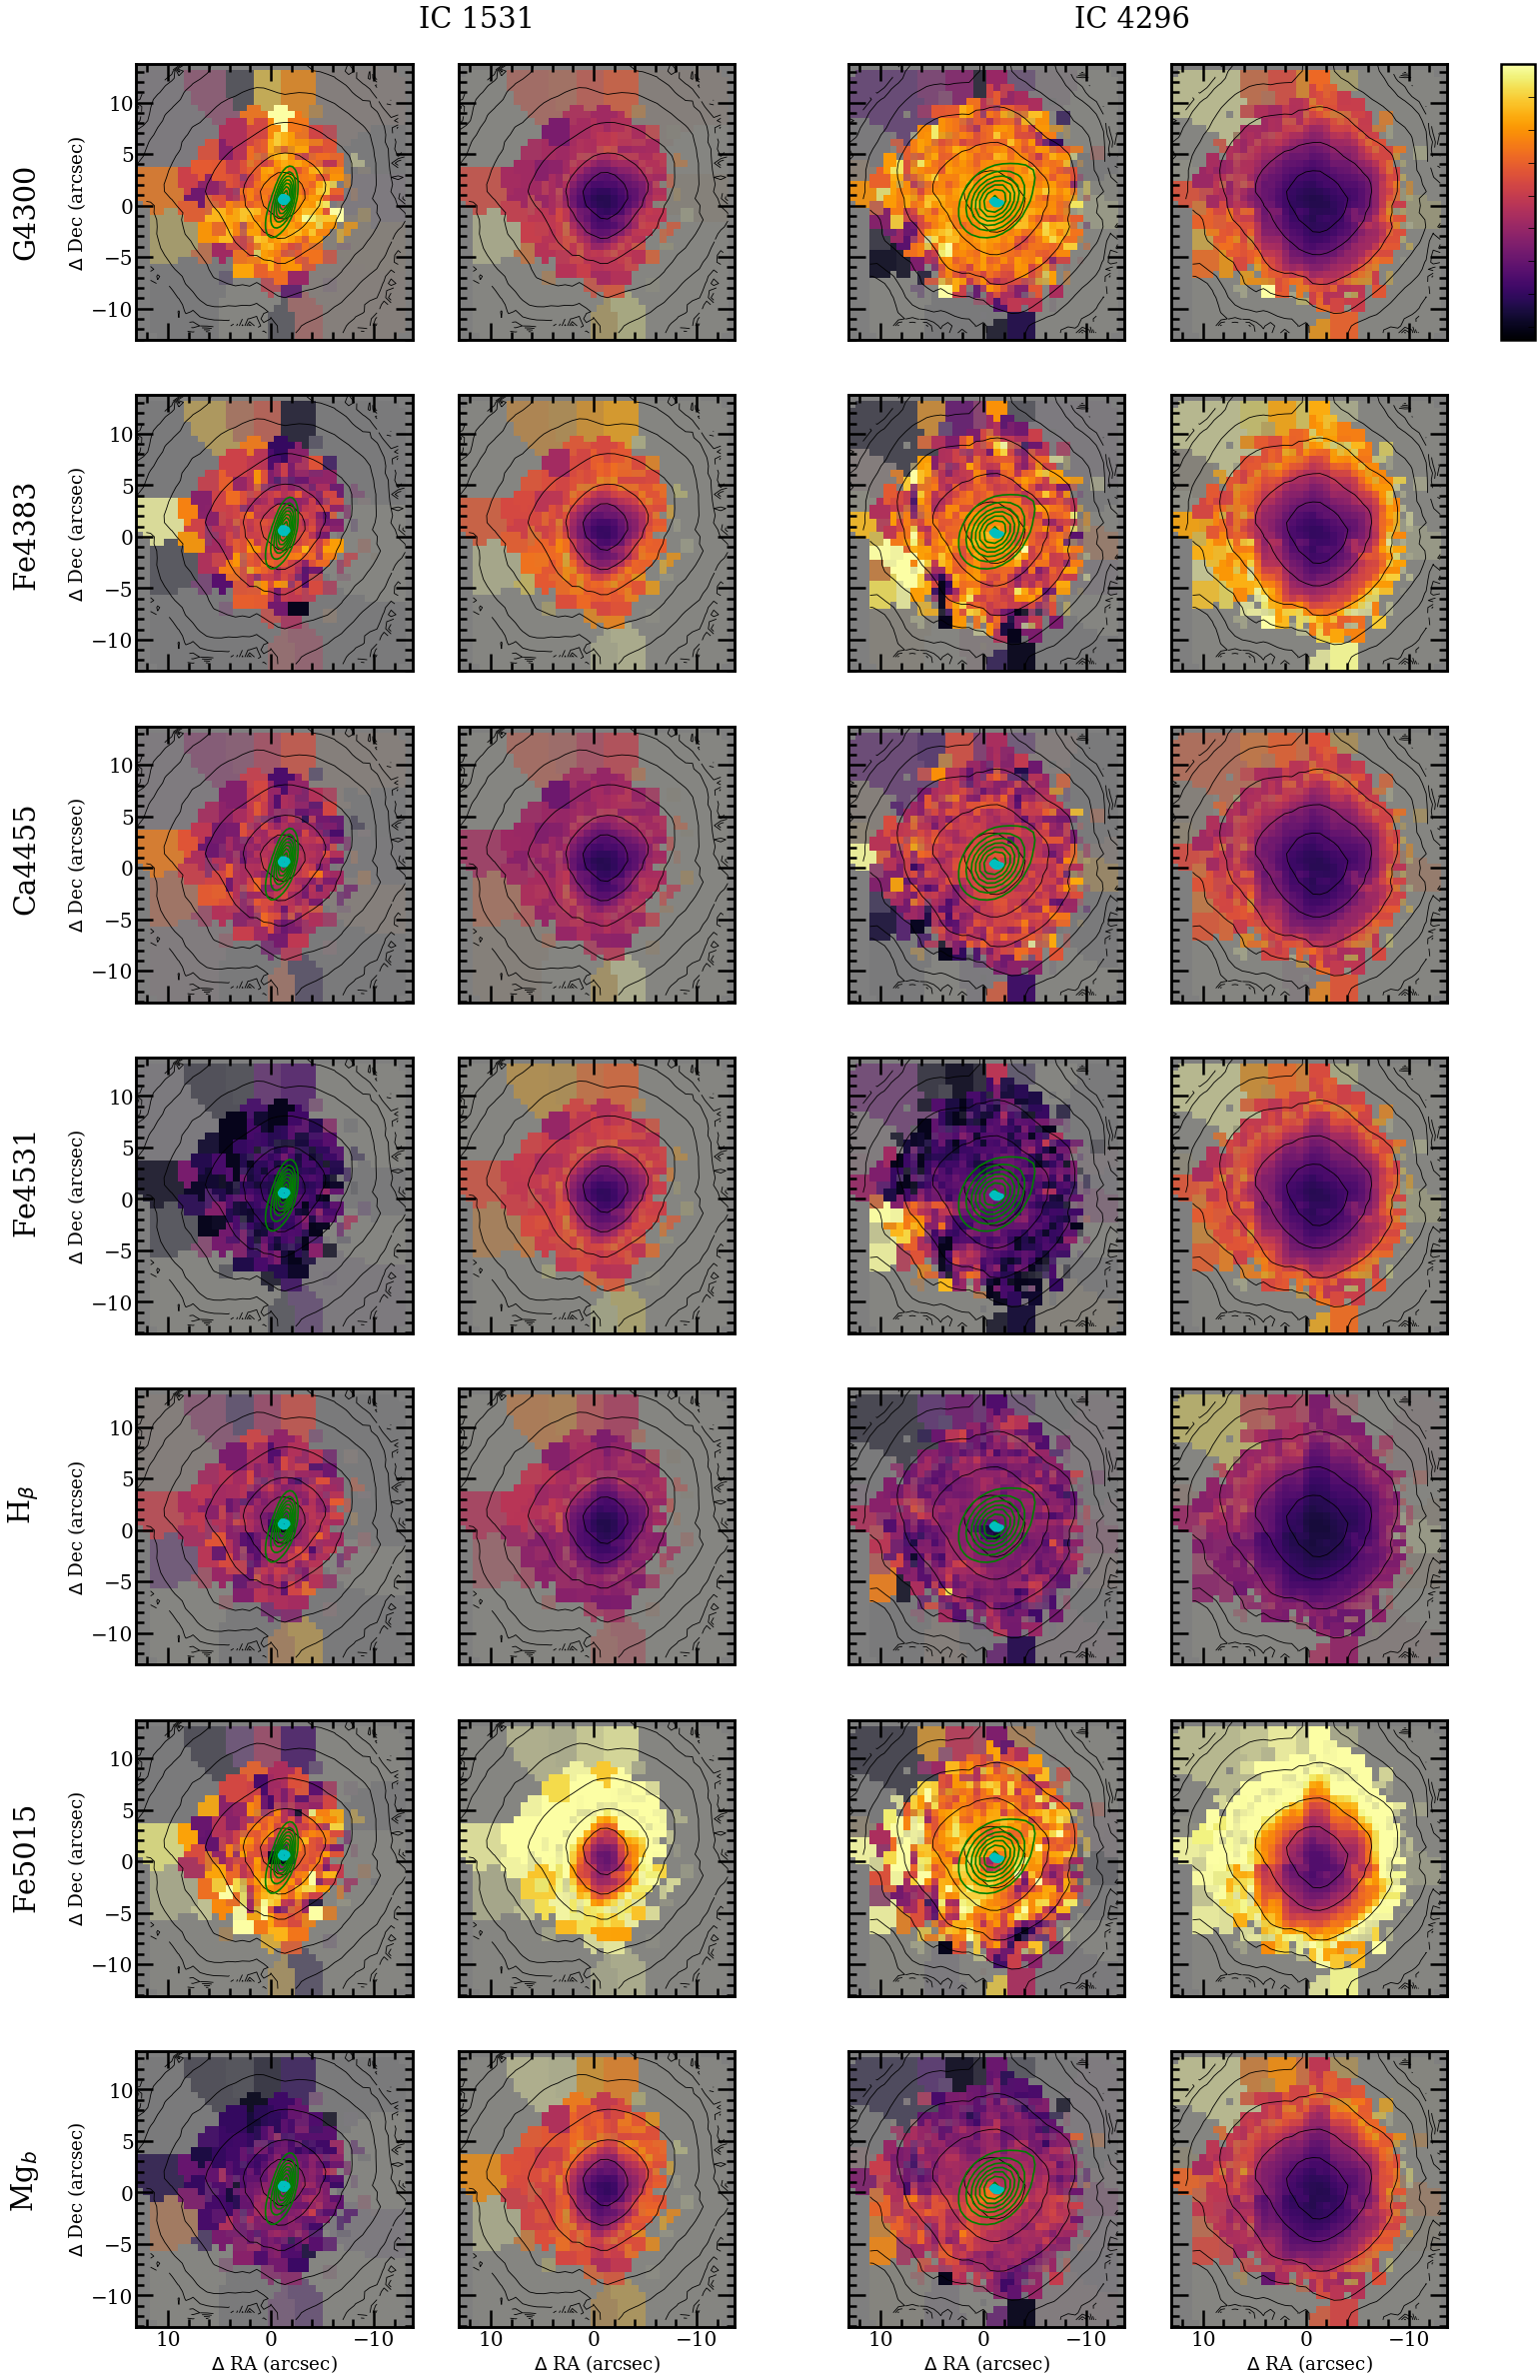
\includegraphics[height=0.94\textheight]{chapter4/vimos/abs2.png}
			\contcaption{continued for IC 1531 and IC 4296.}
		\end{figure*}
		\begin{figure*}
			\centering
			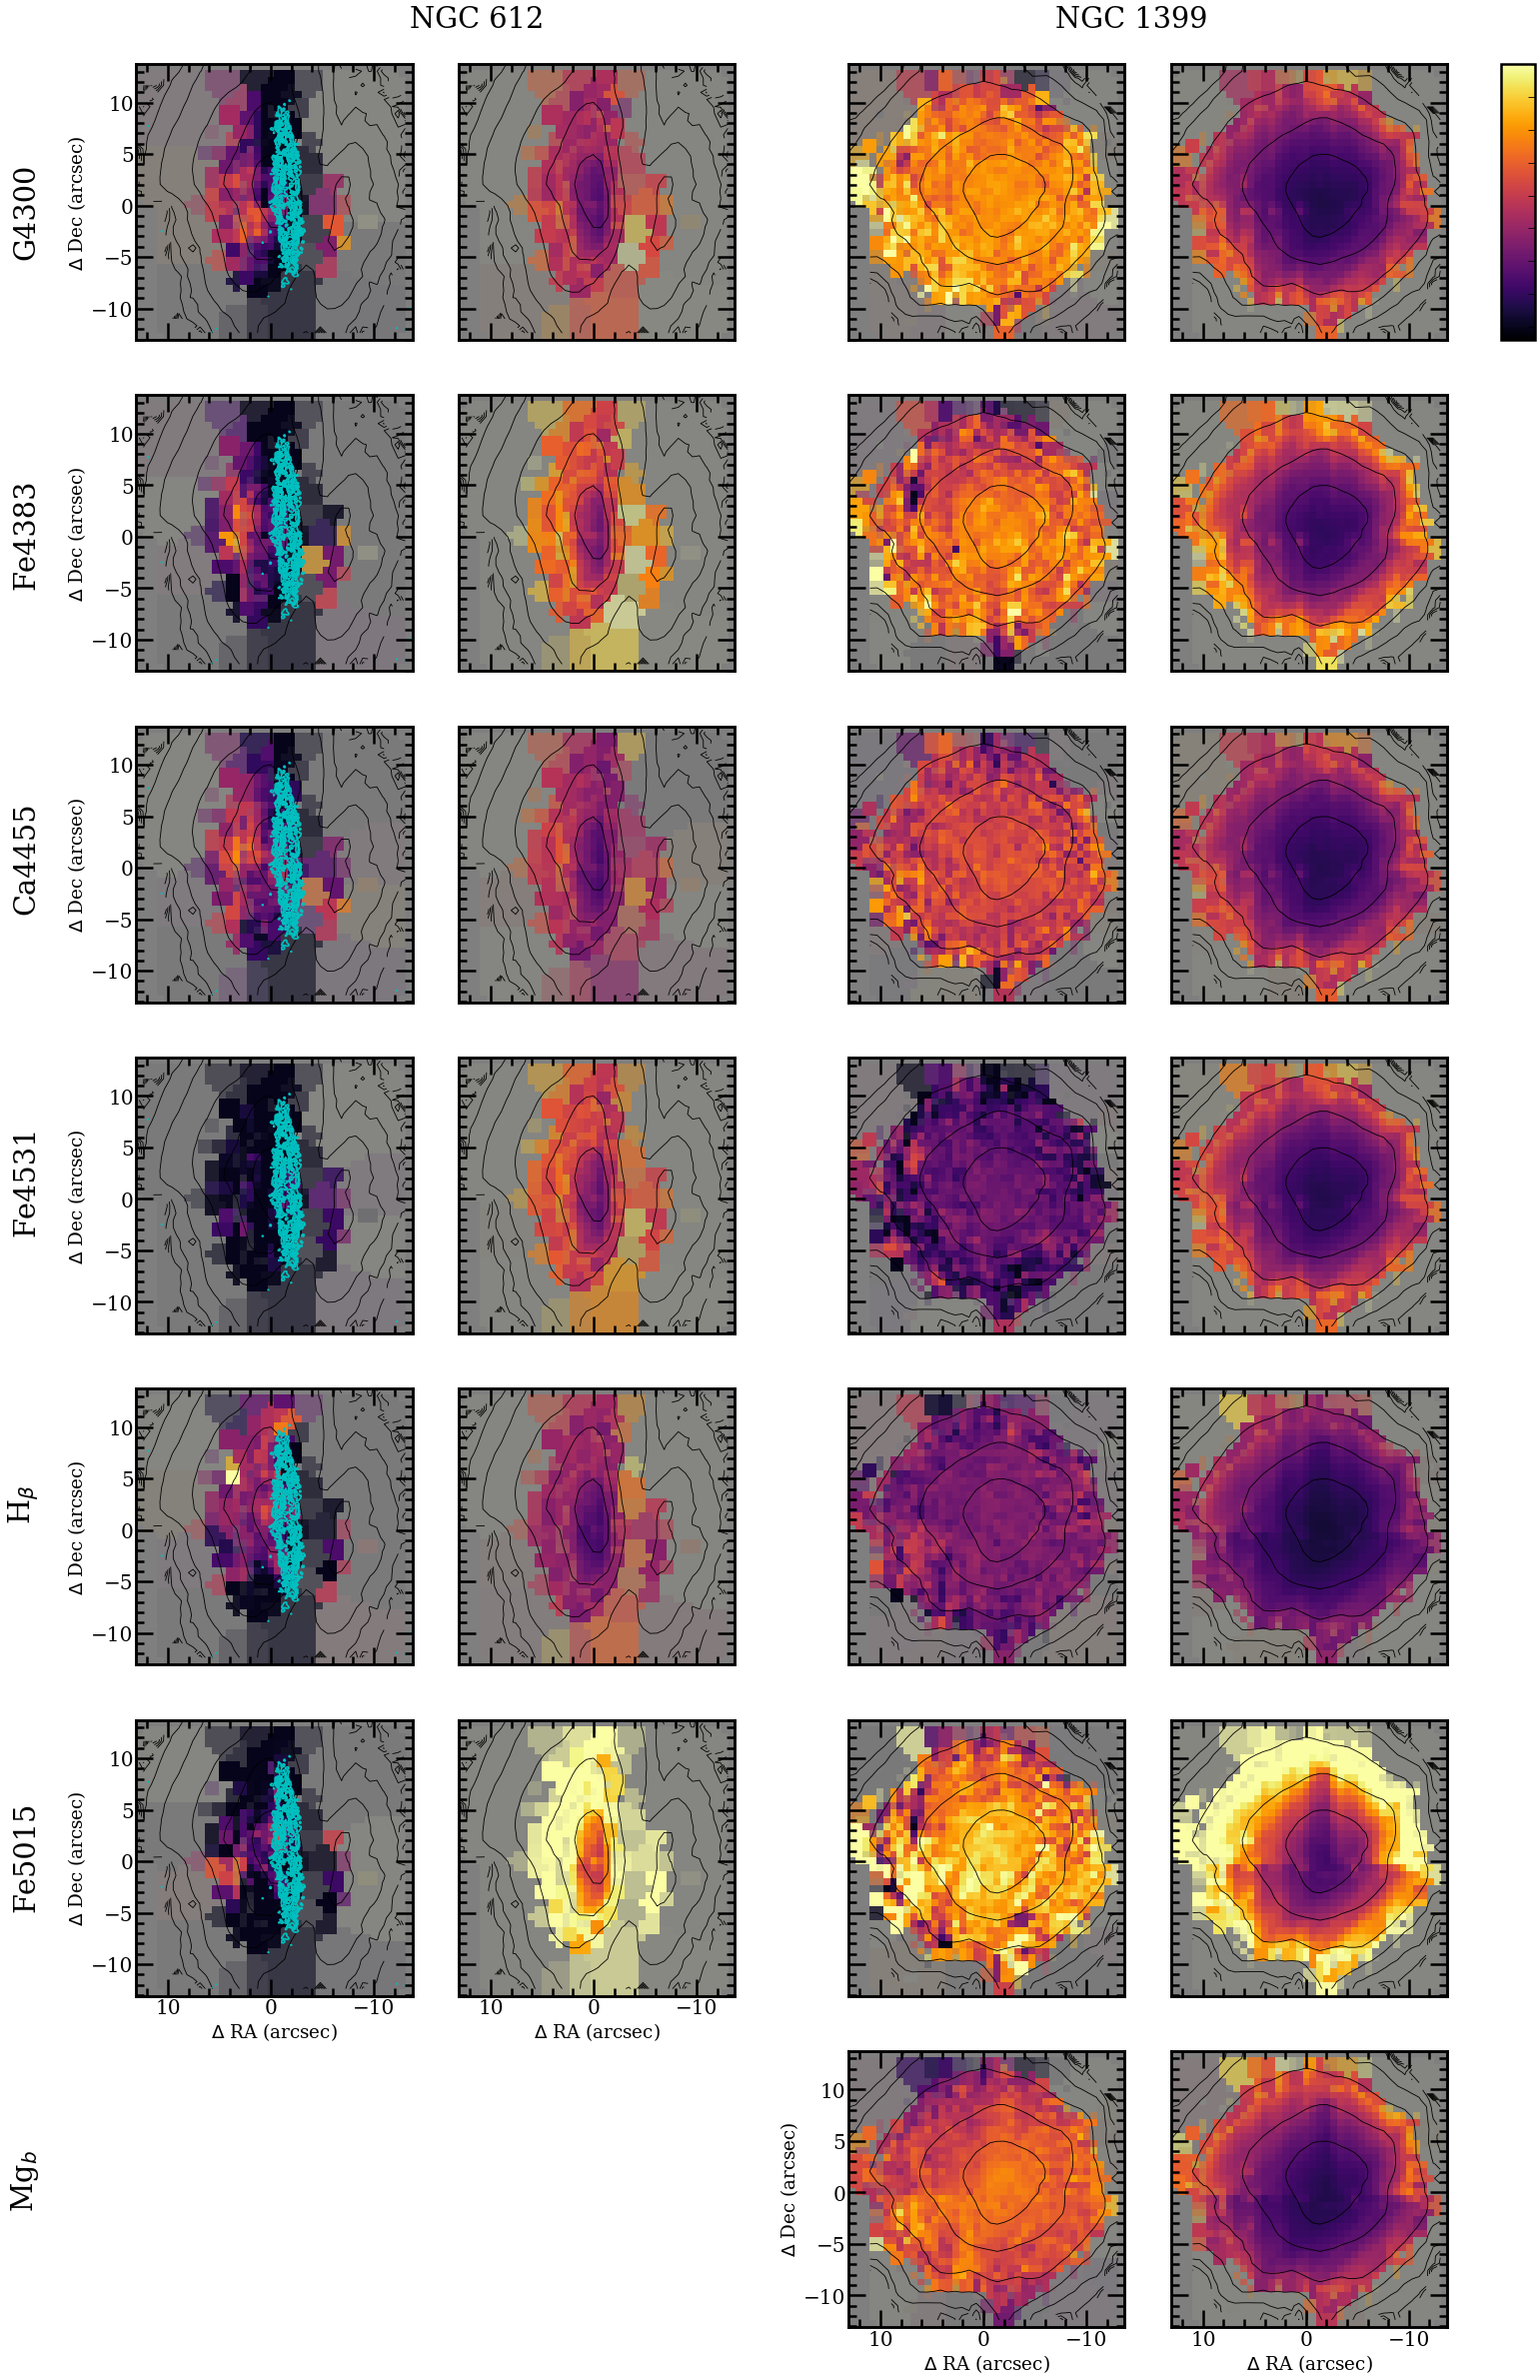
\includegraphics[height=0.94\textheight]{chapter4/vimos/abs3.png}
			\contcaption{continued for NGC 612 and NGC 1399}
		\end{figure*}
		\begin{figure*}
			\centering
			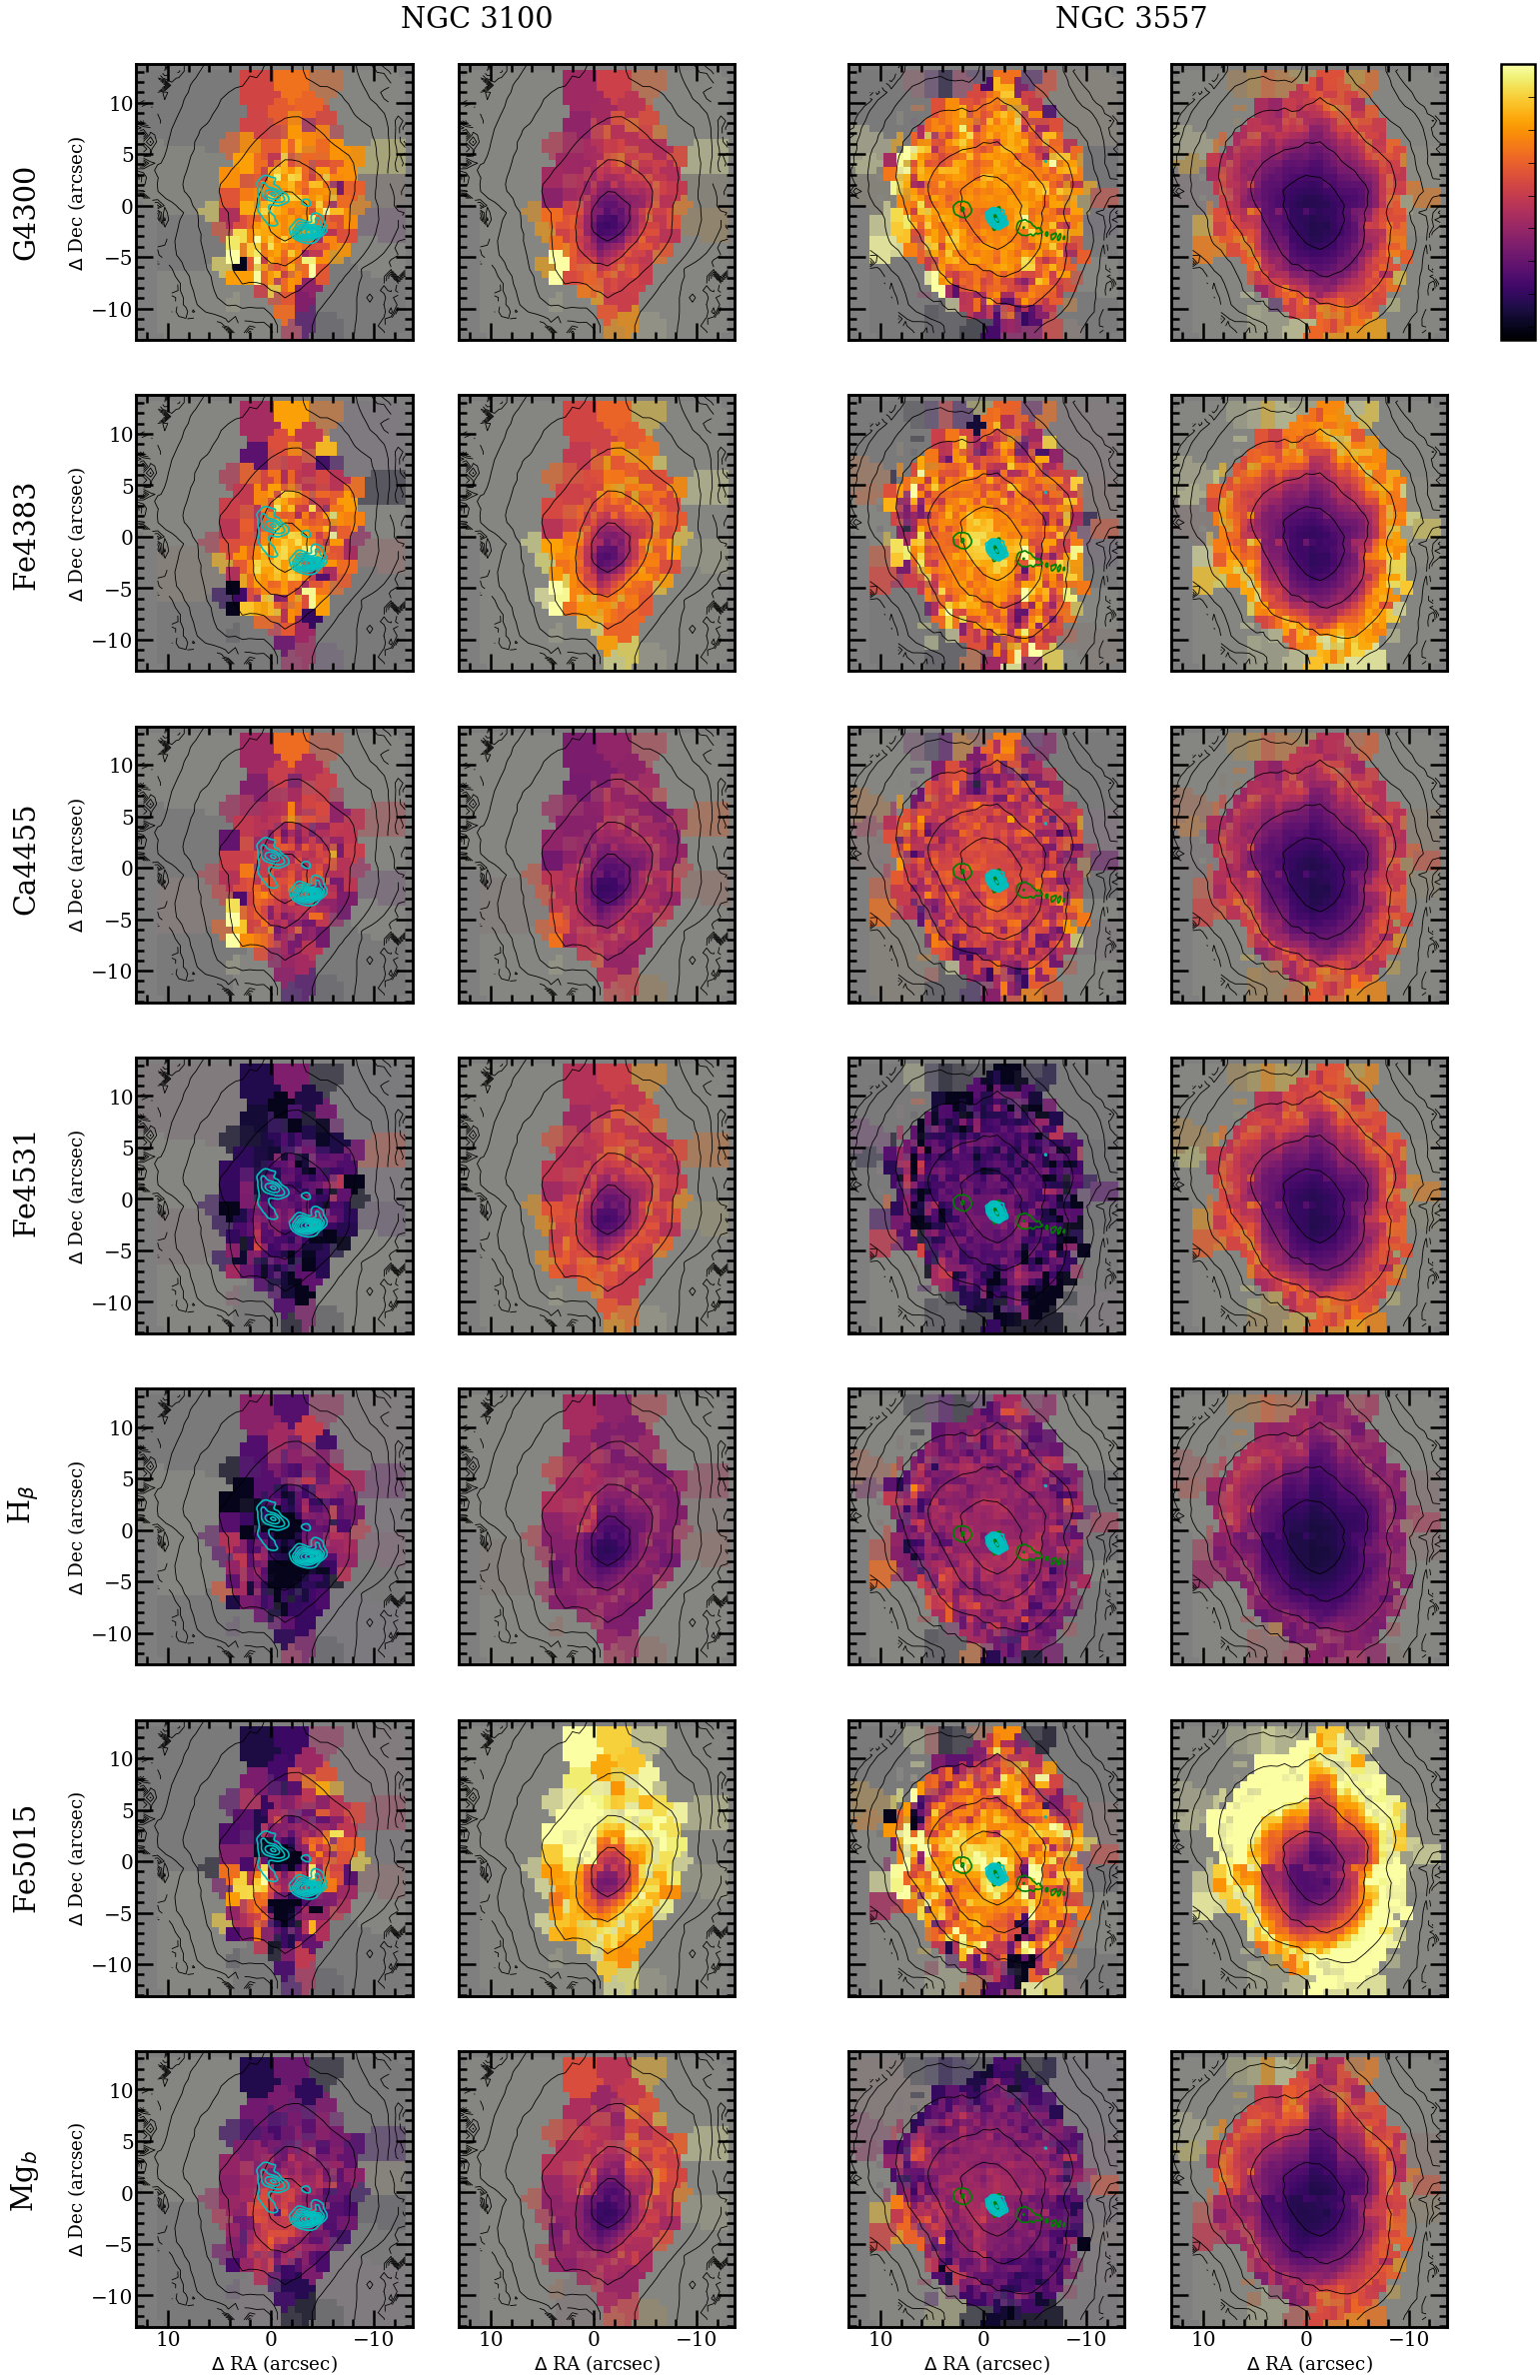
\includegraphics[height=0.94\textheight]{chapter4/vimos/abs4.png}
			\contcaption{continued for NGC 3100 and NGC 3557}
		\end{figure*}
		\begin{figure*}
			\centering
			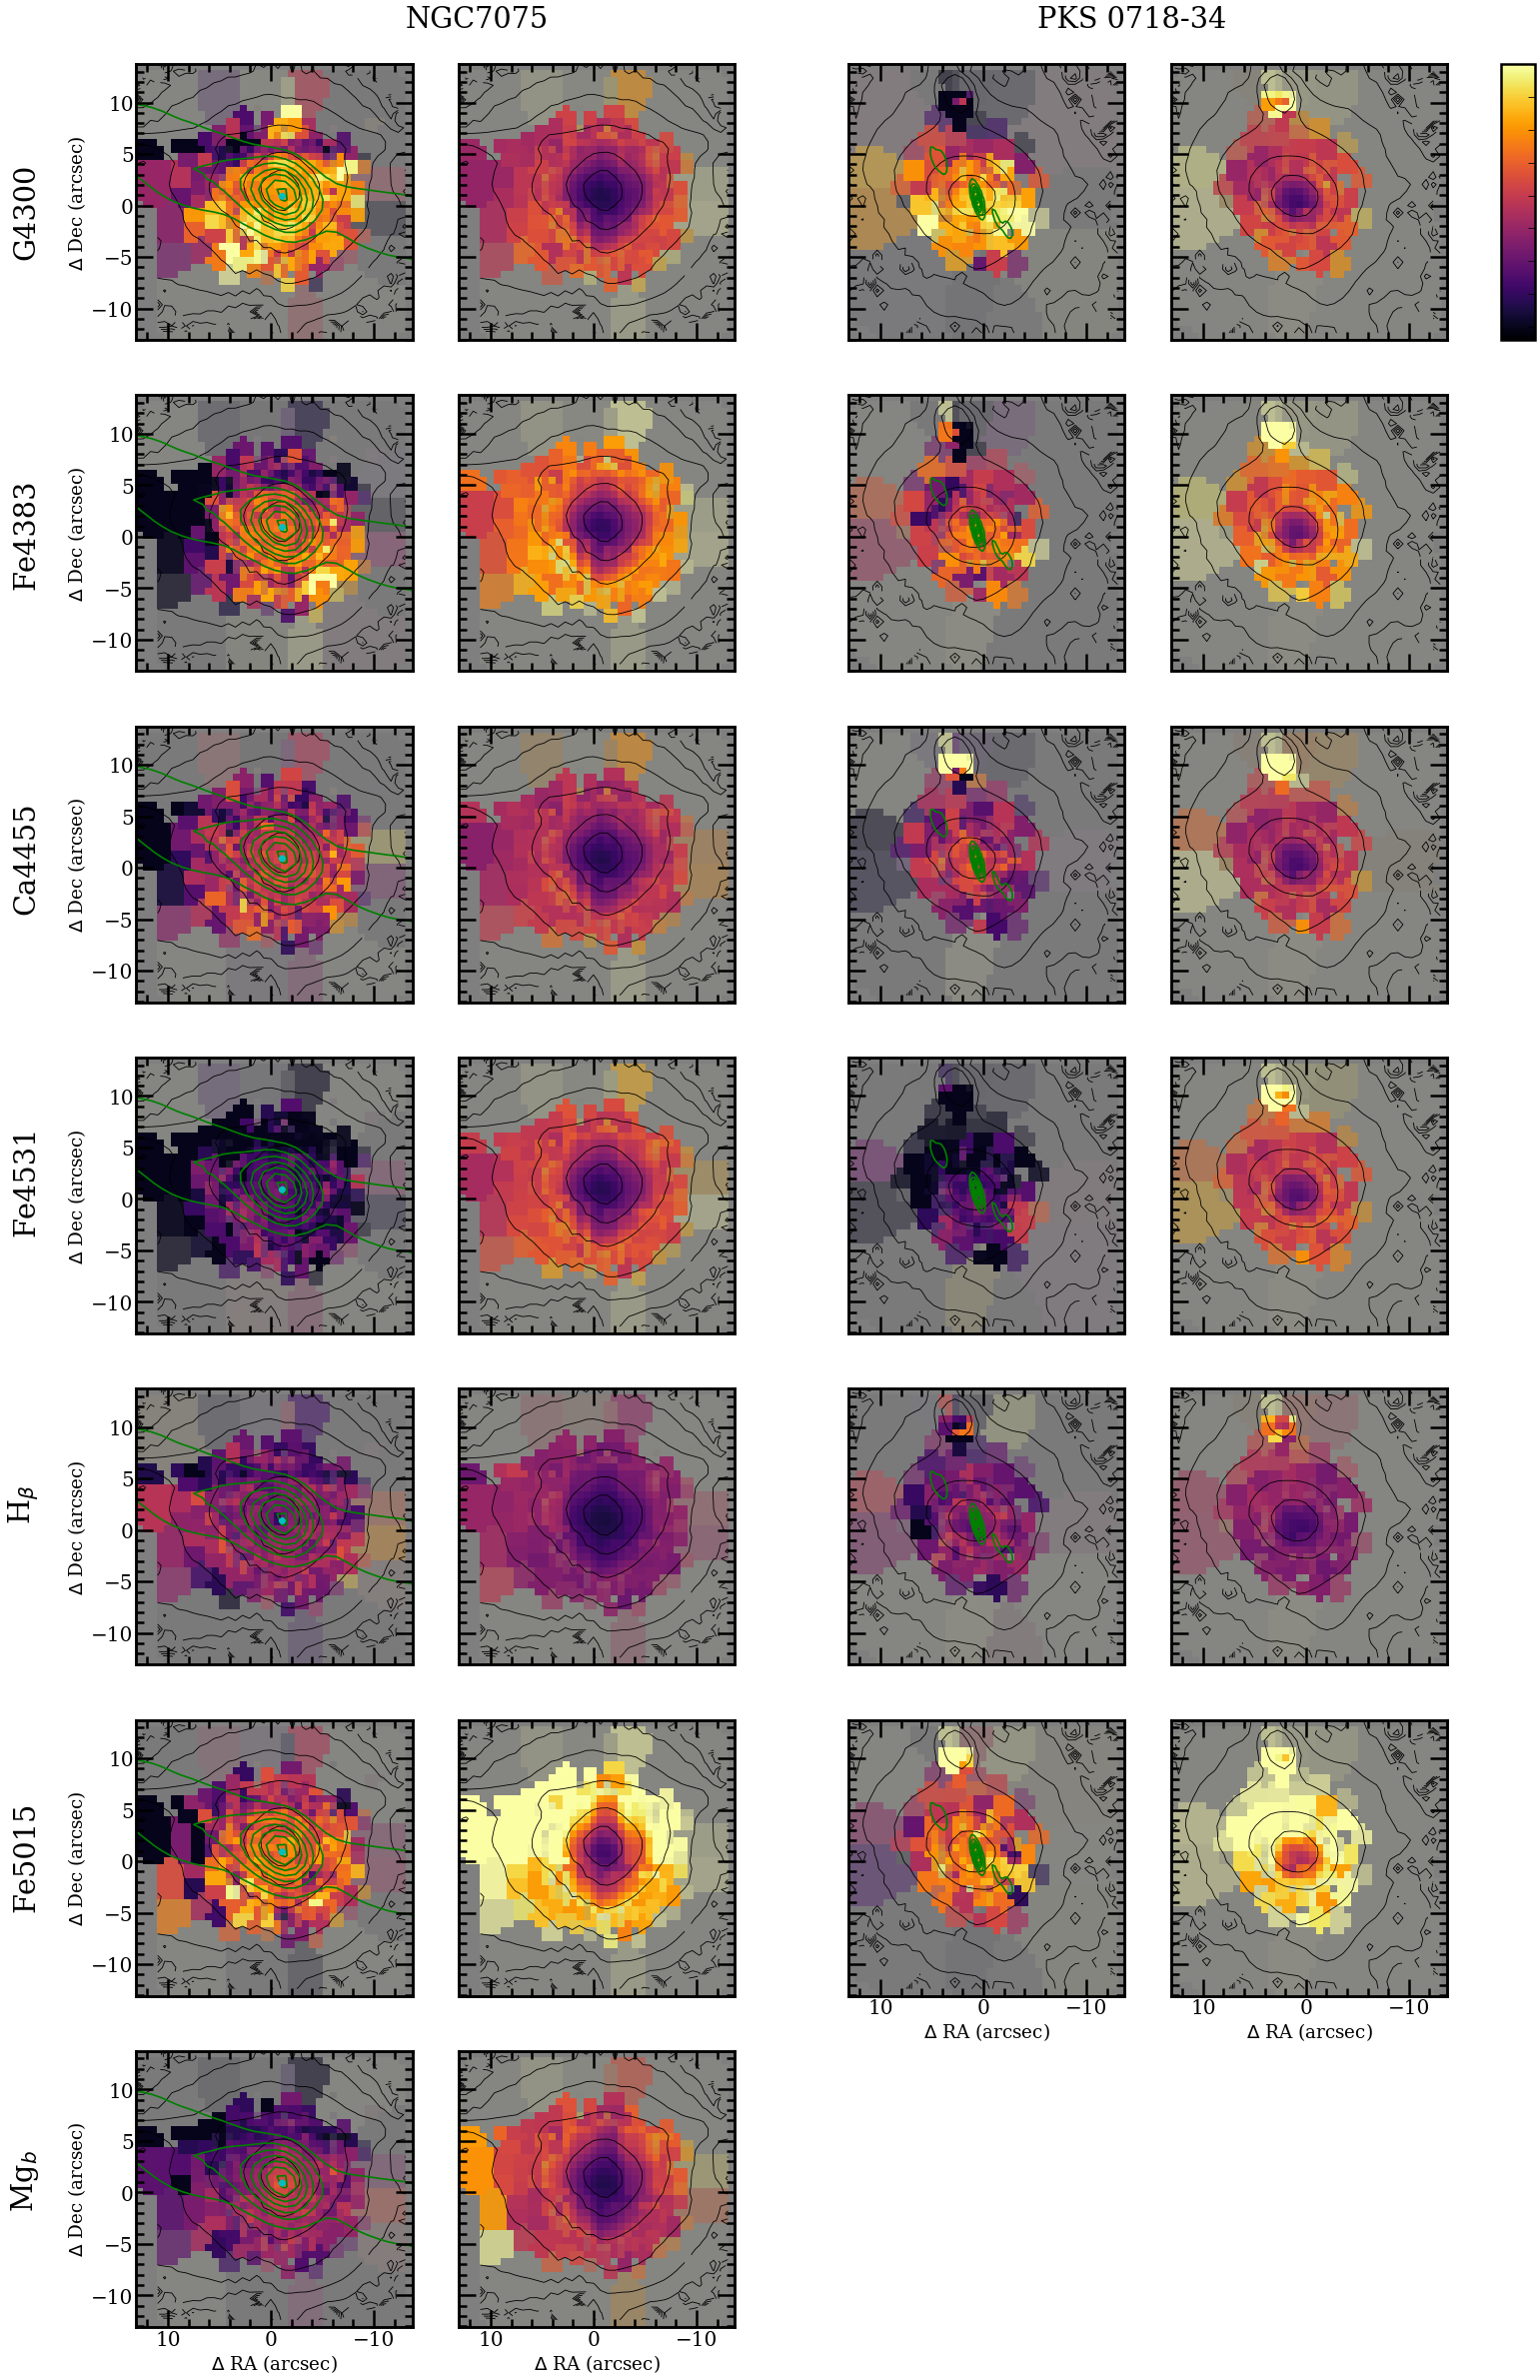
\includegraphics[height=0.94\textheight]{chapter4/vimos/abs5.png}
			\contcaption{continued for NGC 7075 and PKS 718-34}
		\end{figure*}

		\begin{figure*}
			\centering
			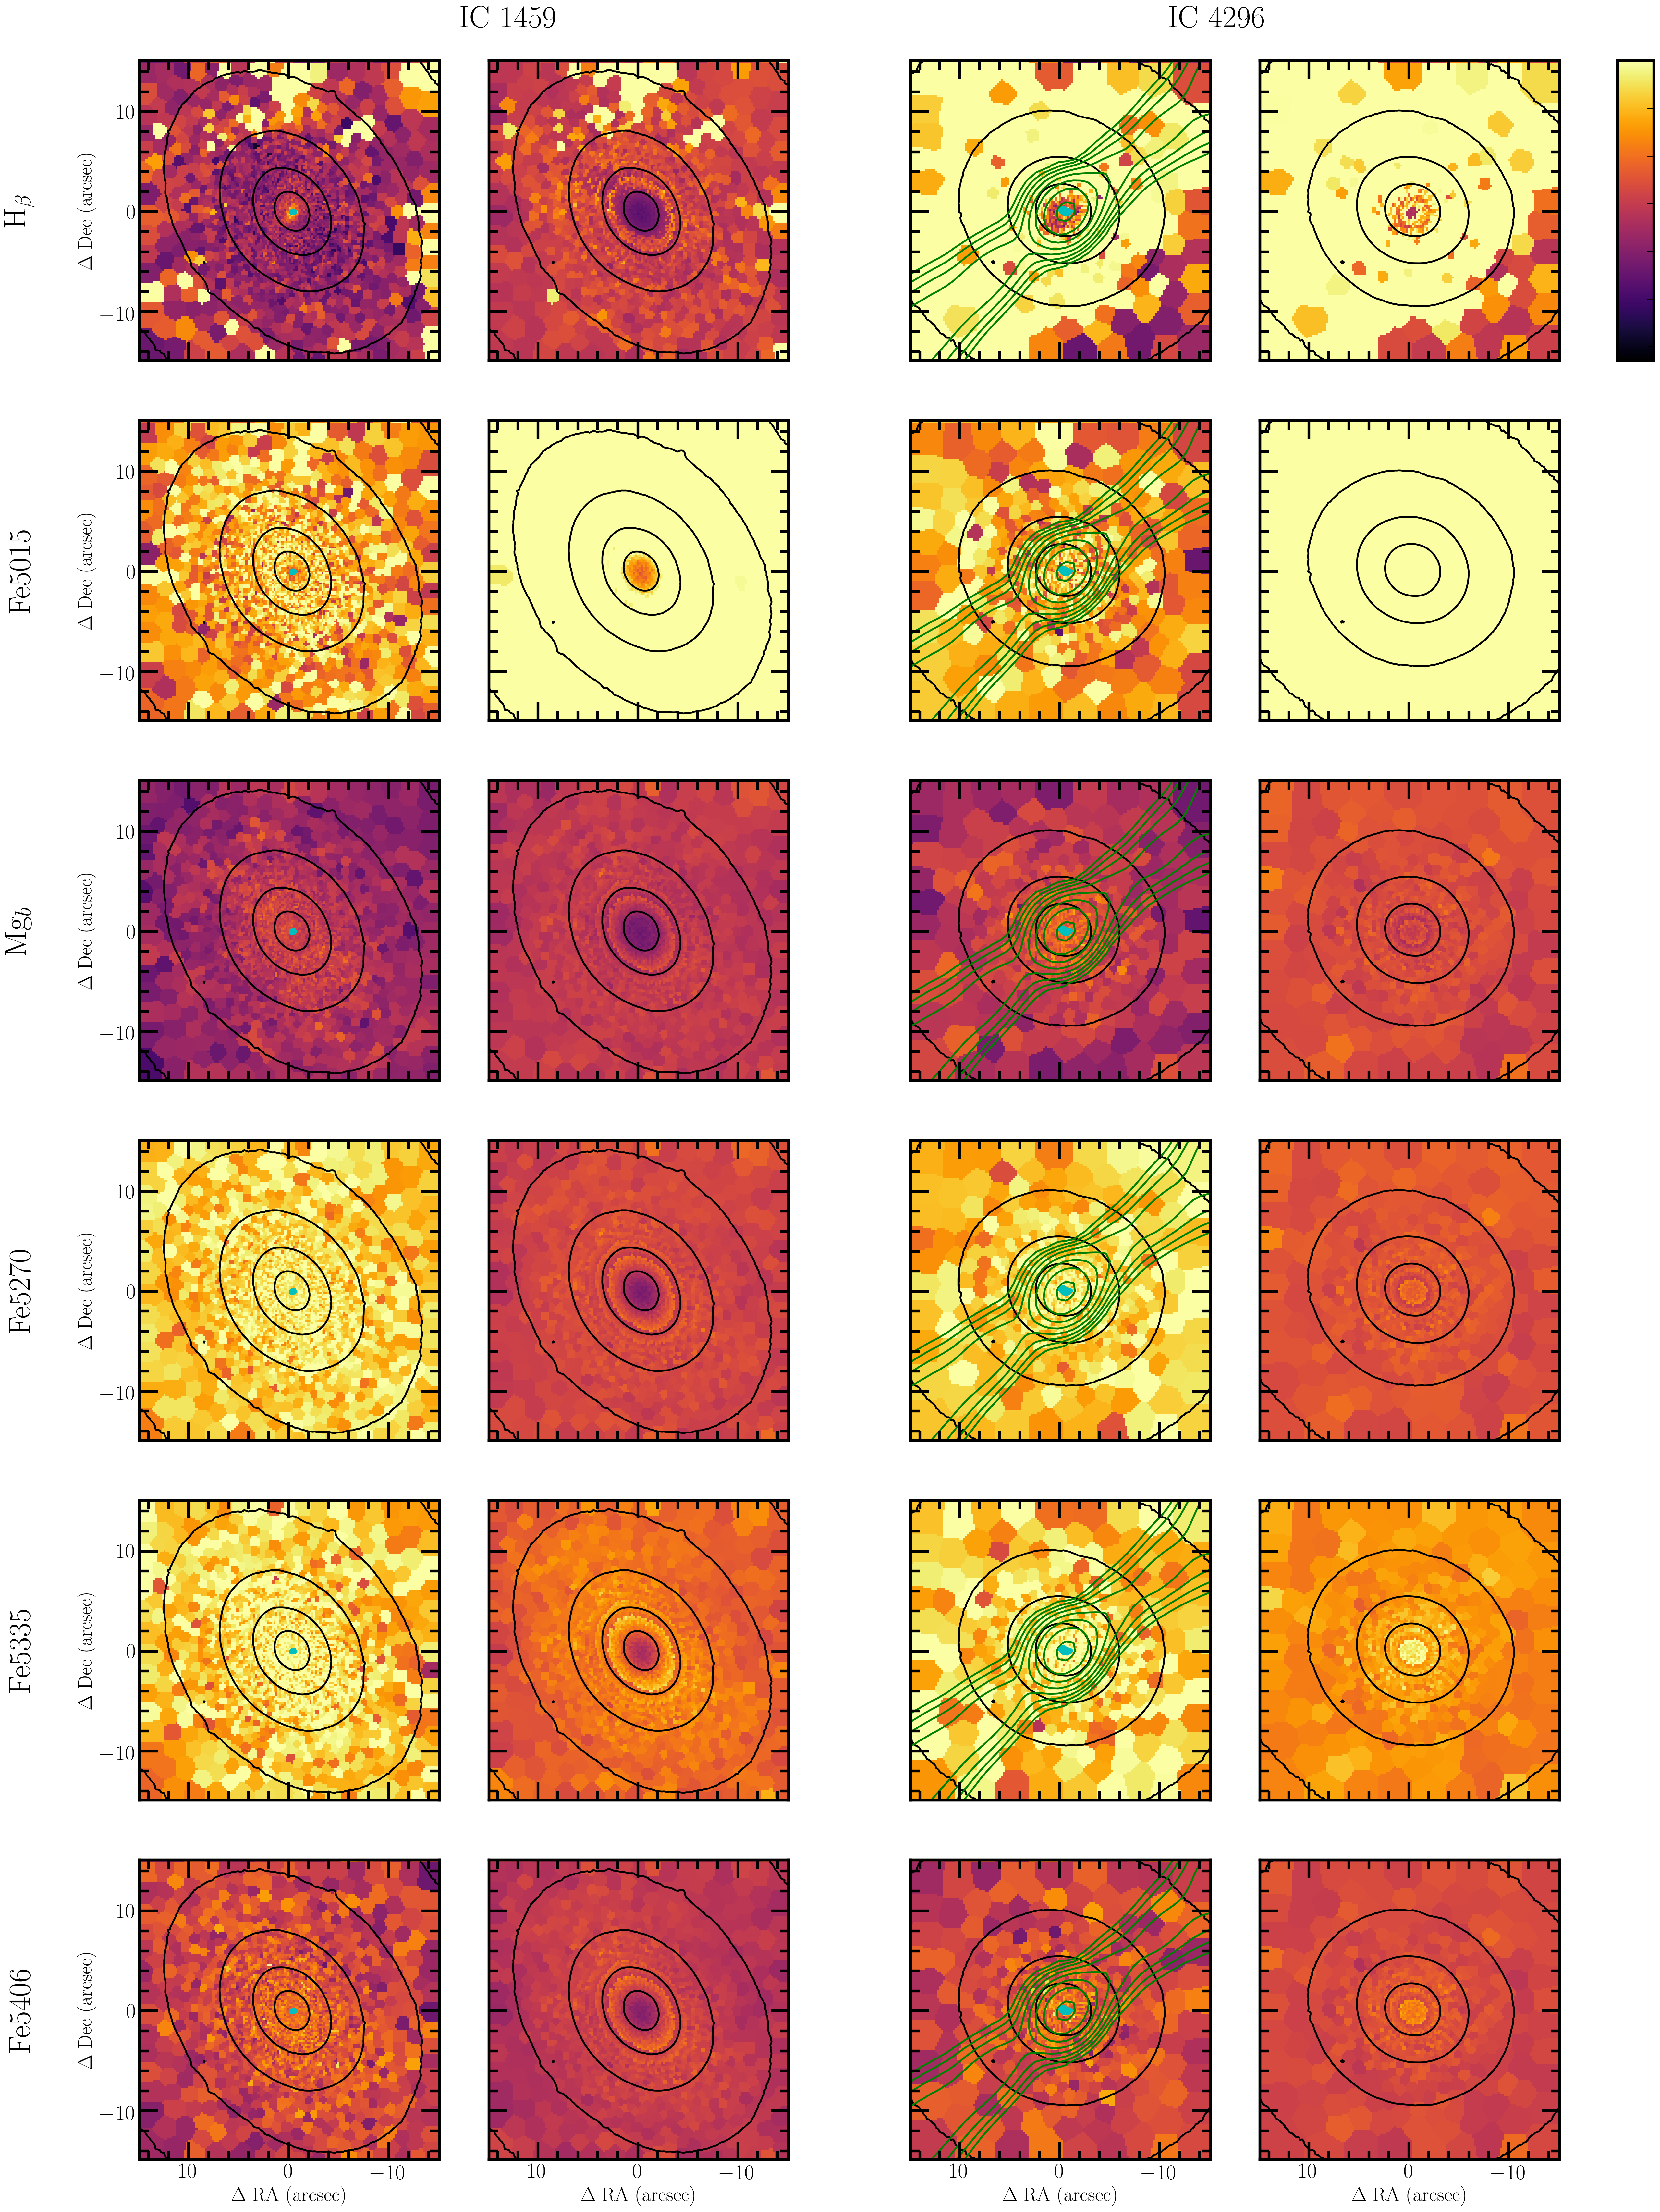
\includegraphics[height=0.94\textheight]{chapter4/muse/abs1.png}
			\caption[MUSE absorption line strength maps]{MUSE stellar kinematic maps: From left to right: IC1459, IC1459 uncertainties, IC4296 and IC4296 uncertainties. From top to bottom: H$_\beta$, Fe5015, Mg$_b$, Fe5270, Fe5335, Fe5406, Fe5709. Plots are as in \ref{fig:VIMOS_stellar}}
			\label{fig:MUSE_absorption}
		\end{figure*}
		\begin{figure*}
			\centering
			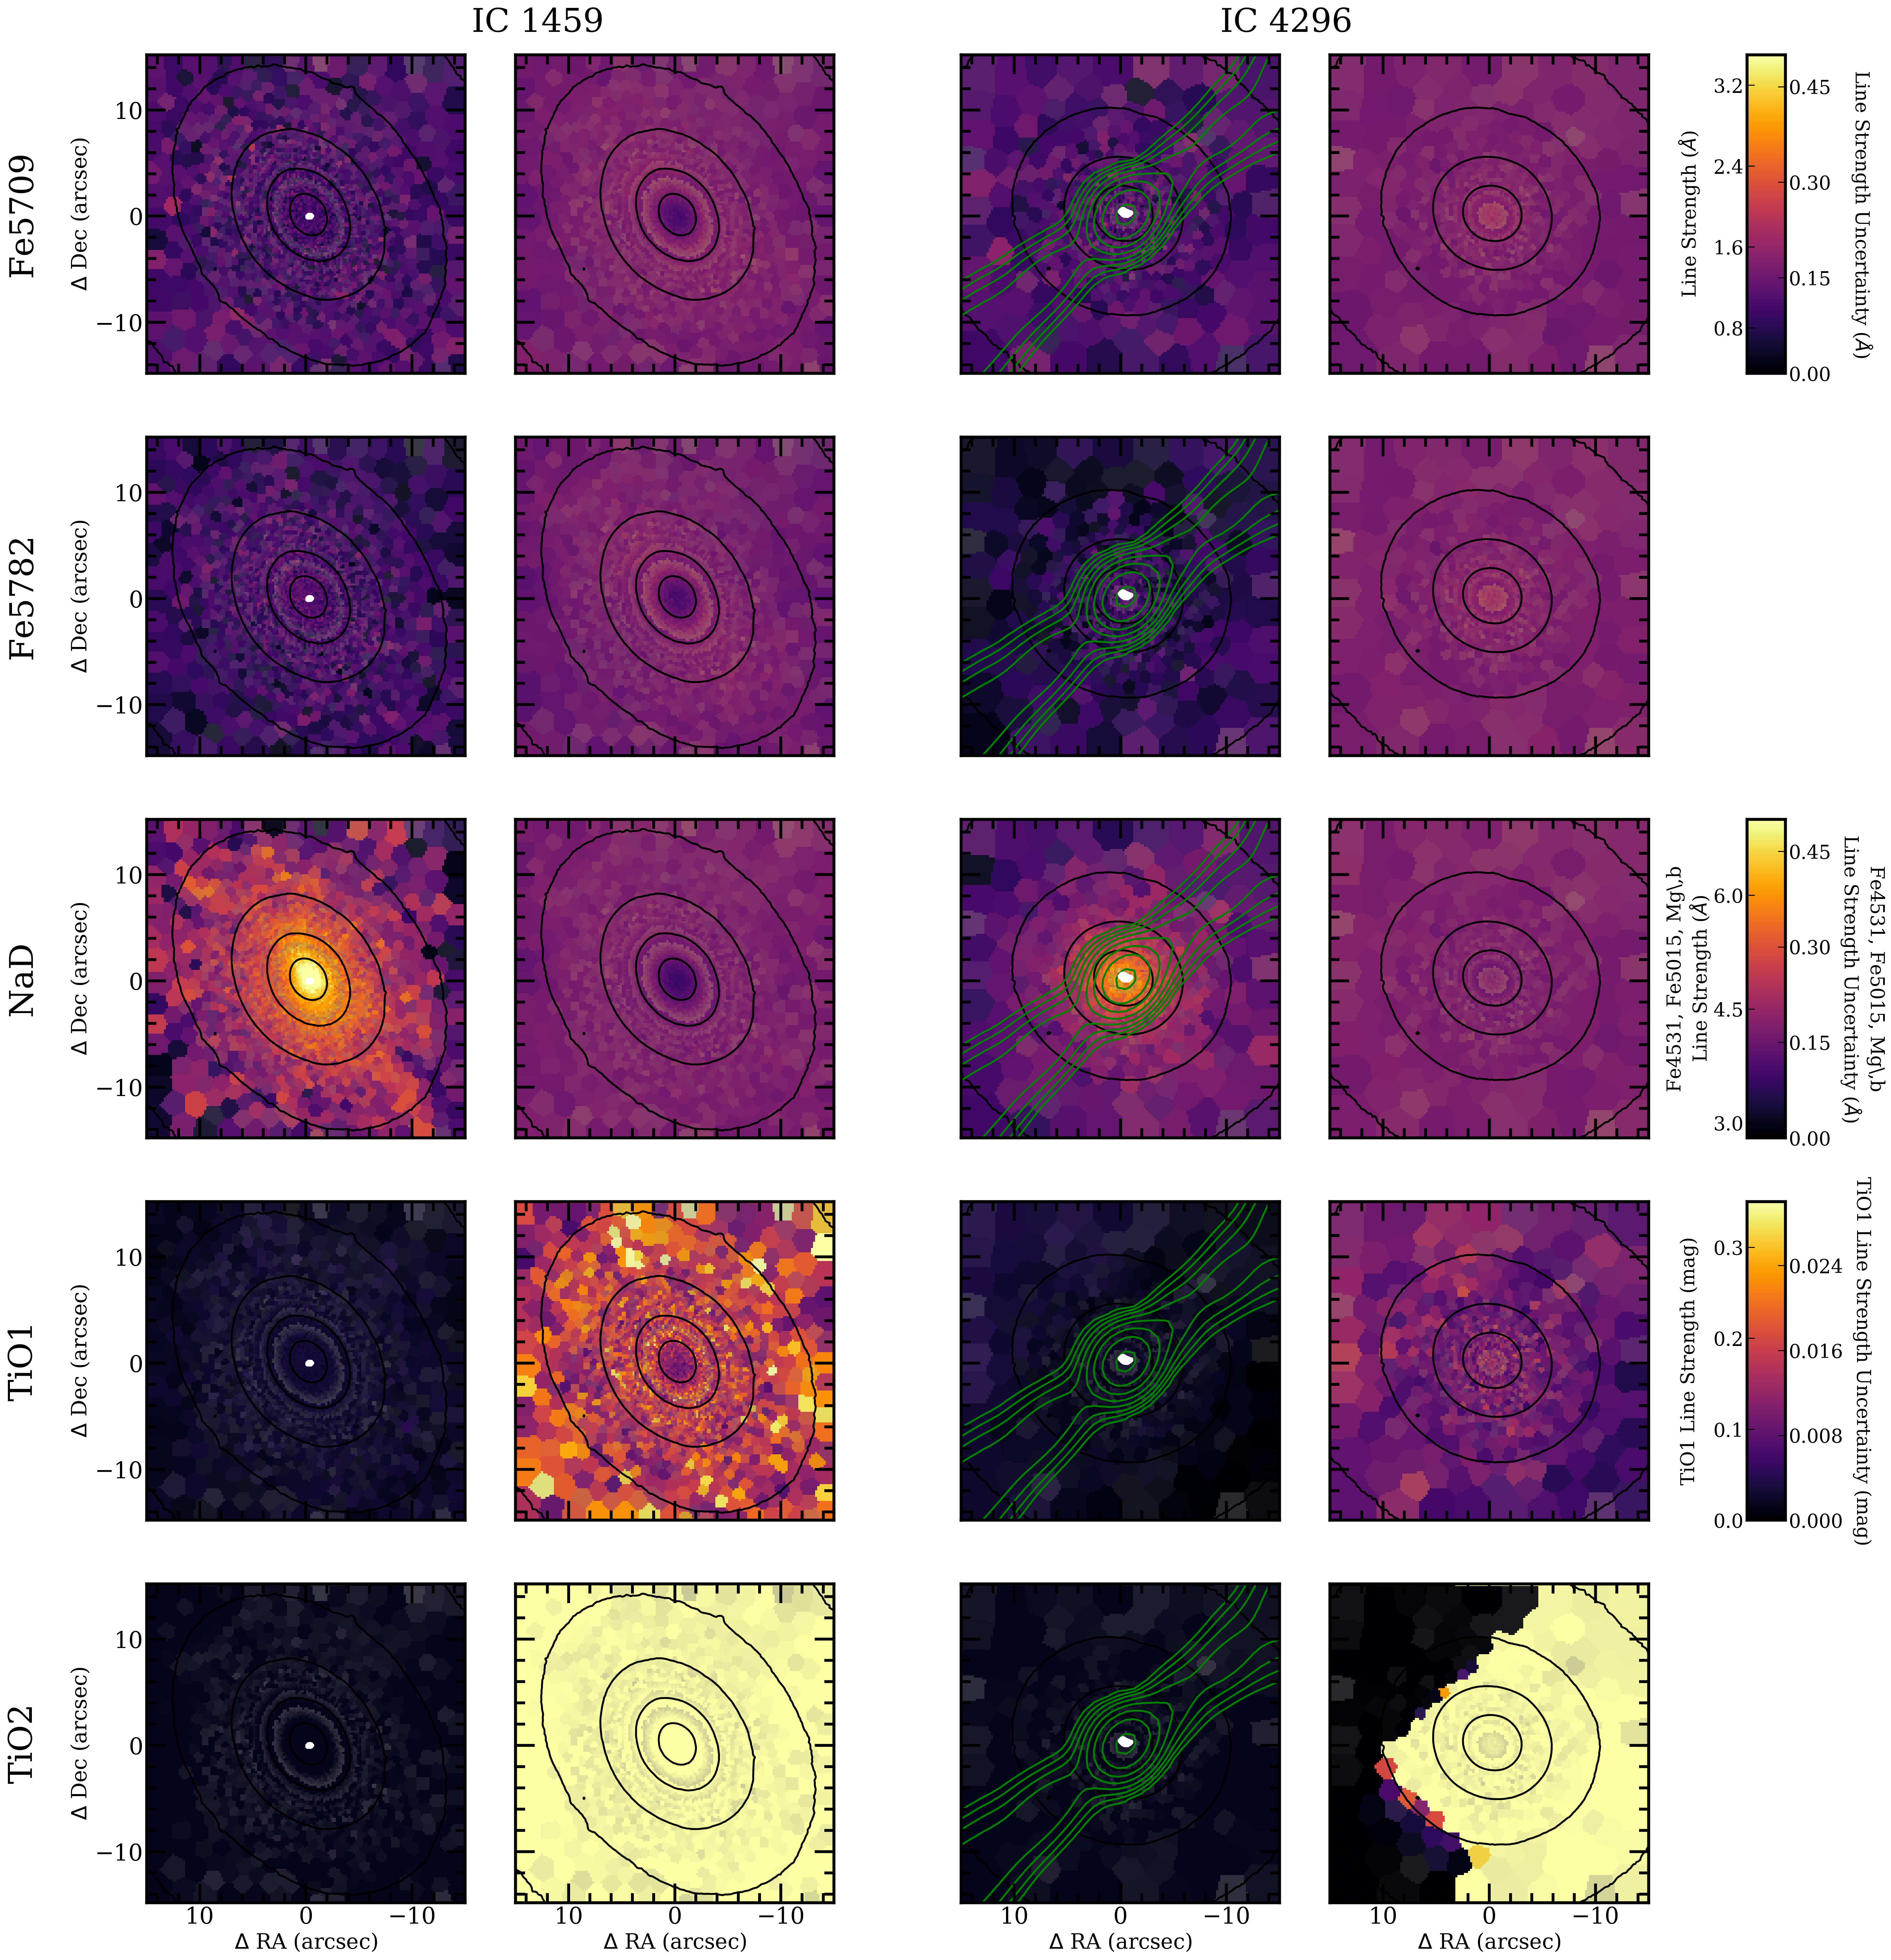
\includegraphics[height=0.54\textheight]{chapter4/muse/abs1b.png}
			\contcaption{continued: From top to bottom: Fe5782, NaD, TiO1, TiO2. Plots are as in \ref{fig:VIMOS_stellar}}
		\end{figure*}
		\begin{figure*}
			\centering
			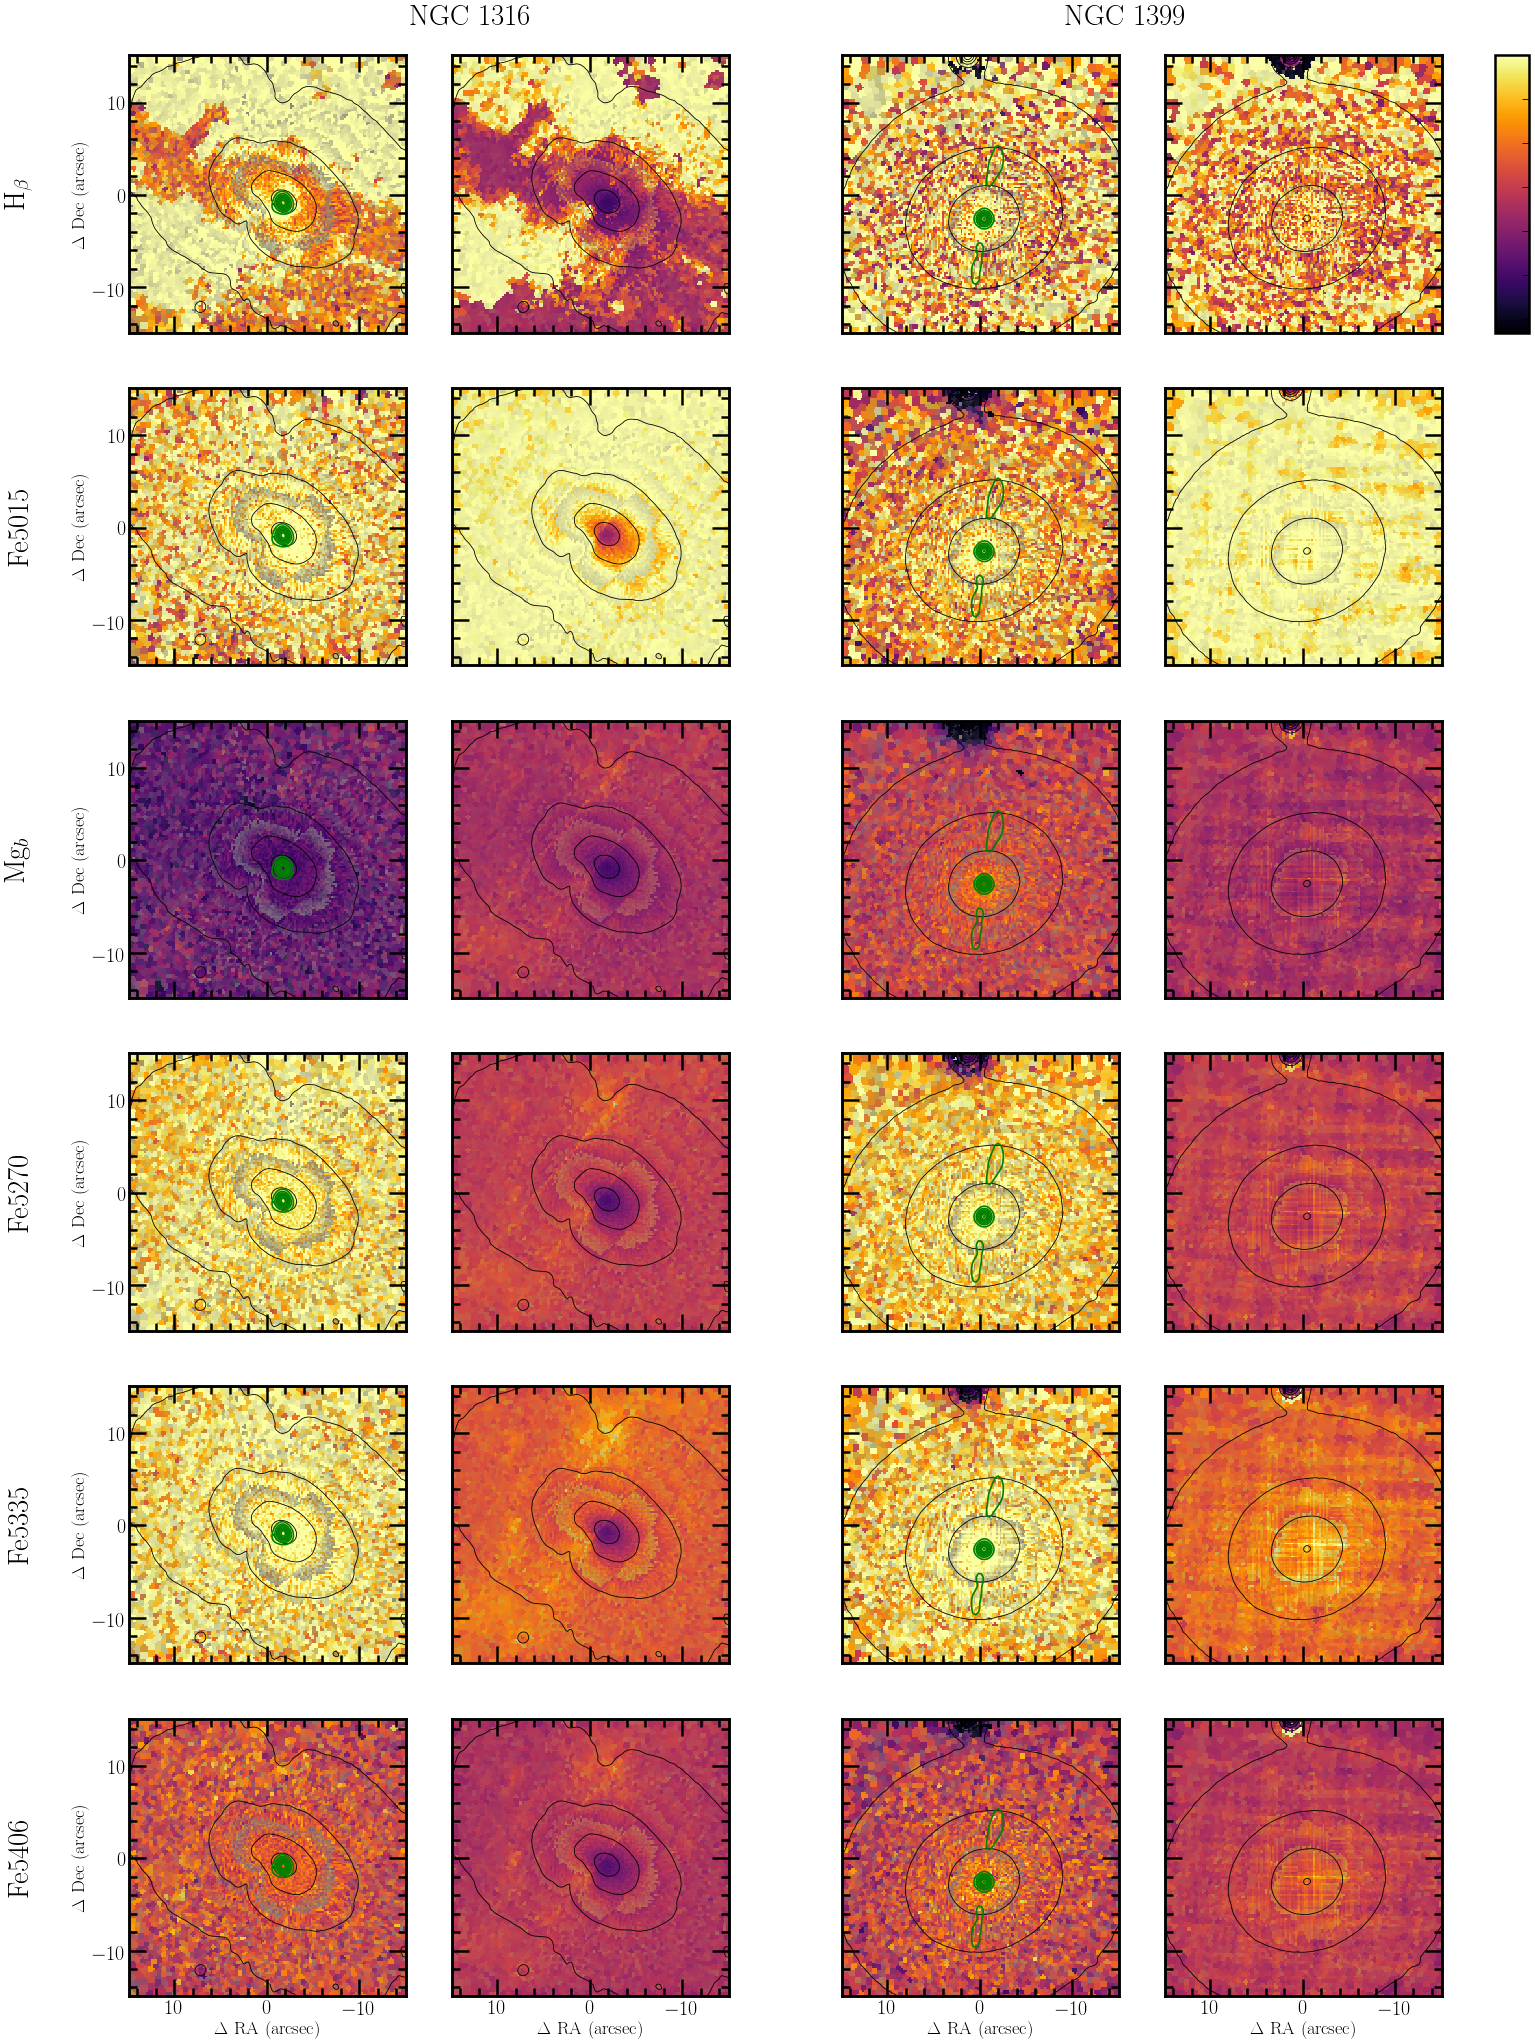
\includegraphics[height=0.94\textheight]{chapter4/muse/abs2.png}
			\contcaption{continued for NGC1316 and NGC1399.}
		\end{figure*}
		\begin{figure*}
			\centering
			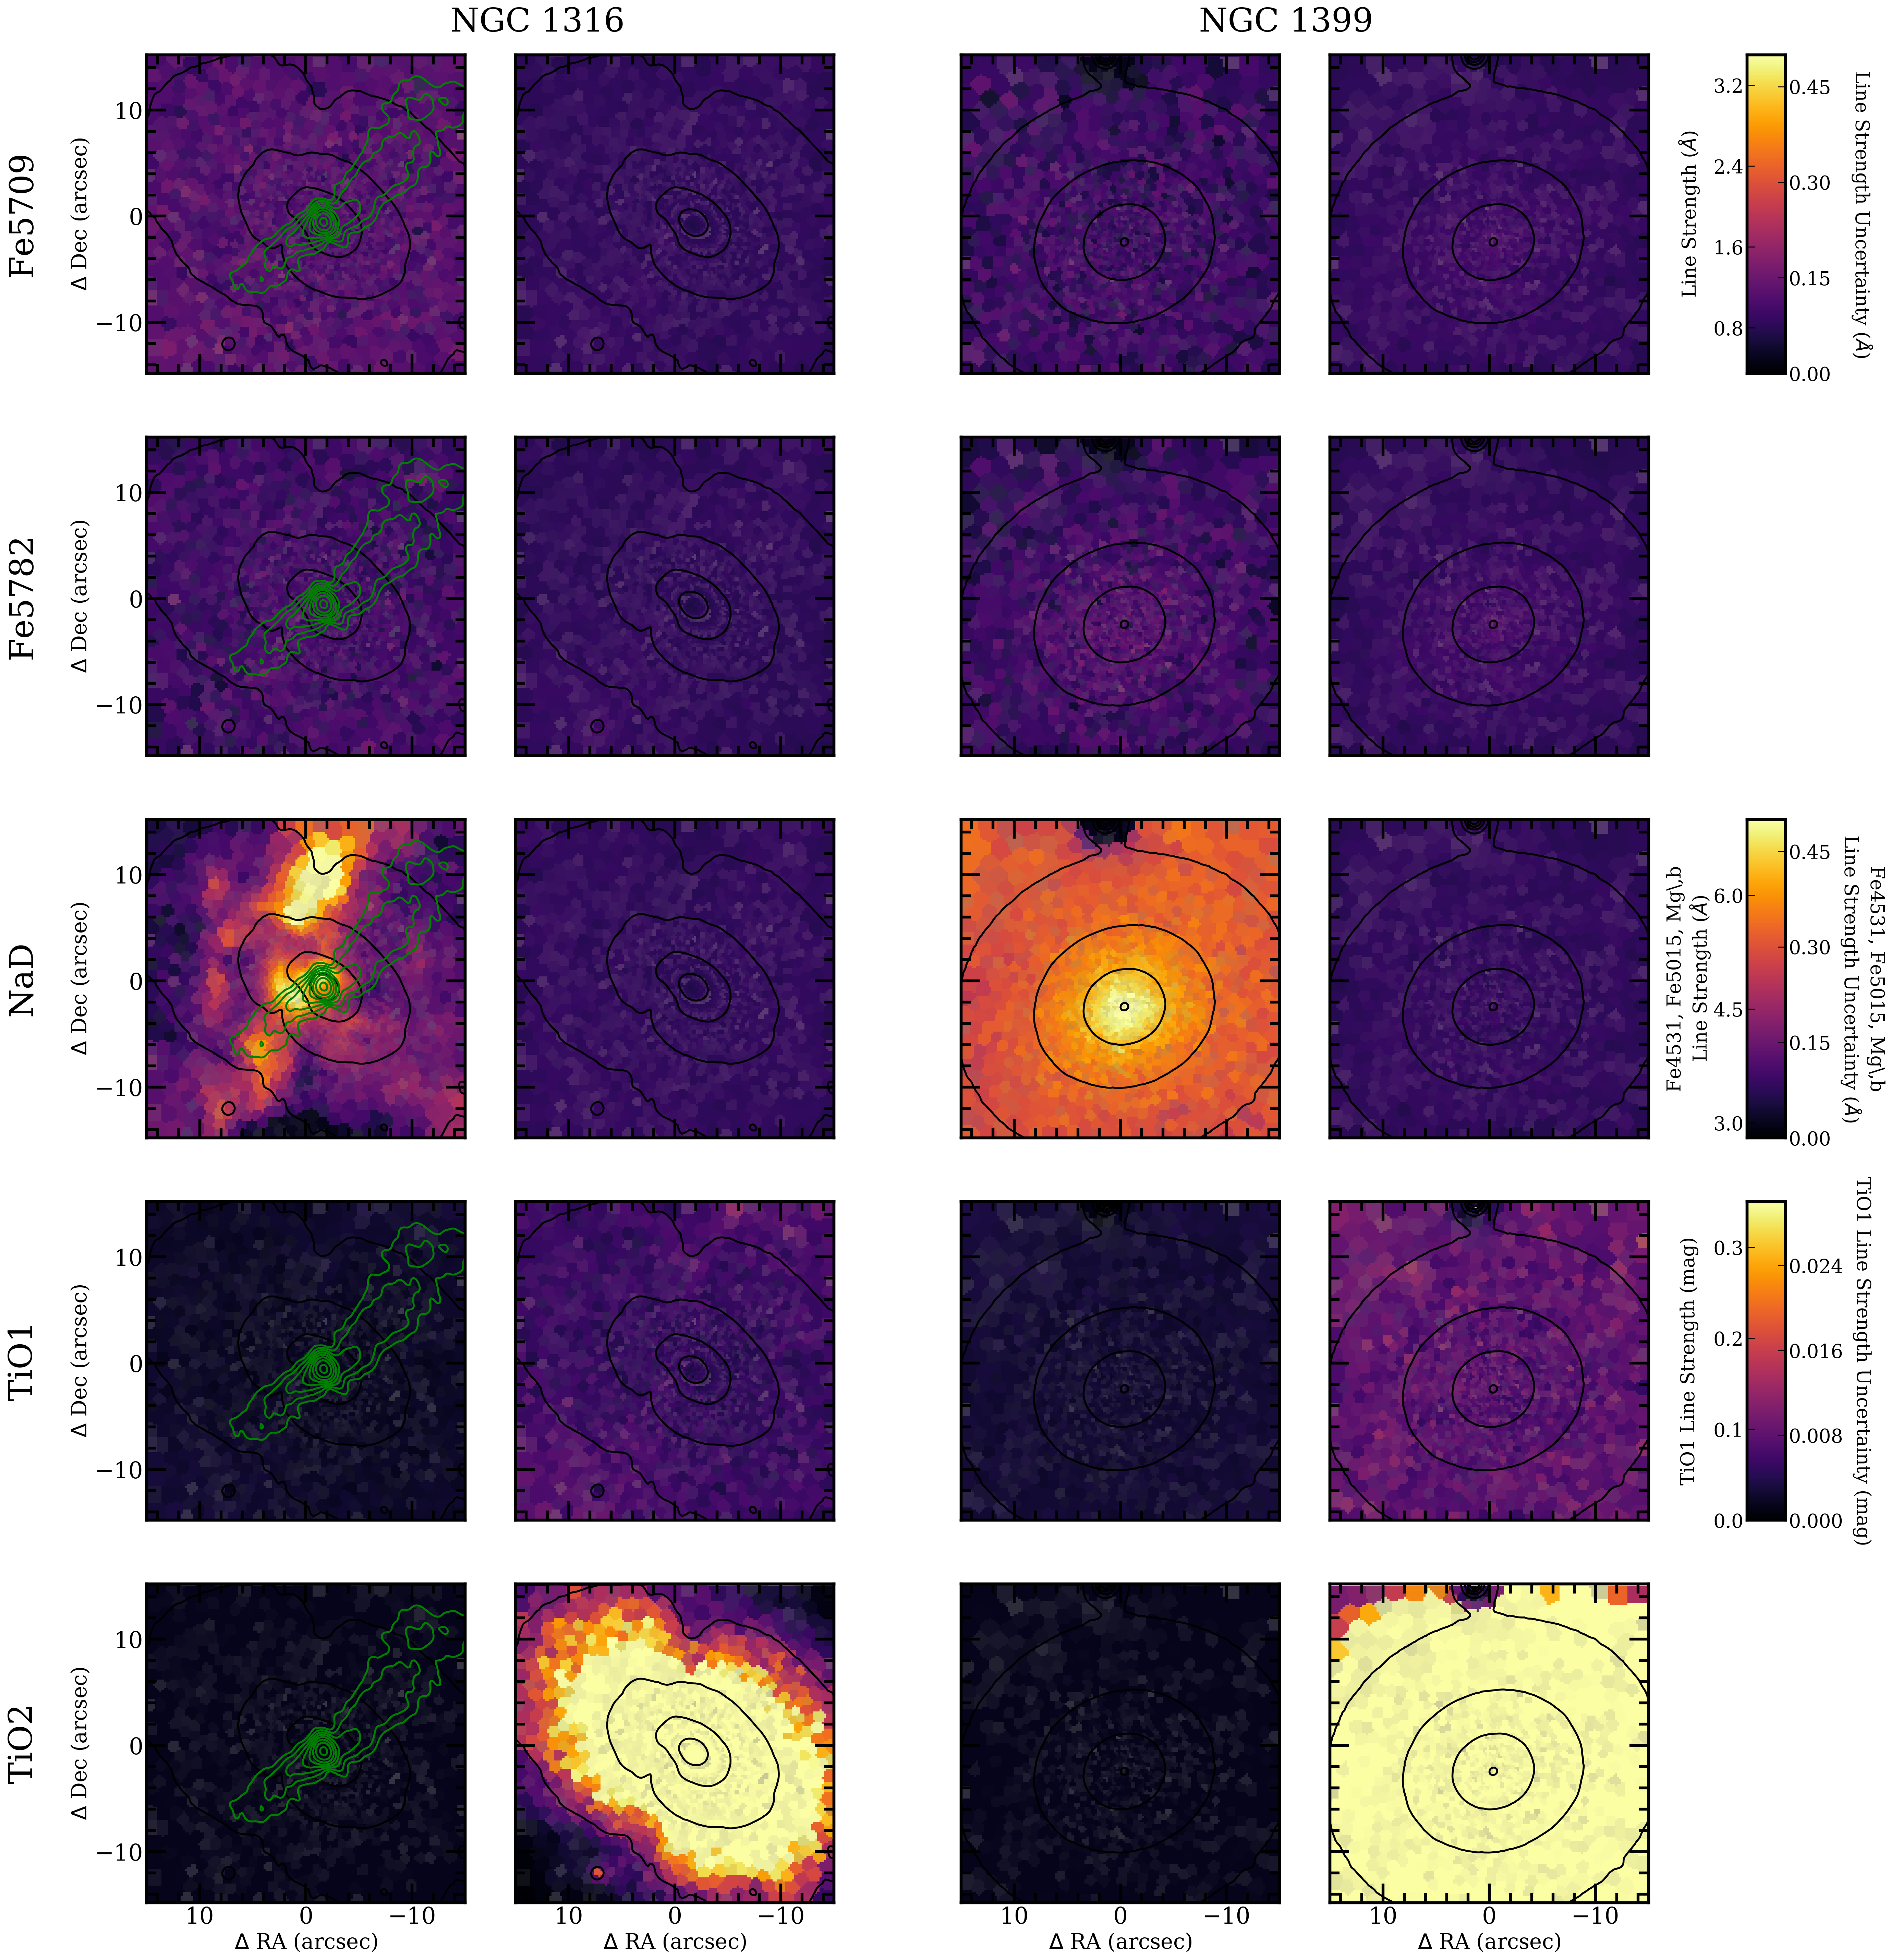
\includegraphics[height=0.54\textheight]{chapter4/muse/abs2b.png}
			\contcaption{continued for NGC1316 and NGC1399.}
		\end{figure*}


	Comparisons to the literature is made difficult by the inhomogeneous nature of corrections applied: such as accounting for H$_\beta$ emission or velocity dispersion. We use Line Index System (LIS) by \citet{Vazdekis2010} instead of the popular LICK/IDS system \citep{Faber1985, Worthey1994} as LICK/IDS is based on non-flux calibrated spectra from the IDS and Cassegrain spectrograph on the Shane telescope (Lick Observatory) which has a relatively low and wavelength dependent resolution. In order to make calibrate measurements from other instruments it is necessary to perform empirical corrections to correct for the uncalibrated continuum. This requires observing standard stars with the same instrumental set up as the main observations in order to make comparisons to the measurements from the IDS spectrograph. Since this was not requested as part of the observing strategy with VIMOS we were not able to do this: a later proposal would not have worked since VIMOS was substantially upgraded in the intervening time period. Further more, we believe that this system has had its time and the community should be making a concerted effort to move away from it, due to the low resolution and poor data quality on which it is based. However, there is a lack of non-LICK/IDS system measurements: we used the empirical functions provided by \citet{Vazdekis2010} to translate between LICK/IDS and LIS systems\footnote{The transformation from LICK/IDS to the LIS system is available at http://www.iac.es/proyecto/miles/pages/line-index-system-lis/transformations.php.}. 


	Finally, we noticed that only the H$_\beta$ emission line is corrected for in some of the literature, despite [OIII] often being the strongest emission line for ETGs. This effects the reliability of the Fe5015 and Mb$_b$ absorption indices as the [OIII] and [NI] doublets fall within them respectively. They vary as to whether they fall within the index band or the continuum bands and the effect depends on the relative difference in the kinematics for the stars (which result in the absorption features) and the ISM (which results in the emission lines). Other papers correct for only H$_\beta$ and [OIII]. In order to make accurate comparisons to the literature we mimic the corrections in the relevant paper for the comparison only including which emission lines they correct for and aperture corrections), while removing all emission lines (given in table \ref{}) for our quoted measurements and maps. Table \ref{tab:litAbsorption} sums up our comparisons to the literature. Here we note that in the case of comparisons to \citet{Rampazzo2005}, G4300 has a very large offset. We suggest that this index is extremely sensitive to the velocity dispersion due to the steep nature of the pseudo-continuum: a difference of $30 \mathrm{km \, s^{-1}}$ can effect the corrected index value by $\sim 2$\AA. For the comparison to \citet{Vazdekis2010}, we analyzed the SAURON data set\footnote{SARUON data is available at: http://www.strw.leidenuniv.nl/sauron/} \citep{Emsellem2004} using the same pipeline we have developed for our sample. 

	% Could use another paper to compare to: Orgando? 
	\begin{table}
		\centering
		\caption{Comparisons to the literature. Comparisons to \citet{Rampazzo2005} are sampled at 7 radial apertures for each galaxy: 1.5, 2.5 and 10.0 arcsec and R$_e$/10, R$_e$/8, R$_e$/4 and R$_e$/2. Offset is the mean difference between our measurements and that of the literature, while Dispersion is the standard deviation of the difference.}
		\label{tab:litAbsorption}
		\begin{tabular}{l r r r}
			\hline
			\hline
			Index 		& N$_{gals}$ & Offset 	& Dispersion \\
						& 			& $\AA$		& $\AA$ \\
			\hline
			\multicolumn{4}{c}{\citet{Vazdekis2010} (SAURON)} \\
			\hline
			H$_\beta$ 	& 46		& -0.02		& 0.25	\\
			Fe5015		& 46		& 0.66		& 0.34	\\
			Mg$_b$ 		& 46		& 0.06		& 0.33	\\
			\hline
			\multicolumn{4}{c}{\citet{Rampazzo2005} (VIMOS)} \\
			\hline
			G4300 		& 3 		& 2.29		& 0.11	\\
			Fe4383 		& 3 		& 0.39		& 0.23	\\
			Ca4455 		& 3 		& -0.19		& 0.09	\\
			Fe4531 		& 3 		& 0.16		& 0.26	\\
			H$_\beta$ 	& 3 		& 0.17		& 0.12	\\
			Fe5015 		& 3 		& -0.73		& 0.48	\\
			Mg$_b$ 		& 3 		& -0.43		& 0.17	\\
			\hline
			\multicolumn{4}{c}{\citet{Rampazzo2005} (MUSE)} \\
			\hline
			H$_\beta$ 	& 2 		& -0.28		& 0.17	\\ 
			Fe5015 		& 2 		& 0.87		& 0.34	\\ 
			Mg$_b$ 		& 2 		& 0.31		& 0.14	\\
			Fe5270 		& 2 		& -0.11		& 0.15	\\
			Fe5335 		& 2 		& 0.08		& 0.15	\\
			Fe5406 		& 2 		& 0.16		& 0.07	\\
			Fe5709 		& 2 		& 0.11		& 0.10	\\
			Fe5782 		& 2 		& -0.03		& 0.11	\\
			NaD 		& 2 		& 0.90		& 0.41	\\
			TiO1 (mag)	& 2 		& -0.004	& 0.003	\\
			TiO2 (mag)	& 2 		& -0.011	& 0.007	\\
			\hline
			\multicolumn{4}{c}{\citet{Ogando2008} (VIMOS)} \\
			\hline
			H$_\beta$ 	& 6 		& 0.07		& 0.60	\\
			Fe5015 		& 6 		& -0.09		& 0.15	\\
			Mg$_b$ 		& 6 		& -0.70		& 0.08	\\
			\hline
			\multicolumn{4}{c}{\citet{Ogando2008} (MUSE)} \\
			\hline
			H$_\beta$ 	& 3 		& -0.04		& 0.23	\\ 
			Fe5015 		& 3 		& -0.16		& 0.33	\\ 
			Mg$_b$ 		& 3 		& -1.10		& 0.26	\\
			Fe5270 		& 3 		& -0.66		& 0.16	\\
			Fe5335 		& 3 		& -0.66		& 0.11	\\
			Fe5406 		& 3 		& -0.51		& 0.06	\\
			Fe5709 		& 3 		& -0.22		& 0.08	\\
			NaD 		& 3 		& -1.57		& 0.16	\\
			%[OIII]5007	& 3 		& 		& 	\\
			\hline
		\end{tabular}
	\end{table}

	% \subsection{Gradients in absorption line strengths}
	% 	\label{subsec:absorptionGrad}


	\subsection{Most-likely stellar population model}
		\label{subsec:ssp}
		Using the method described in section \ref{} we found the most-likely simple stellar population (SSP) characteristics: age (t), metallicity (Z) and alpha enhancement (\textalpha); by comparing our measured absorption line indices to that of models. We first give an overview of the process of generating synthetic stellar populations before detailing the specifics of the models used below. 

		Synthetic SSPs are created by starting using the following ingredients:
		\begin{itemize}
			\item the loci of a star of a given mass and metallicity, as they travel across the Hertzsprung--Russel Diagram (HRD) by aging. These are known as stellar evolutionary tracks and are generally empirical.
			\item  the function representing the number of stars of a given mass, $N(M)$, at formation ($t = 0$). This is the initial mass function (IMF).
			\item an empirical library of stellar spectra to be able to assign a a spectra to a position on the HRD. 
		\end{itemize}
		% The SSP spectra $S(t,Z)$ can be parameterized as an integral over the masses, M,:
		% \begin{equation}
		% 	S(t,Z) = \int \! \Phi(M) \Lambda[L(M,Z,t), T(M,Z,t),Z] \,\mathrm{d}M
		% \end{equation}
		% where $\Phi$ is the IMF and $\Lambda$ is the stellar spectra, which is characterized by the luminosity (L), temperature (T) and metallicity. 
		The desired output of expected index strengths on a 3D grid of varying age, metallicity and alpha enhancement can be computed in one of two ways: (i) produce full synthetic spectra from the evolution of stellar atmospheres or (ii) find a 'fitting function' for each index which analytically calibrate the index strengths measured from empirical libraries to physical stellar parameters. The former is dependent on a good understanding of the physics of stellar atmospheres and is known to suffer from incomplete line lists and continuum uncertainties \citep{Thomas2004}. The later, and by far the more popular method, allows interpolation between well populated regions of the parameter space which helps to (a) compute the uncertainties in the model predictions and (b) decrease those uncertainties in sparse regions of the parameter space. 

		ETGs may have very different fractional abundances of various metals to the nearby stars that we are able to observe (all of which have solar or very near solar abundances). As such the stellar libraries that are used to calibrate the models fall far short of the required coverage of the parameter space. Most methods make some effort to extrapolate to non-solar abundances. In a similar way to the fitting functions described above, 'index response functions' can be found to calibrate the effect of varying the abundances of individual elements, though here, comparisons must be with completely theoretical spectra.

		We used the models from \citet{Thomas2010} (referred to hereafter as the TMJ models) because they have the novelty of being based on flux calibrated spectra and hence do not need observations to be calibrated to the LICK/IDS system. These models assume a \citet{Salpeter1955} IMF ($\Phi(M) \equiv \frac{\mathrm{d}N(M)}{\mathrm{d}M} \propto M^{-2.35}$) and are based on the evolutionary population synthesis code from \citet{Maraston1998}. This uses the stellar evolutionary tracks from \citet{Cassisi1997} for metallicities of [Z/H] < -0.33 and \citet{Girardi2000} for [Z/H] $\ge -0.33$, the MILES stellar spectral library from \citet{Sanchez-Blazquez2006a, Falcon-Barroso2011a}, fitting functions from \citet{Johansson2010} and index response functions from \citet{Korn2005}.

		The \citet{Korn2005} response functions extend the work of \citet{Tripicco1995} who investigated the response functions of the original 21 Lick indices to the varying of individual element abundance fractions for 5 Gyr old SSP at solar metallicities. The new functions now include varying metallicities, as well as individual element fractions are calculated for all 25 Lick indices. It was checked whether age has a significant effect on the response functions by computing them for 1 Gyrs models and comparing them to 5 Gyrs models from \citet{Tripicco1995}. They found a 1\% difference for two indices (G4300 and Fe4383) and a significantly lower result for all other indices, showing that age does not effect the response functions.

		Finally, the individual element abundances are combined to give the alpha element enhancement parameter, \textalpha/Fe. This is done following \citet{Trager2000} who grouped the elements into three categories: enhanced, containing C, N, O, Na, Mg, Si, Ca and Ti (i.e. \textalpha and other light elements); depressed, containing Cr and Fe (i.e. iron peak elements); and all other elements are fixed. The fixed group are held with solar abundances, while the enhanced and depressed groups are scaled up and down respectively by the same factor. 

		The TMJ models return index strengths for a 3D grid of models with t = 0.1, 0.2, 0.4, 0.6, 0.8, 1,2, 3,4, 5, 6, 7, 8, 9, 10, 11, 12, 13, 14, 15 \text{Gyrs}; [Z/H] = -2.25, -1.35, -0.33, 0.0, 0.35, 0.67 and [\alpha/Fe] = -0.3, 0.0, 0.3, 0.5.  

		\citet{Thomas2010} shows that the TMJ model gives a good fit to globular cluster measurements of \citet{Puzia2002, Schiavon2005} and the galaxy measurements by the SAURON group in \citet{Kuntschner2010}. \citet{Conroy2010} suggests that the \citet{Girardi2000} tracks used for the high metallicity models does not fit globular clusters well, however \citet{Thomas2010} points out that it is mostly down to an anomaly in the Balmer lines which is not seen in the analysis of the SAURON data. They therefore suggest that it is an issue with the globular cluster observations themselves. 

		Figures \ref{fig:VIMOS_pop} and \ref{fig:MUSE_pop} show the mostly stellar populations for the Southern Sample, assuming that they can reasonably represented by a single stellar population (SSP). In general they show old, metal rich and alpha enhanced SSPs: very typical for ETGs. The exceptions are NGC 612 and NGC 1316. NGC 612 is discussed in more detail in section \ref{sec:NGC612}, while NGC 1316 simply shows a very young stellar population (our fit agrees with that of \citet{Kuntschner2000}, but is conflicting with the older (4.7 Gyr) and less metal rich ([Fe/H]$ = 0.07$) stellar population found by \citet{Koleva2011}). 

		Some ideas around the fueling of the AGN suggest that star formation would play a role in modulating the flow of gas into the central black hole \citep{}, and while it would be expected to be small in scale, spatially, we might reasonably expect a young SSP to dominate in the very central (1-2) spaxels. We note that these maps show no evidence of this. 

	\begin{figure*}
		\centering
		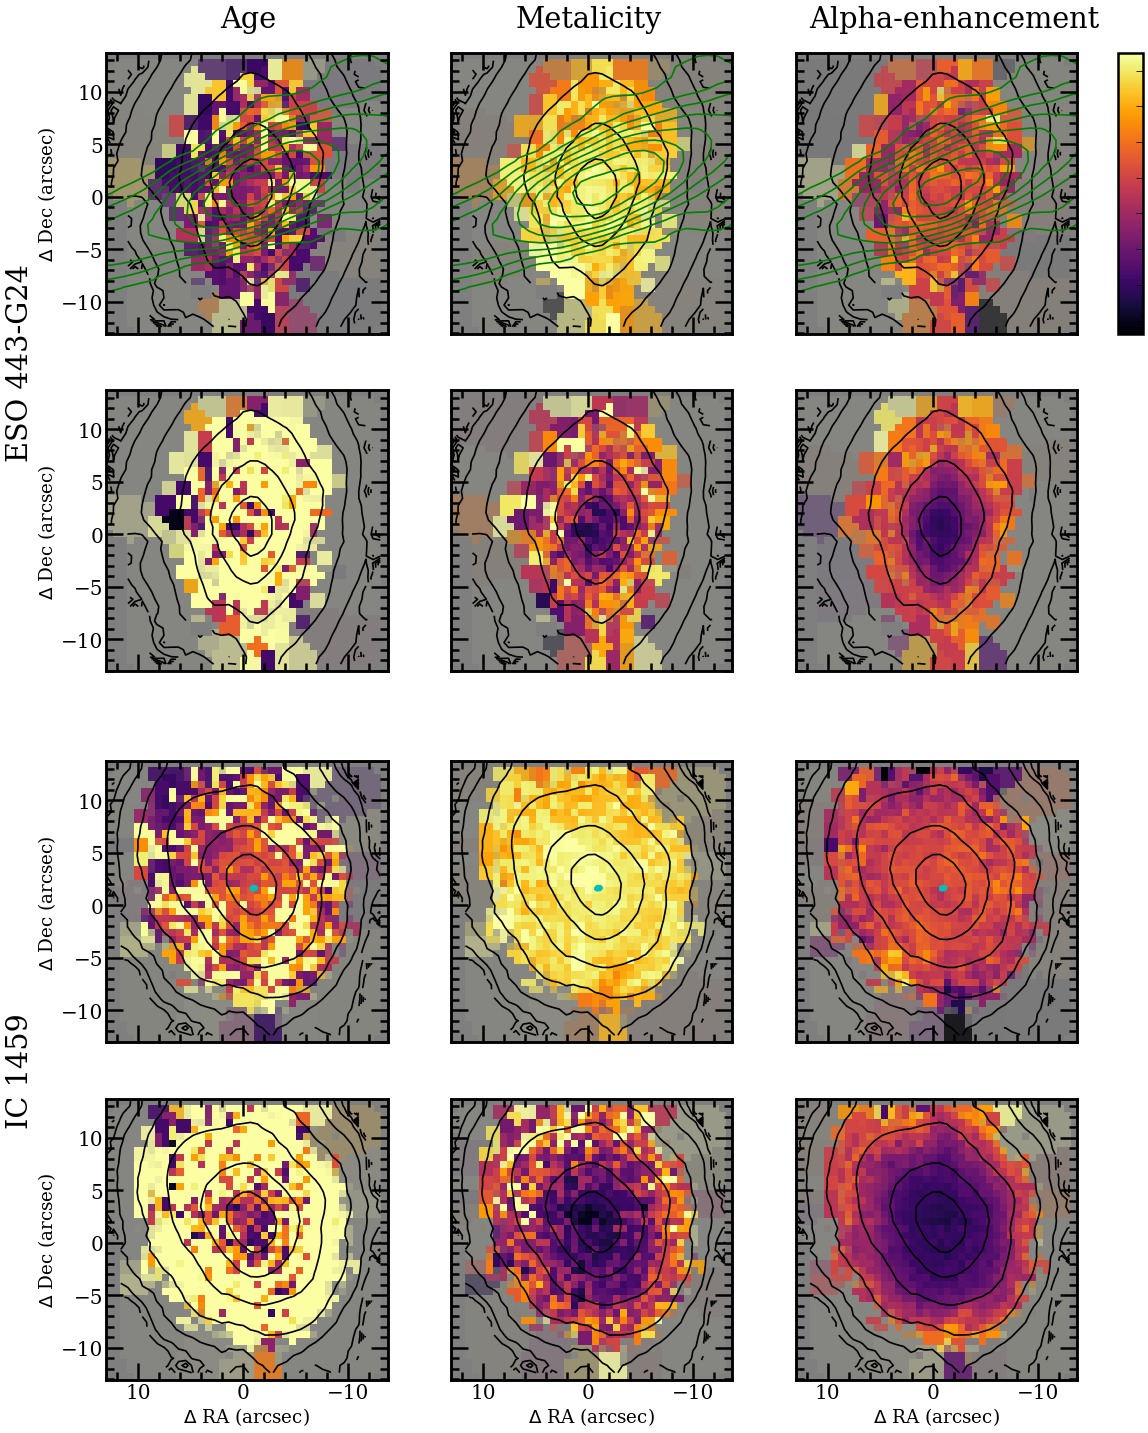
\includegraphics[height=0.94\textheight]{chapter4/vimos/pop1.png}
		\caption[VIMOS stellar population maps]{VIMOS stellar population maps: From left to right: age, metallicity and alpha enhancement, Top to bottom ESO 443-G24, IC 1459 and IC 1531. Rows show parameter and uncertainty in the parameter on alternate rows. Plots are as in figure \ref{fig:VIMOS_stellar}}
		\label{fig:VIMOS_pop}
	\end{figure*}
	\begin{figure*}
		\centering
		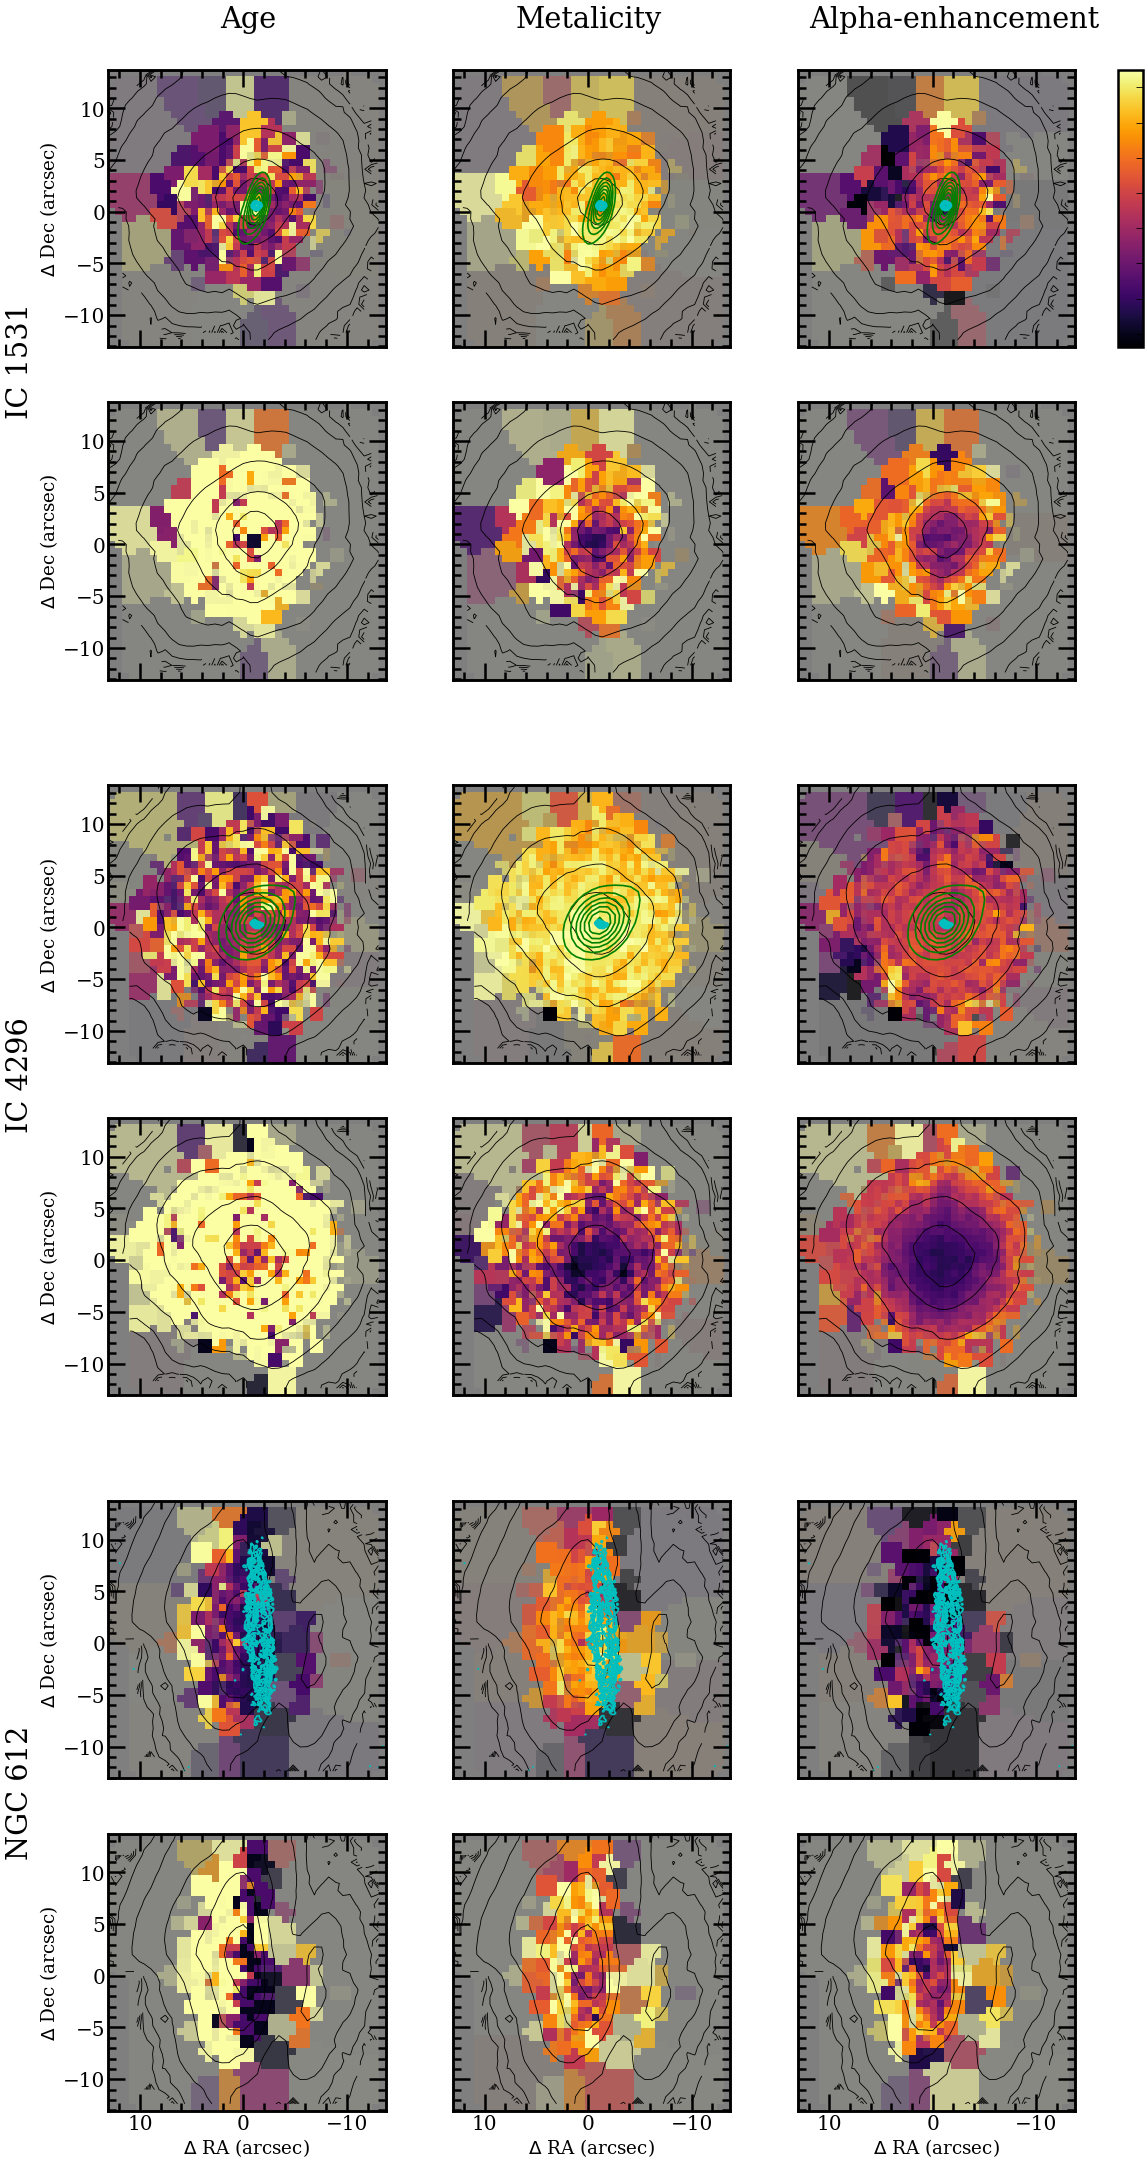
\includegraphics[height=0.94\textheight]{chapter4/vimos/pop2.png}
		\contcaption{continued for IC 4296, NGC 612 and NGC 1399}
	\end{figure*}
	\begin{figure*}
		\centering
		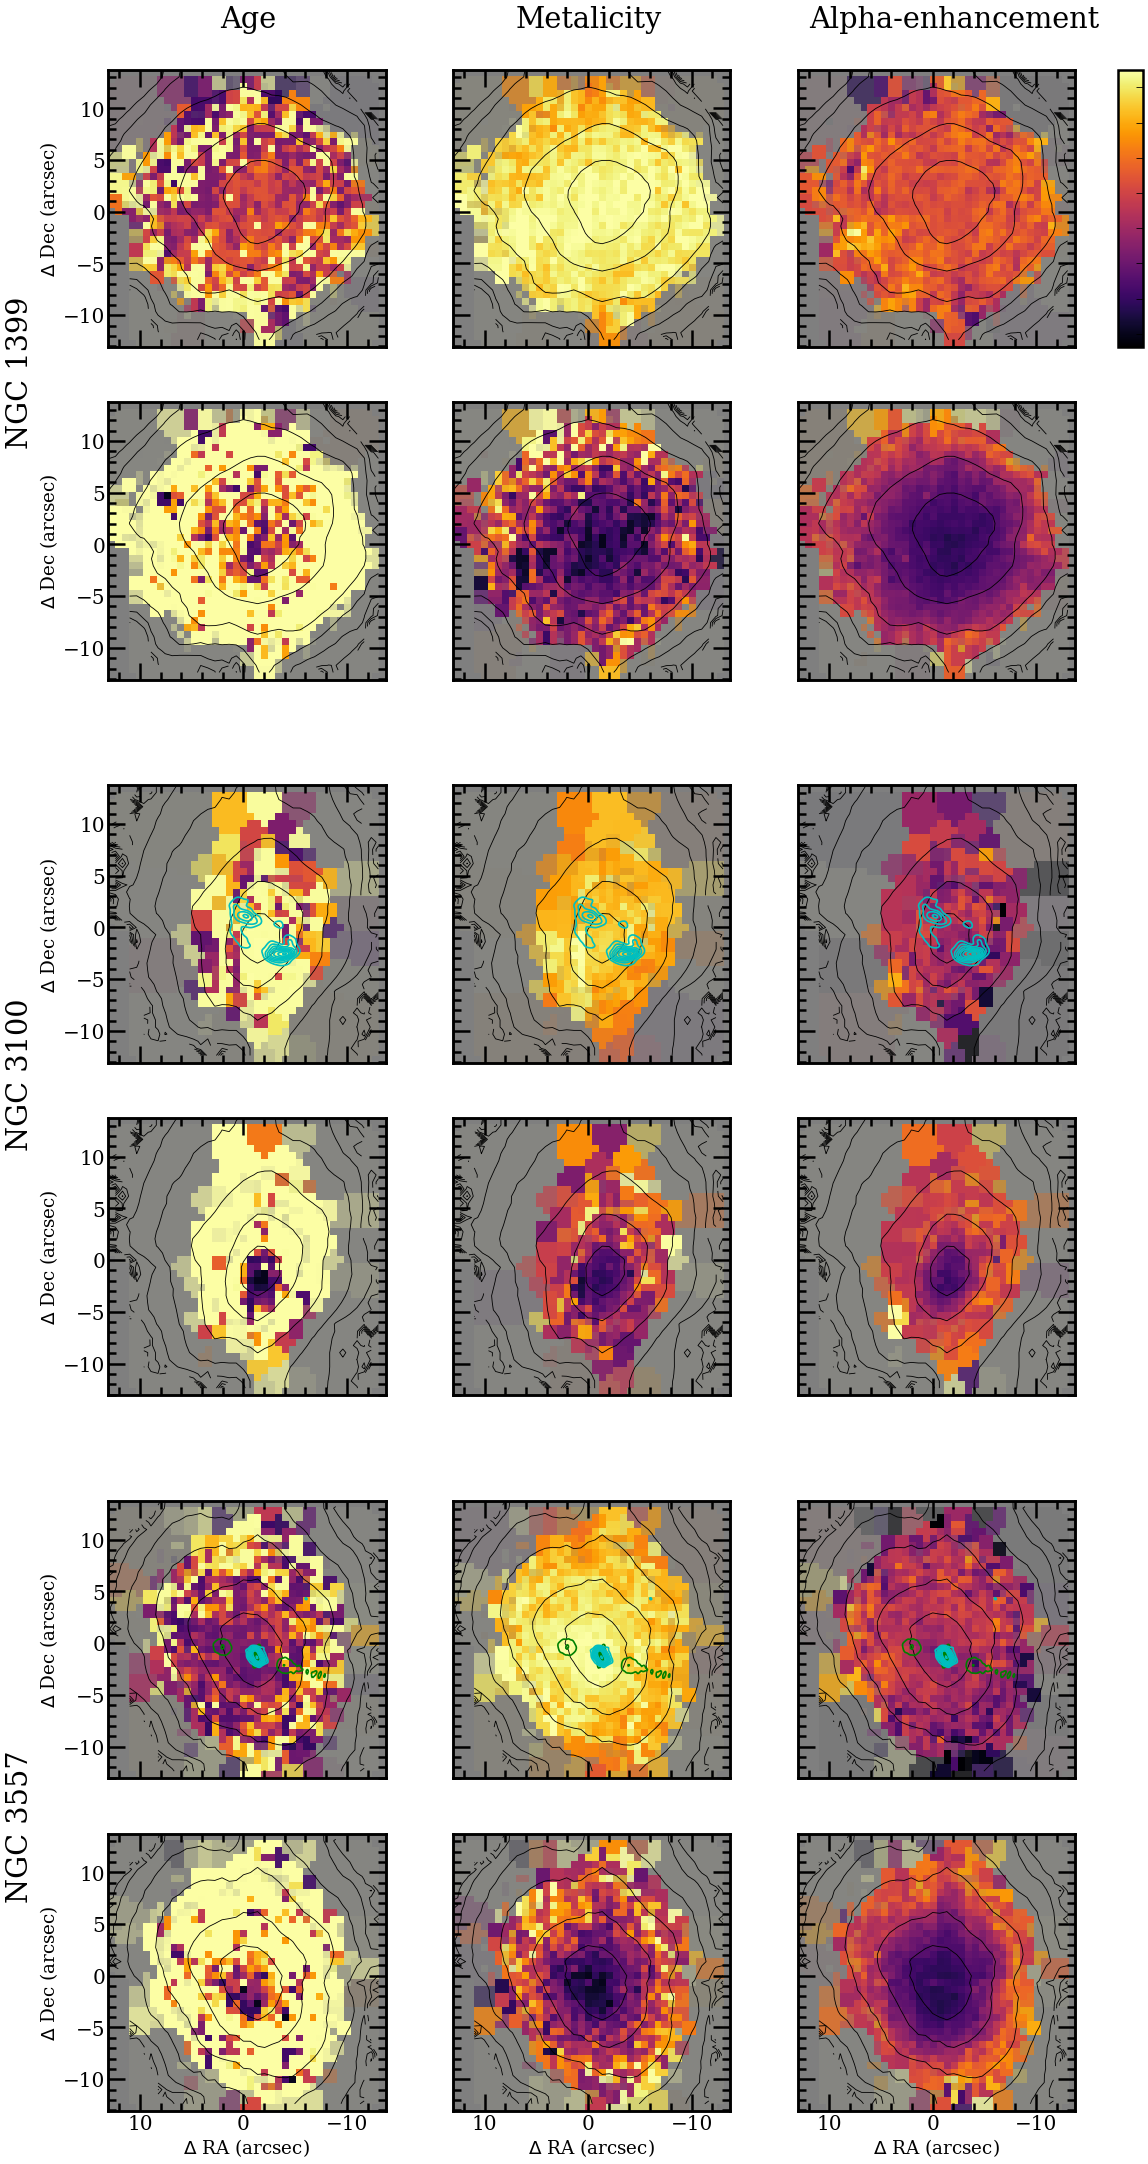
\includegraphics[height=0.94\textheight]{chapter4/vimos/pop3.png}
		\contcaption{continued for NGC 3100, NGC 3557 and NGC 7075}
	\end{figure*}
	\begin{figure*}
		\centering
		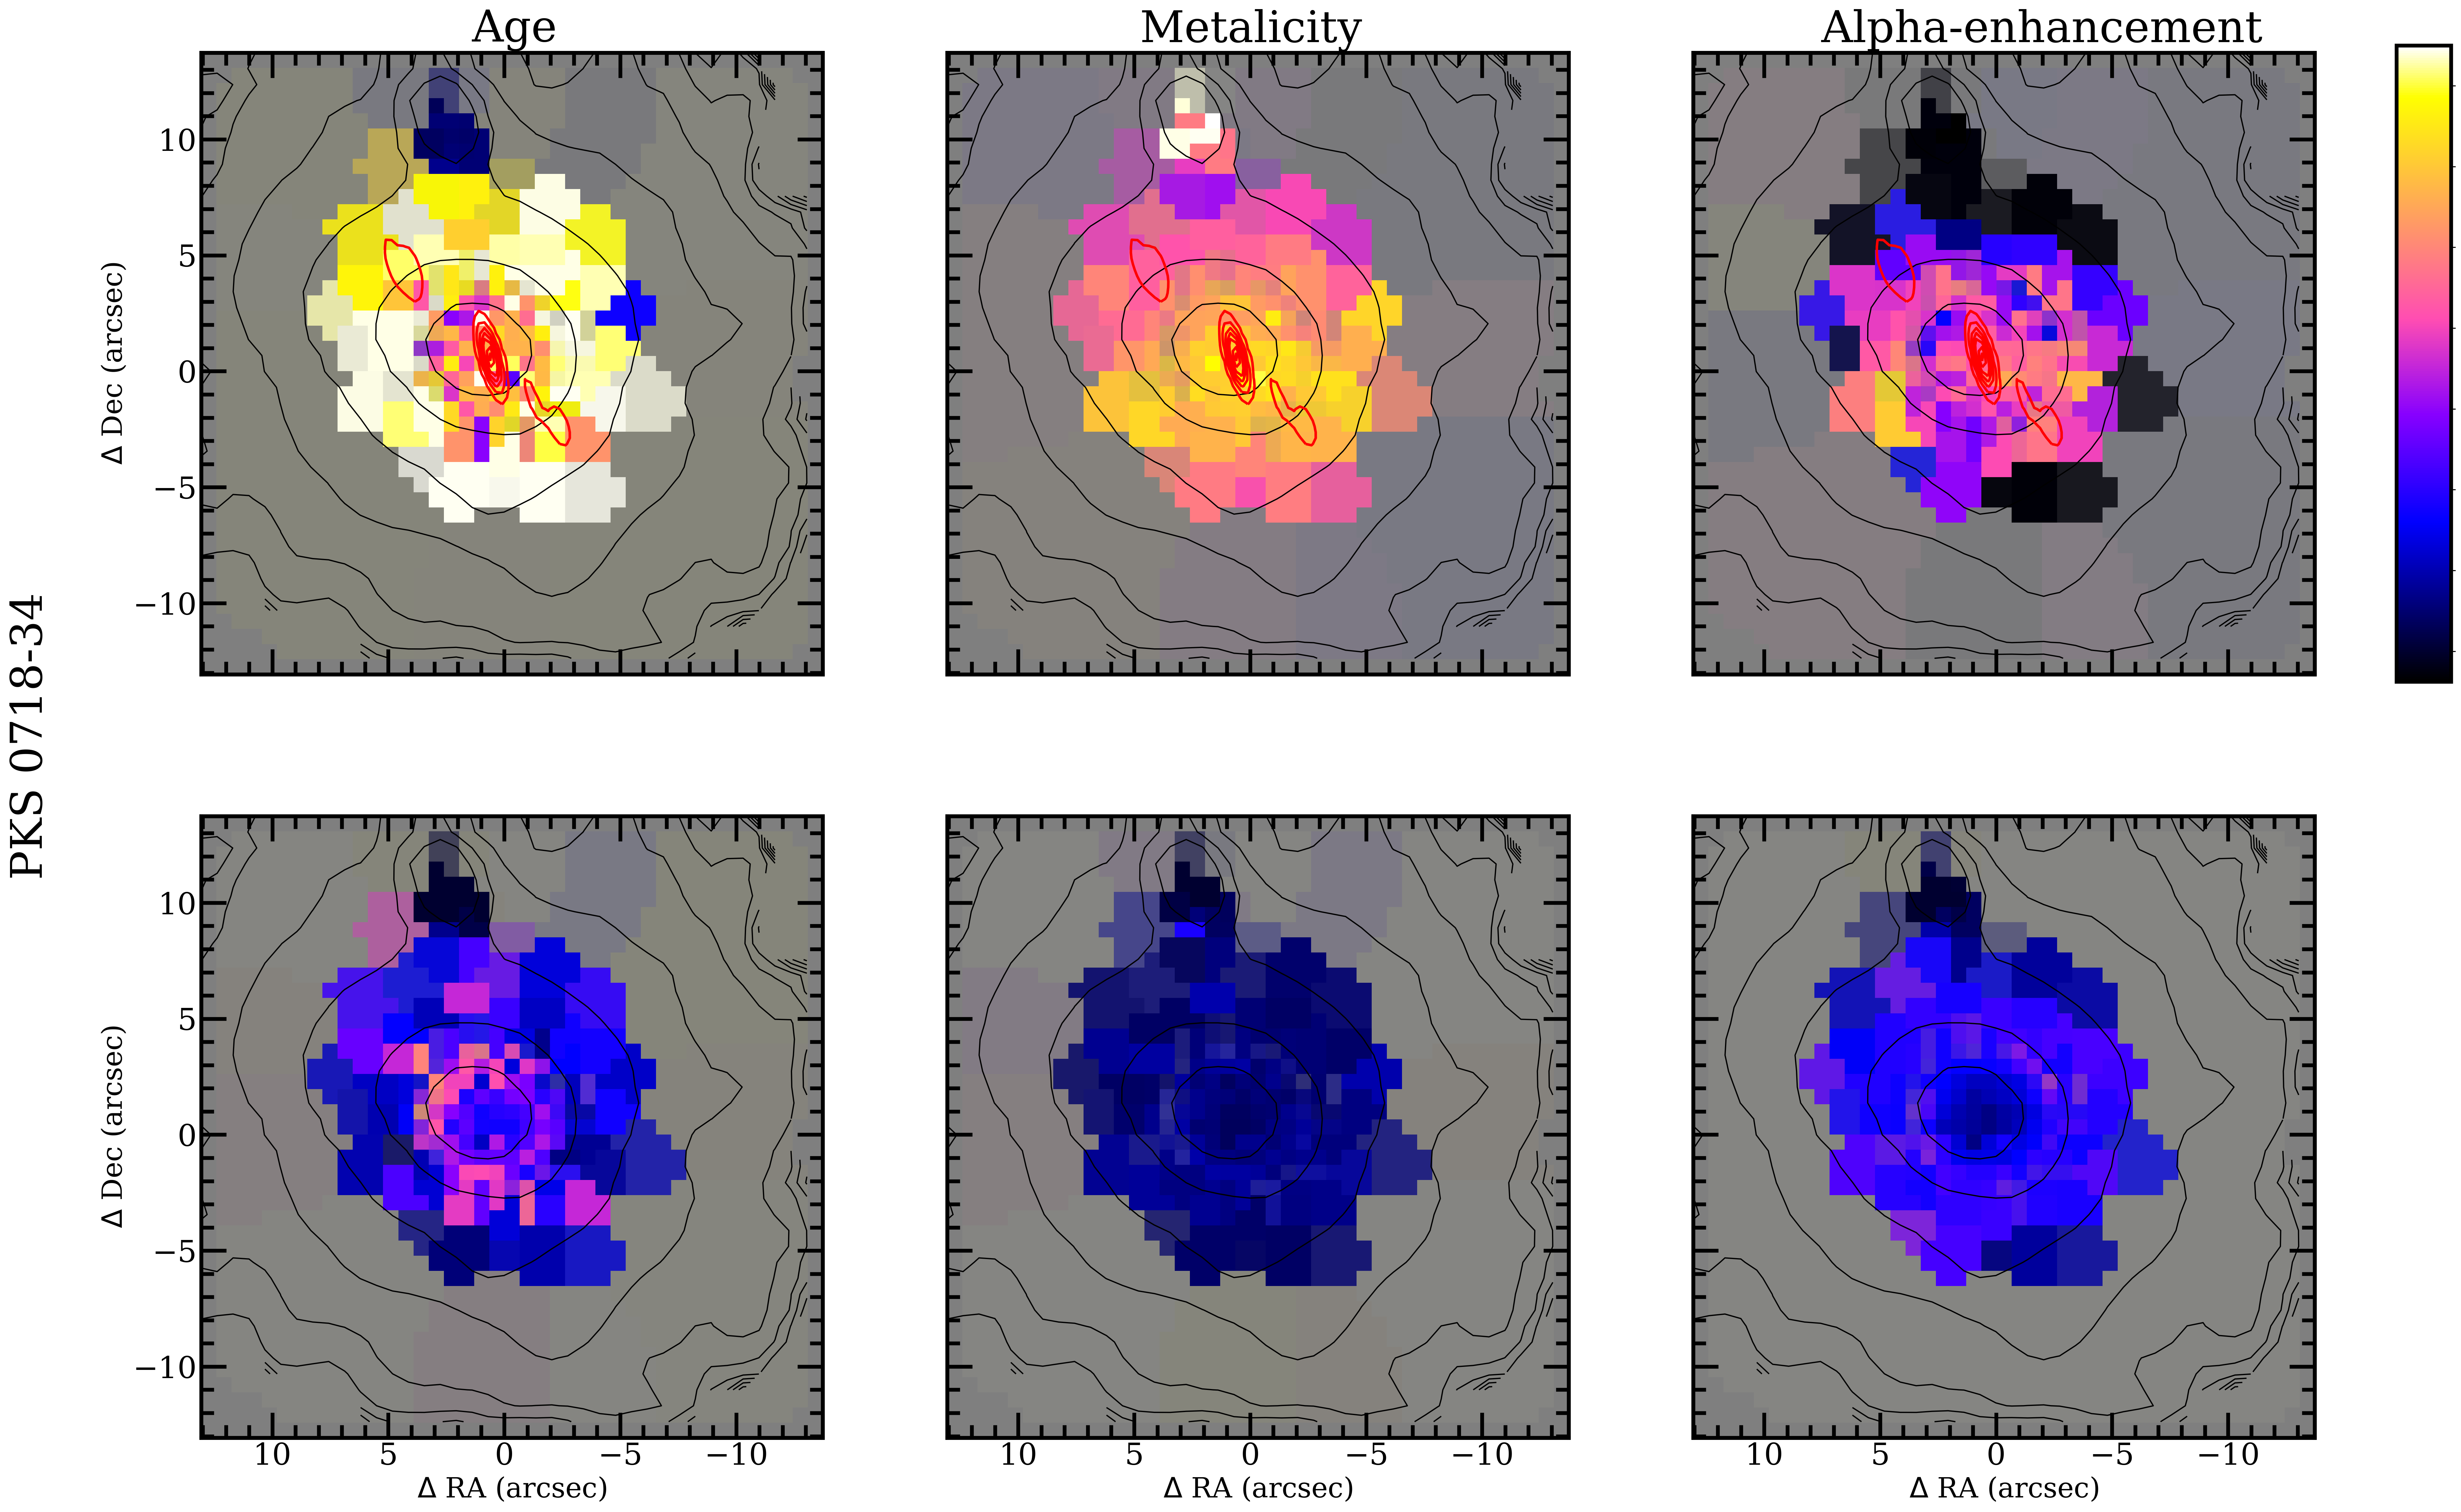
\includegraphics[height=0.31\textheight]{chapter4/vimos/pop4.png}
		\contcaption{continued for PKS 718-34}
	\end{figure*}

	\begin{figure*}
		\centering
		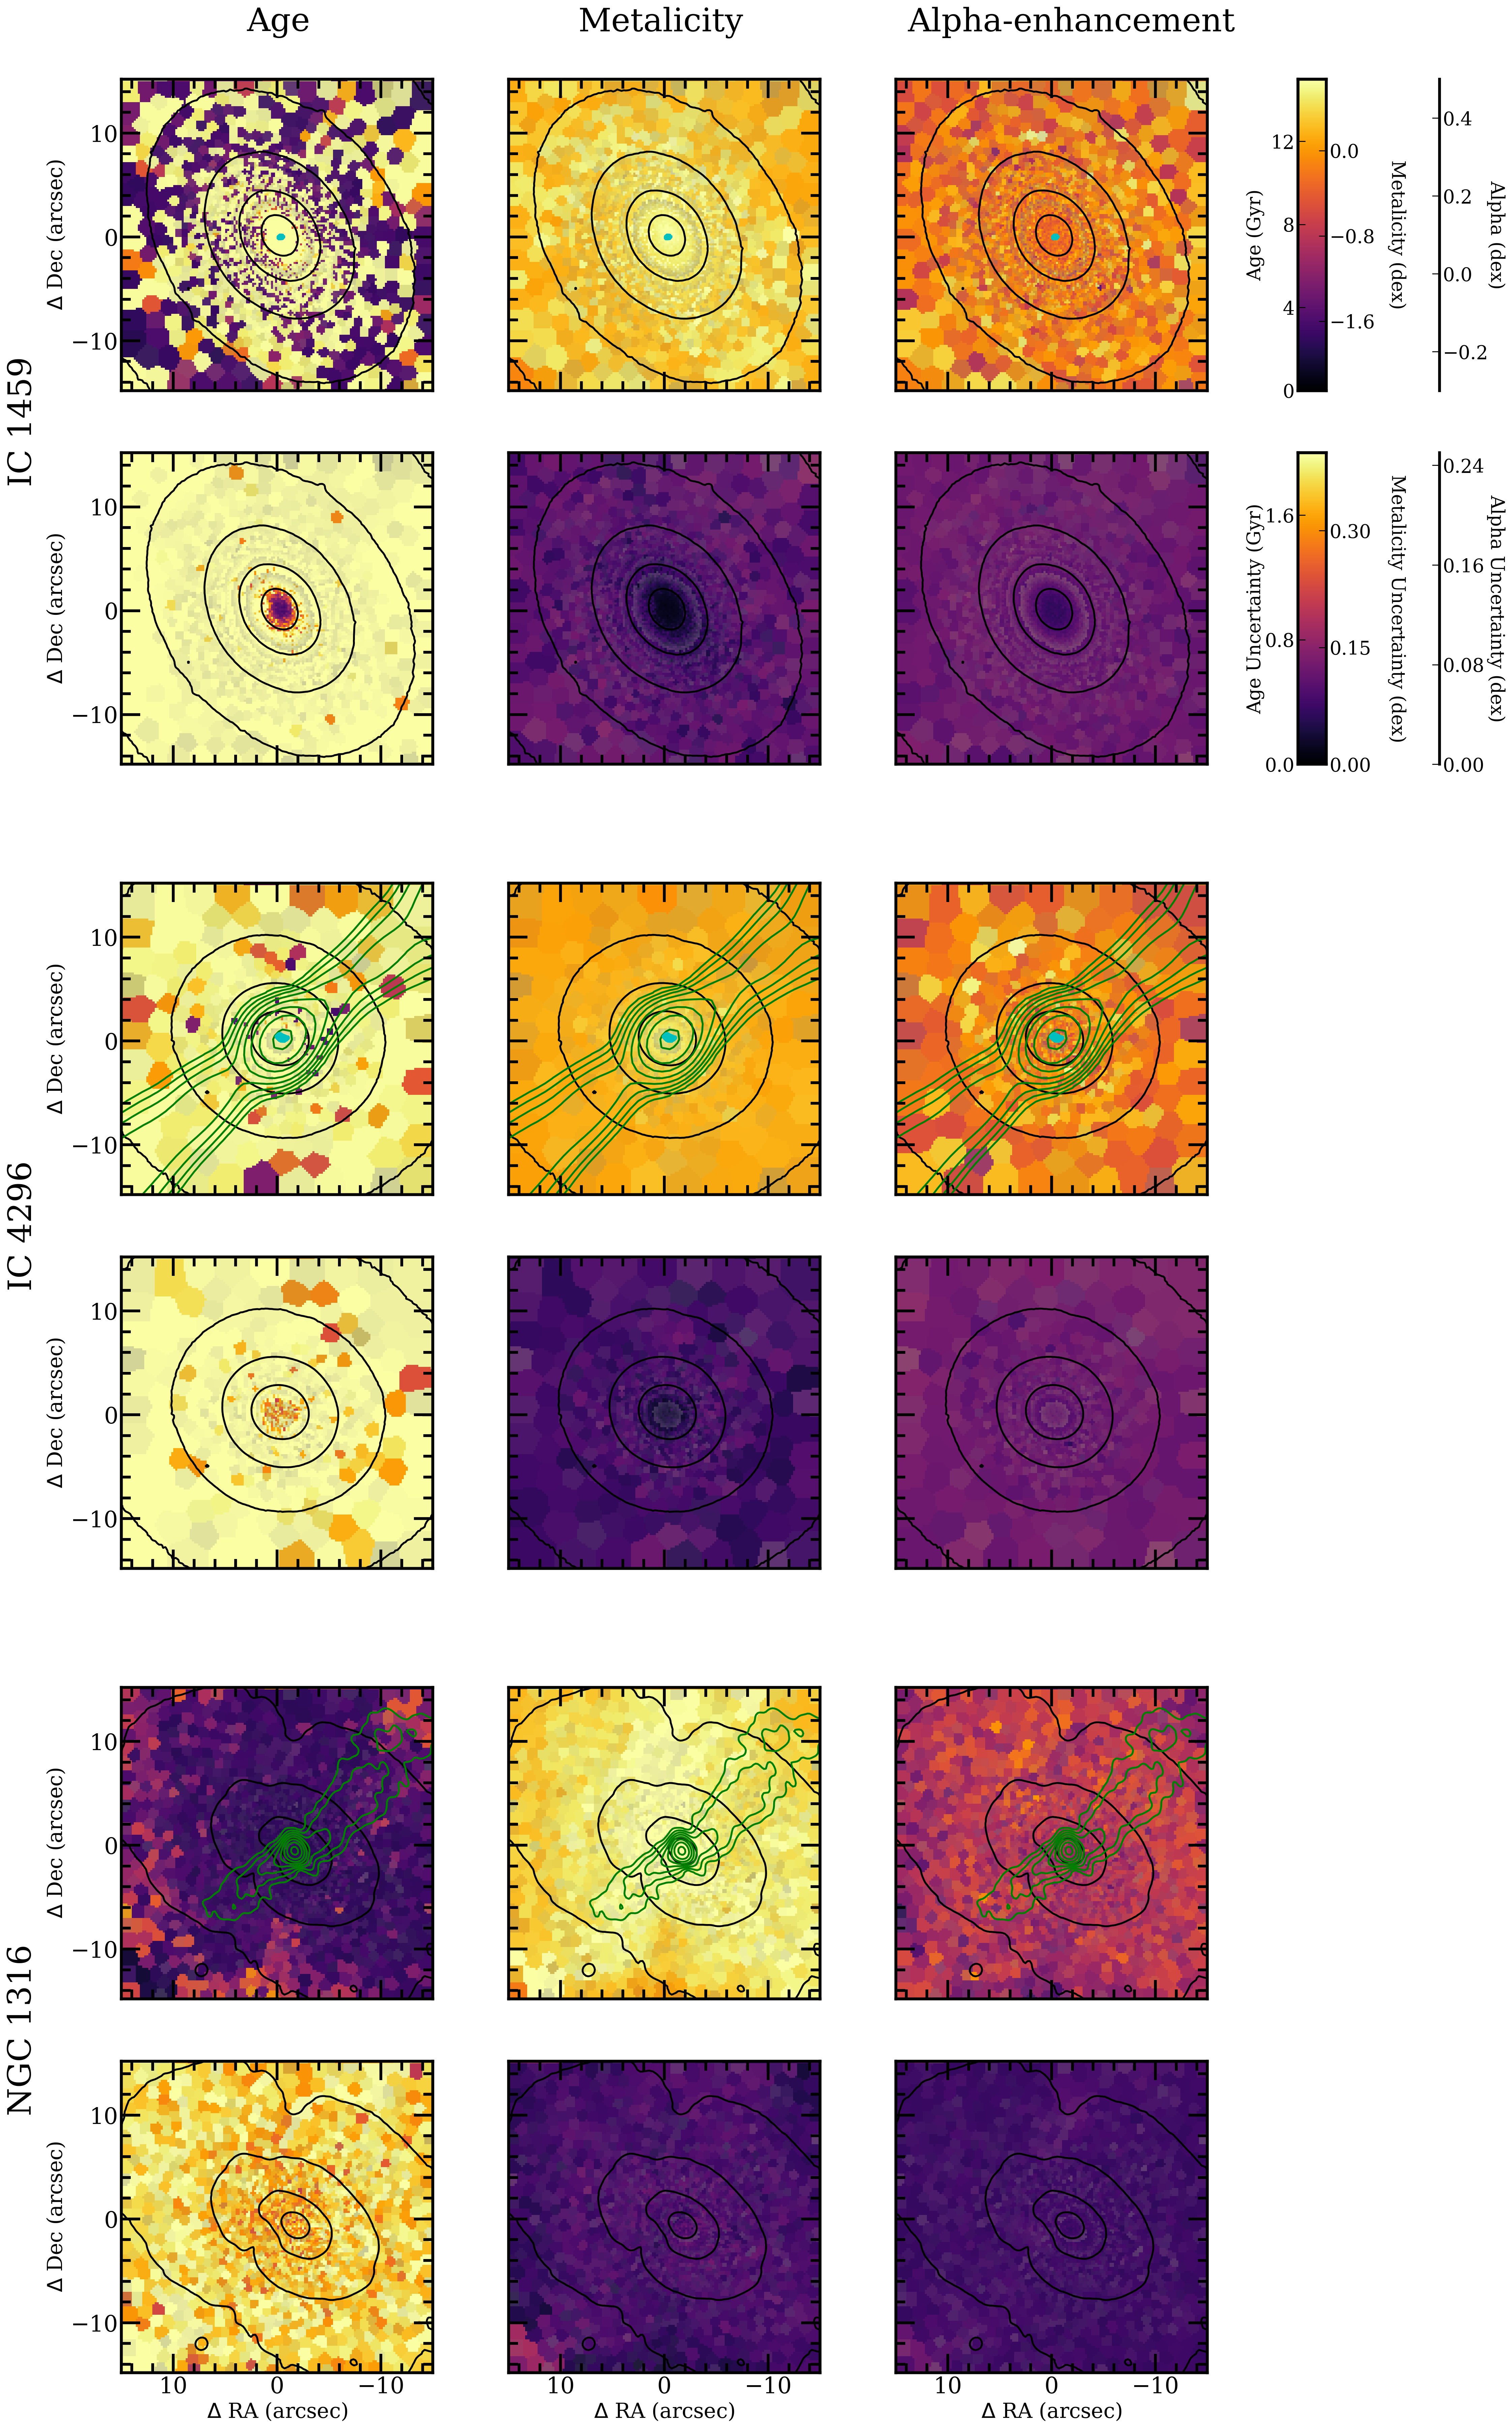
\includegraphics[height=0.94\textheight]{chapter4/muse/pop1.png}
		\caption[MUSE stellar population maps]{MUSE stellar population maps: From top to bottom IC 1459, IC 4296 and NGC 1316. Plots are as in figure \ref{fig:VIMOS_stellar}}
		\label{fig:MUSE_pop}
	\end{figure*}
	\begin{figure*}
		\centering
		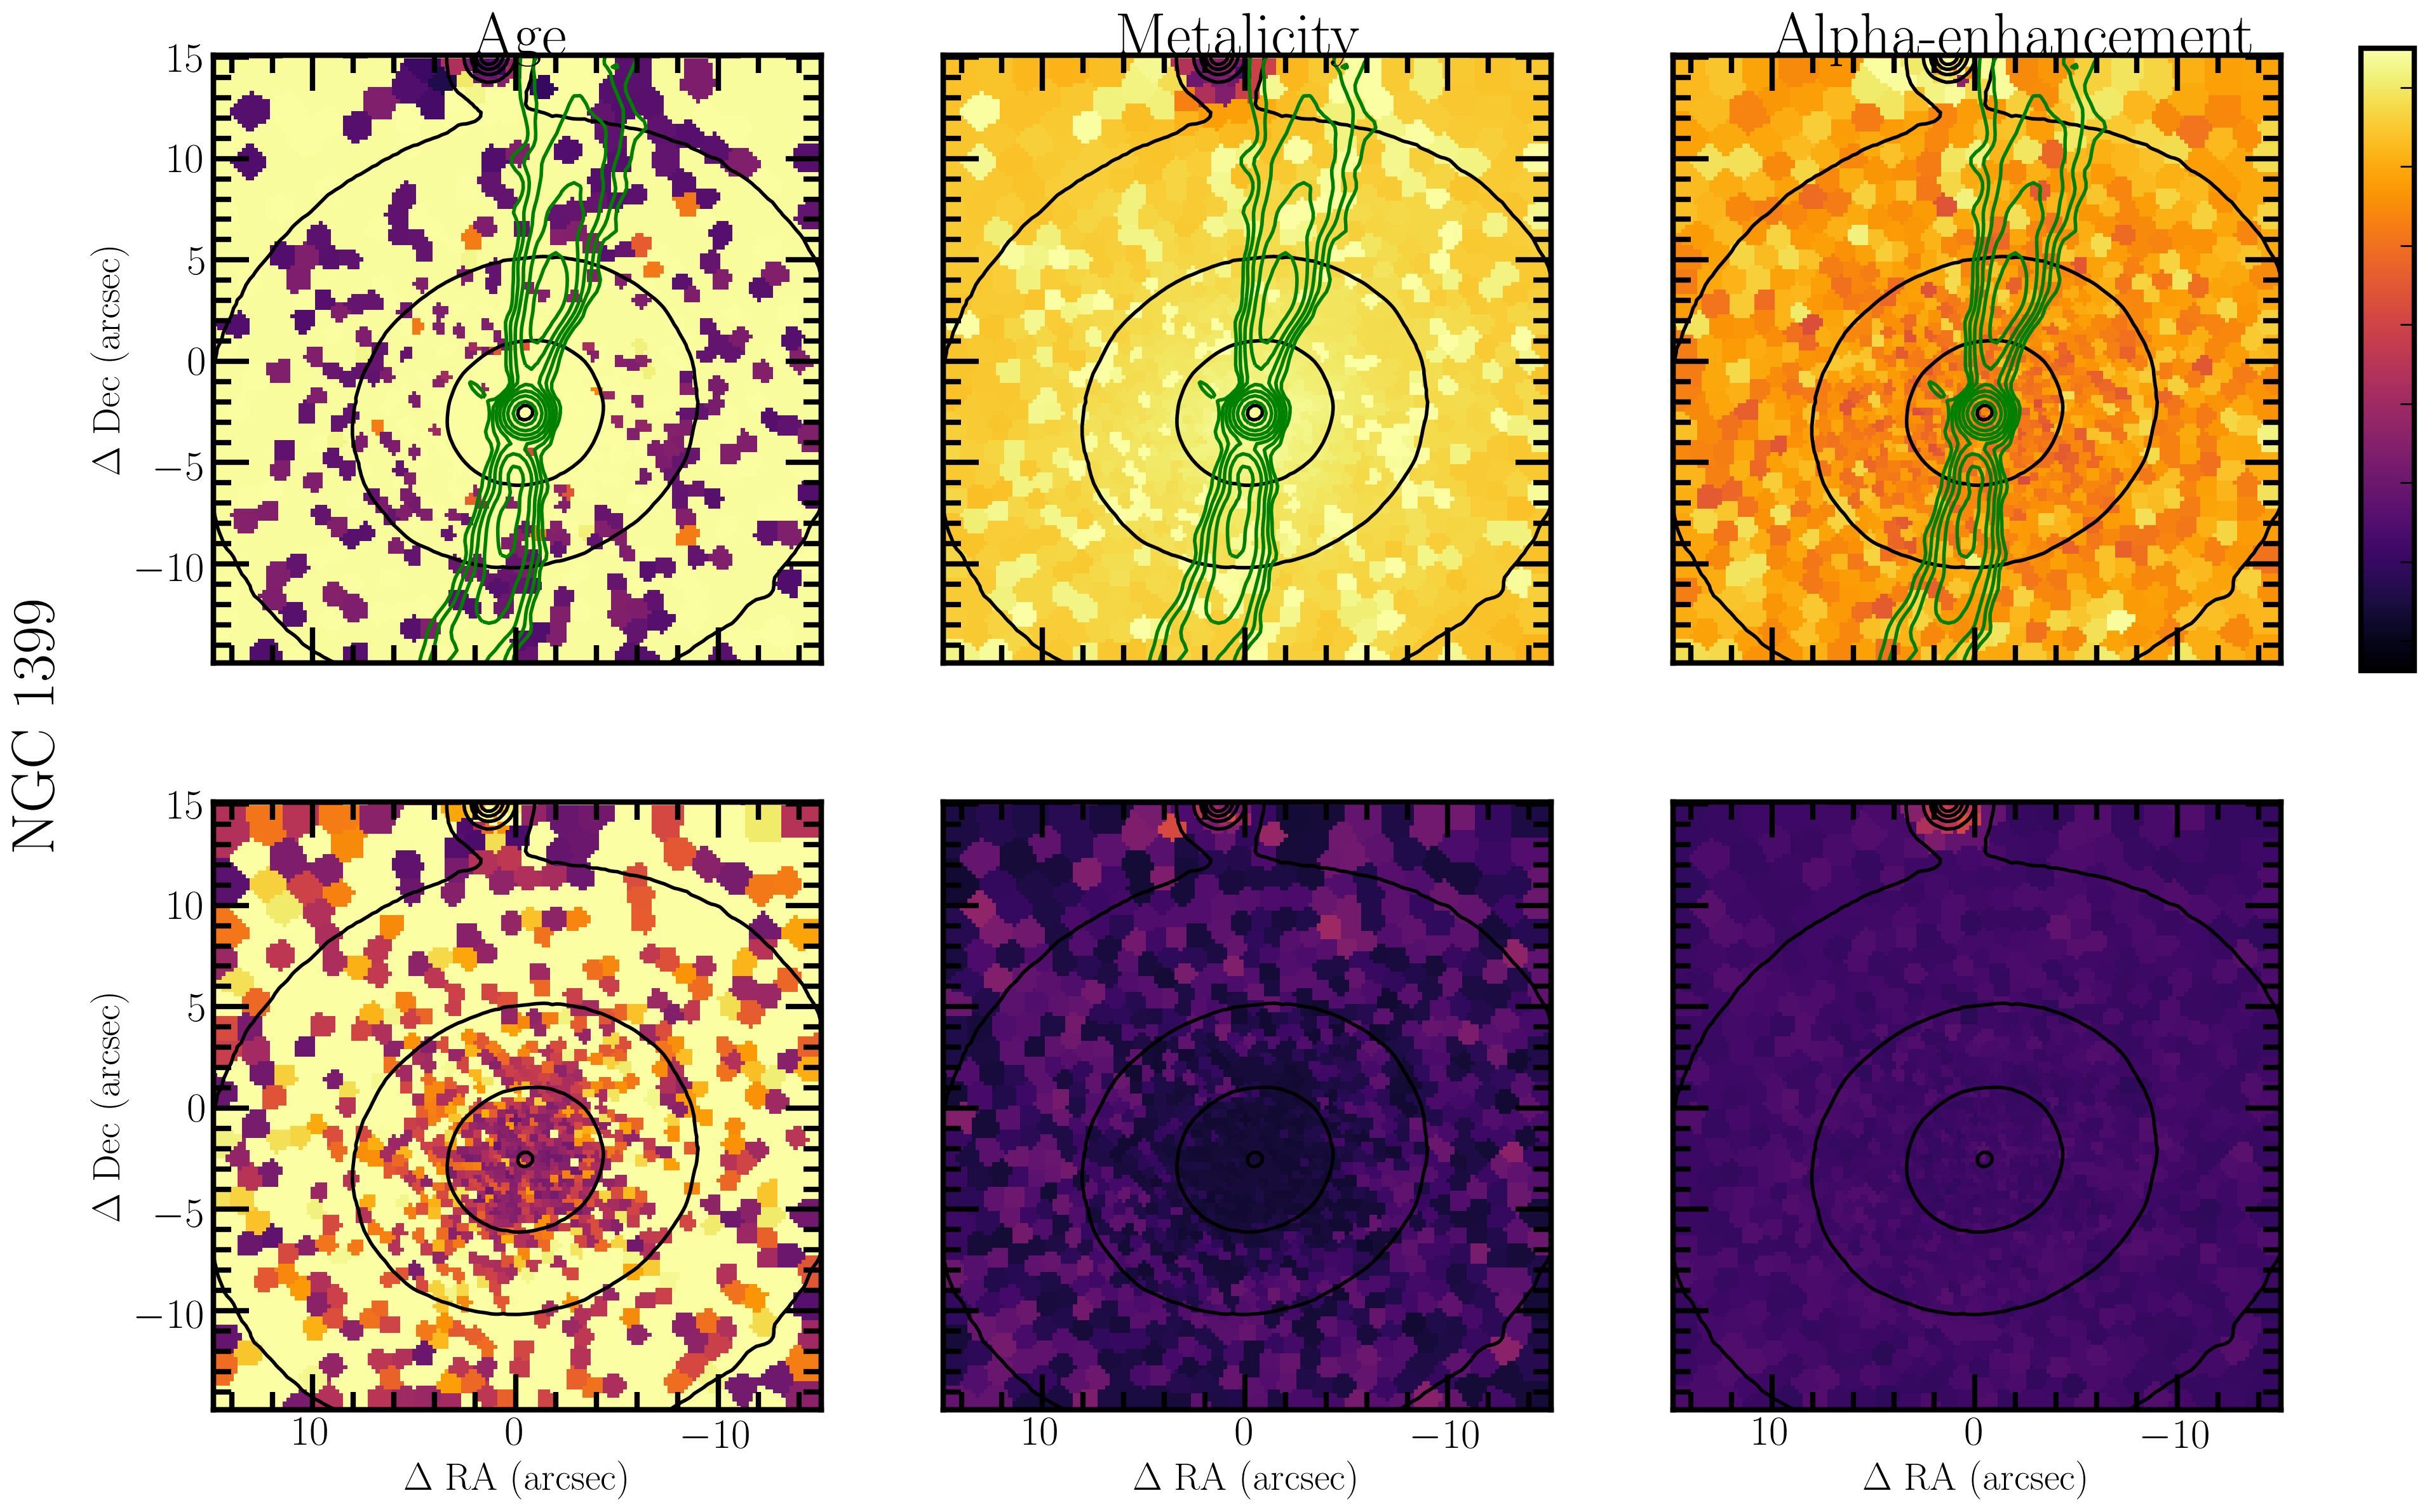
\includegraphics[height=0.31\textheight]{chapter4/muse/pop2.png}
		\contcaption{continued for NGC 1399}
	\end{figure*}


		\subsubsection{Radial Gradients in stellar Populations}
			\label{subsubsec:popGrad}

			\citet{Koleva2011} showed that while the can be a large spread in radial gradients of age and metallicity, the mean is fairly well confined. They assume a linear relationship between $\log \text{age}$ or [Fe/H] and $\log R/R_e$ and for elliptical galaxies they find average gradients of $0.06\pm0.09 \mathrm{log(Gyr) \, arcsec^{-1}$ and $-0.26\pm0.08 \mathrm{[Fe/H]_odot \, arcsec^{-1}$ for the age and metallicity gradients respectively. For S0s they find flatter corresponding gradients of $0.01\pm0.11$ and $-012\pm0.13$. The results from our southern sample are shown in table \ref{tab:popGrad}. We find an average gradients of $-0.004\pm0.003 \mathrm{log(Gyr) \, arcsec^{-1}$ and $-0.025\pm0.002 \mathrm{[Fe/H]_odot \, arcsec^{-1}$ for the age and metallicity gradients respectively, which given the small sample size shows remarkable consistancy with \citet{Koleva2011}.

			\begin{table}
				\centering
				\caption{The radial gradient of the most-likely SSP model for each of the Southern Sample assuming a linear gradient.}
				\label{tab:popGrad}
				\begin{tabular}{l c c}
					\hline
					\hline
					Galaxy 	& $\Delta_\text{log age}$ & $\Delta_\text{[Fe/H]} \\ 
						& log(Gyr) arcsec$^{-1}$ & [Fe/H]$_\odot$ arcsec$^{-1}$ \\
					\hline
					ESO 443-G024 & $-0.008 \pm 0.006$ & $-0.028 \pm 0.005$ \\
					IC 1459 	& $-0.024 \pm 0.011$ & $-0.024 \pm 0.022$ \\
					IC 1531 	& $-0.016 \pm 0.006$ & $0.004 \pm 0.009$ \\
					IC 4296		& $0.001 \pm 0.001$ & $0.071 \pm 0.006$ \\
					NGC 612 	& $0.021 \pm 0.024$ & $-0.101 \pm 0.012$ \\
					NGC 1316 	& $0.007 \pm 0.004$ & $0.005 \pm 0.006$ \\
					NGC 1399 	& $-0.035 \pm 0.008$ & $0.041 \pm 0.006$ \\
					NGC 3100 	& $0.000 \pm 0.004$ & $-0.045 \pm 0.003$ \\
					NGC 3557 	& $0.000 \pm 0.006$ & $-0.023 \pm 0.007$ \\
					NGC 7075 	& $0.006 \pm 0.003$ & $-0.067 \pm 0.006$ \\
					PKS 718-34  & $0.008 \pm 0.007$ & $-0.115 \pm 0.007$ \\
				\end{tabular}
			\end{table}



	\subsection{Kinematically Decoupled Cores}
		\label{sec:popKDC}

		\citet{Kuntschner2010} found that KDCs exist in two forms: they are either small or contain an old stellar population. The three definite KDCs found in the Southern Sample fit into this pattern, all with old stellar populations and varying sizes. It is worth noting that in many cases we would not resolve any of the small KDCs: they would be 1 spaxel in size. Figure \ref{fig:KDC} shows the KDC size -- age relation including the Southern Sample. KDC size is the radius at which $k_1$ goes to zero at the boundary between inner and outer components. Age is the age corresponding to the most-likely model for the inner 1 arcsec. We have included PKS 718-34 in this plot which we stress is only tentatively classified as containing a KDC from the kinematics from VIMOS. Figure \ref{fig:KDC} shows that while it would be an extremely large KDC it would still fit with the findings of \citet{Kuntschner2010}.

		\begin{figure}
			\centering
			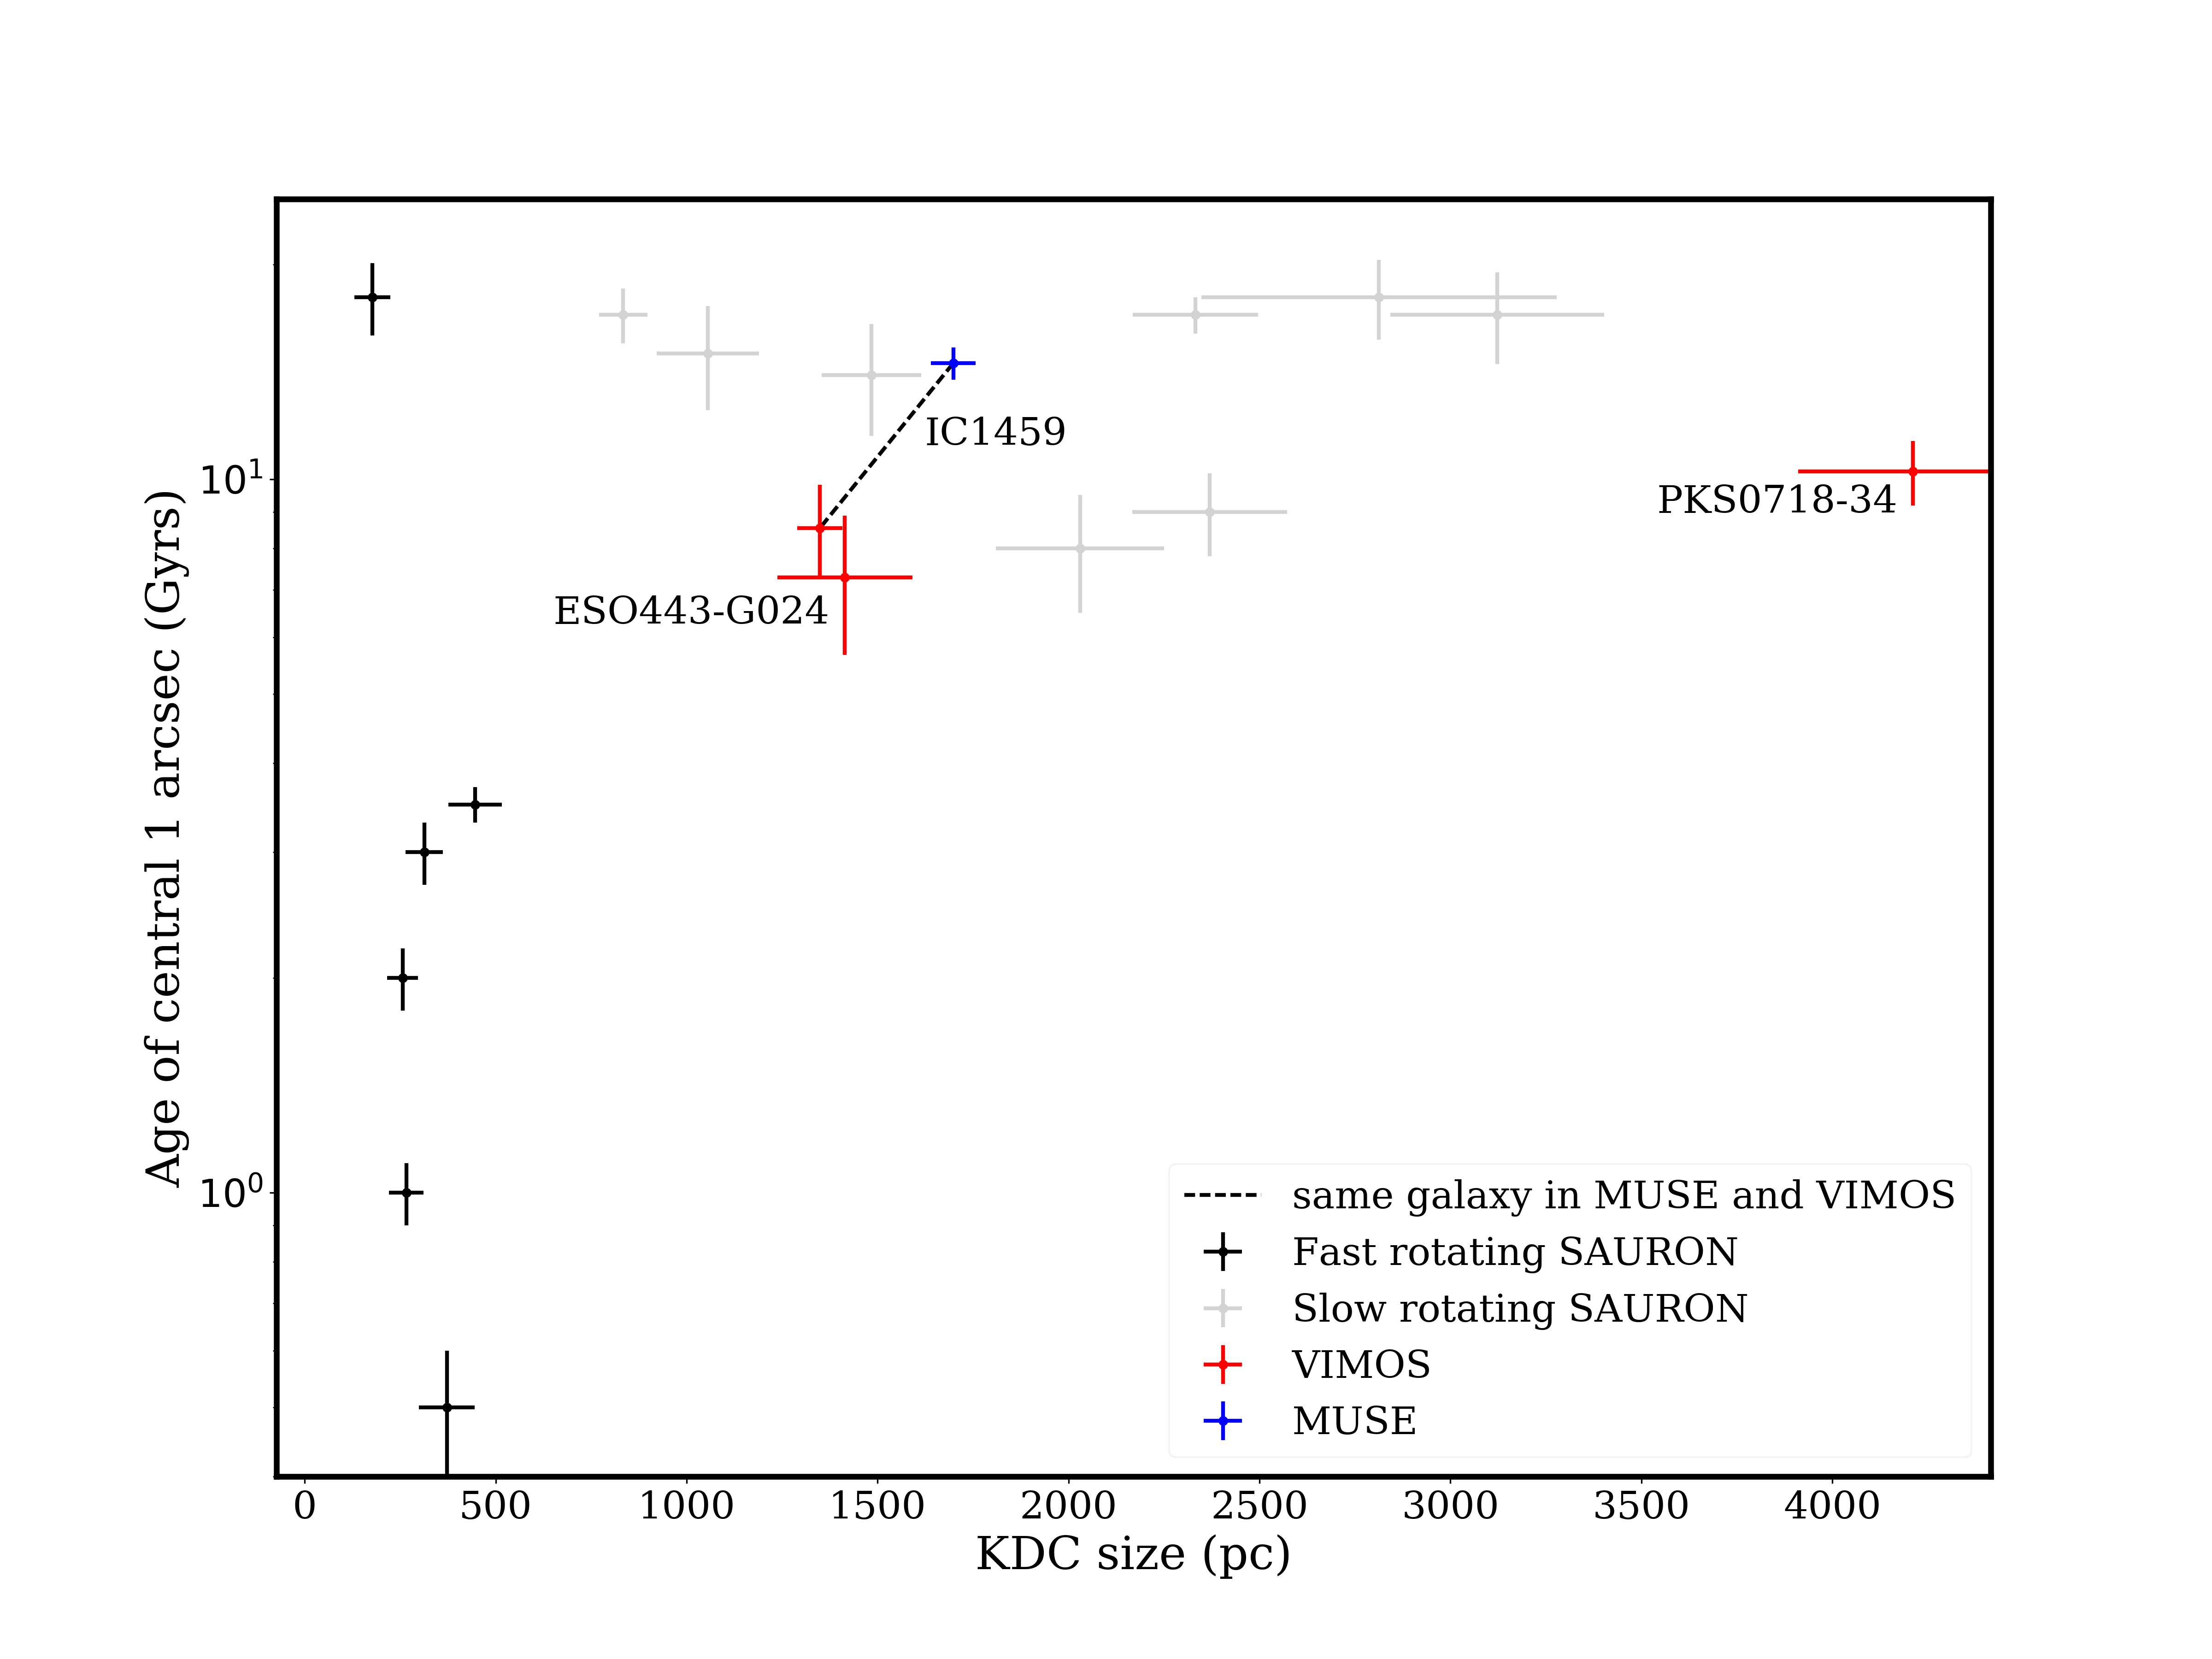
\includegraphics[width=.8\textwidth]{chapter4/KDC_size_age.png}
			\caption[KDC dichotomy]{The KDC size -- age relation showing KDCs are either old or small. Colors of symbols are: VIMOS in red, MUSE in blue and SAURON from \citet{Kuntschner2010} in black and gray for fast and slow rotators respectively (Atlas3D did not repeat these measurements after SAURON.}
			\label{fig:KDC}
		\end{figure}


	\subsection{Mg -- \textsigma relation}
		\label{subsec:Mgsigma}

		It was \citet{Bender1993} who first noticed the unusually tight relationship betweem the global Mg absorption line strength and velocity dispersion for elliptical galaxies. They also noticed that residuals appeared to be intrisic as they had a near gaussian shape about the median values, but did not seem to be correlated to any other galaxy property. Since there is no known process that would correlate these values at late times in the evolution of galaxy, this seems to favour the notion that ETGs had a very short formation epoch at high redshift. 

		\citet{Mehlert2003} showed the existance of the internal Mg--\textsigma relation, but also suggested that it had a different origin to that of the global relation. They found that alpha-enhancement correlates with velocity dispersion and drives about 30\% of the global Mg--\textsigma relation, with metallicity variations providing the remaining 70\%, while the alpha-enhancement usually has no radial gradient (while velocity dispersion is highly correlated to radius) suggesting that alpha-enhancement has no role in the internal Mg--\textsigma relation. 

		\subsubsection{Global relation}
			Using an aperture of 2 arcsec we find a global gradient of $2.7\pm1.9 \mathrm{\AA \, log(km s^{-1})^{-1}}$. This is consistent with the gradient found by \citet{Ziegler1997} for a sample of elliptical galaxies within Virgo and Coma using data from \citet{Dressler1987}, however there is an considerable offset of $\sim0.75\AA$. Figure \ref{fig:globalMg} shows our measurement (which are also given in table \ref{tab:globalMg}) with the bestfitting line (solid line). The result of \citet{Ziegler1997} (eq. 2 in that paper) is also shown as the dashed line. 
			%%no uncertainties quoted in Dressler1987 so comparison is meaningless.
			%NGC 1399 was observed by \citet{Dressler1987}, but measures Mg$_2$ instead of Mg$_b$. In order to compare we make use of the linear conversion (eq. 1 in \citet{Ziegler1997}):
			% \begin{equation}
			% 	\mathrm{Mg_b \, \AA^{-1}} = 15 \mathrm{Mg_2 \, mag^{-1}}
			% \end{equation}
			% Using this gives that \citet{Dressler1987} measured NGC 1399 to have a Mg$_b$ strength of 5.175 and a velocity dispersion of 299.9 km s$^{-1}$, however \citet{Dressler1987} does not quote uncertainties for their values so it is difficult to make comparisons. 

			\begin{table}
				\centering
				\caption{The Mg$_b$ index and velocity dispersion within 2 arcsec. NGC 612 and PKS 718-34 have a redshift which shifts the Mg$_b$ feature outside of the wavelength range of VIMOS.}
				\label{tab:globalMg}
				\begin{tabular}{l c c}
					\hline
					\hline
					Galaxy 	& Mg$_b$ & $\sigma$ \\
							& \AA 	& km s$^{-1}$ \\
					\hline
					ESO 443-G024 & $4.43 \pm 0.08$ & $332.4 \pm 1.6$ \\
					IC 1459 	& $4.67 \pm 0.03$ & $292.7 \pm 0.6$ \\
					IC 1531 	& $3.74 \pm 0.06$ & $222.9 \pm 1.3$ \\
					IC 4296		& $4.57 \pm 0.13$ & $361.7 \pm 2.1$ \\
					NGC 612 	& --   			  & $228.5 \pm 1.9$ \\
					NGC 1316 	& $3.45 \pm 0.08$ & $233.3 \pm 1.5$ \\
					NGC 1399 	& $4.57 \pm 0.13$ & $319.1 \pm 2.1$ \\
					NGC 3100 	& $4.36 \pm 0.05$ & $214.2 \pm 1.1$ \\
					NGC 3557 	& $4.15 \pm 0.03$ & $280.4 \pm 0.9$ \\
					NGC 7075 	& $4.45 \pm 0.07$ & $258.7 \pm 1.9$ \\
					PKS 718-34  & -- 		      & $258.7 \pm 1.9$ \\
					\hline \\
				\end{tabular}
			\end{table}

			\begin{figure}
				\centering
				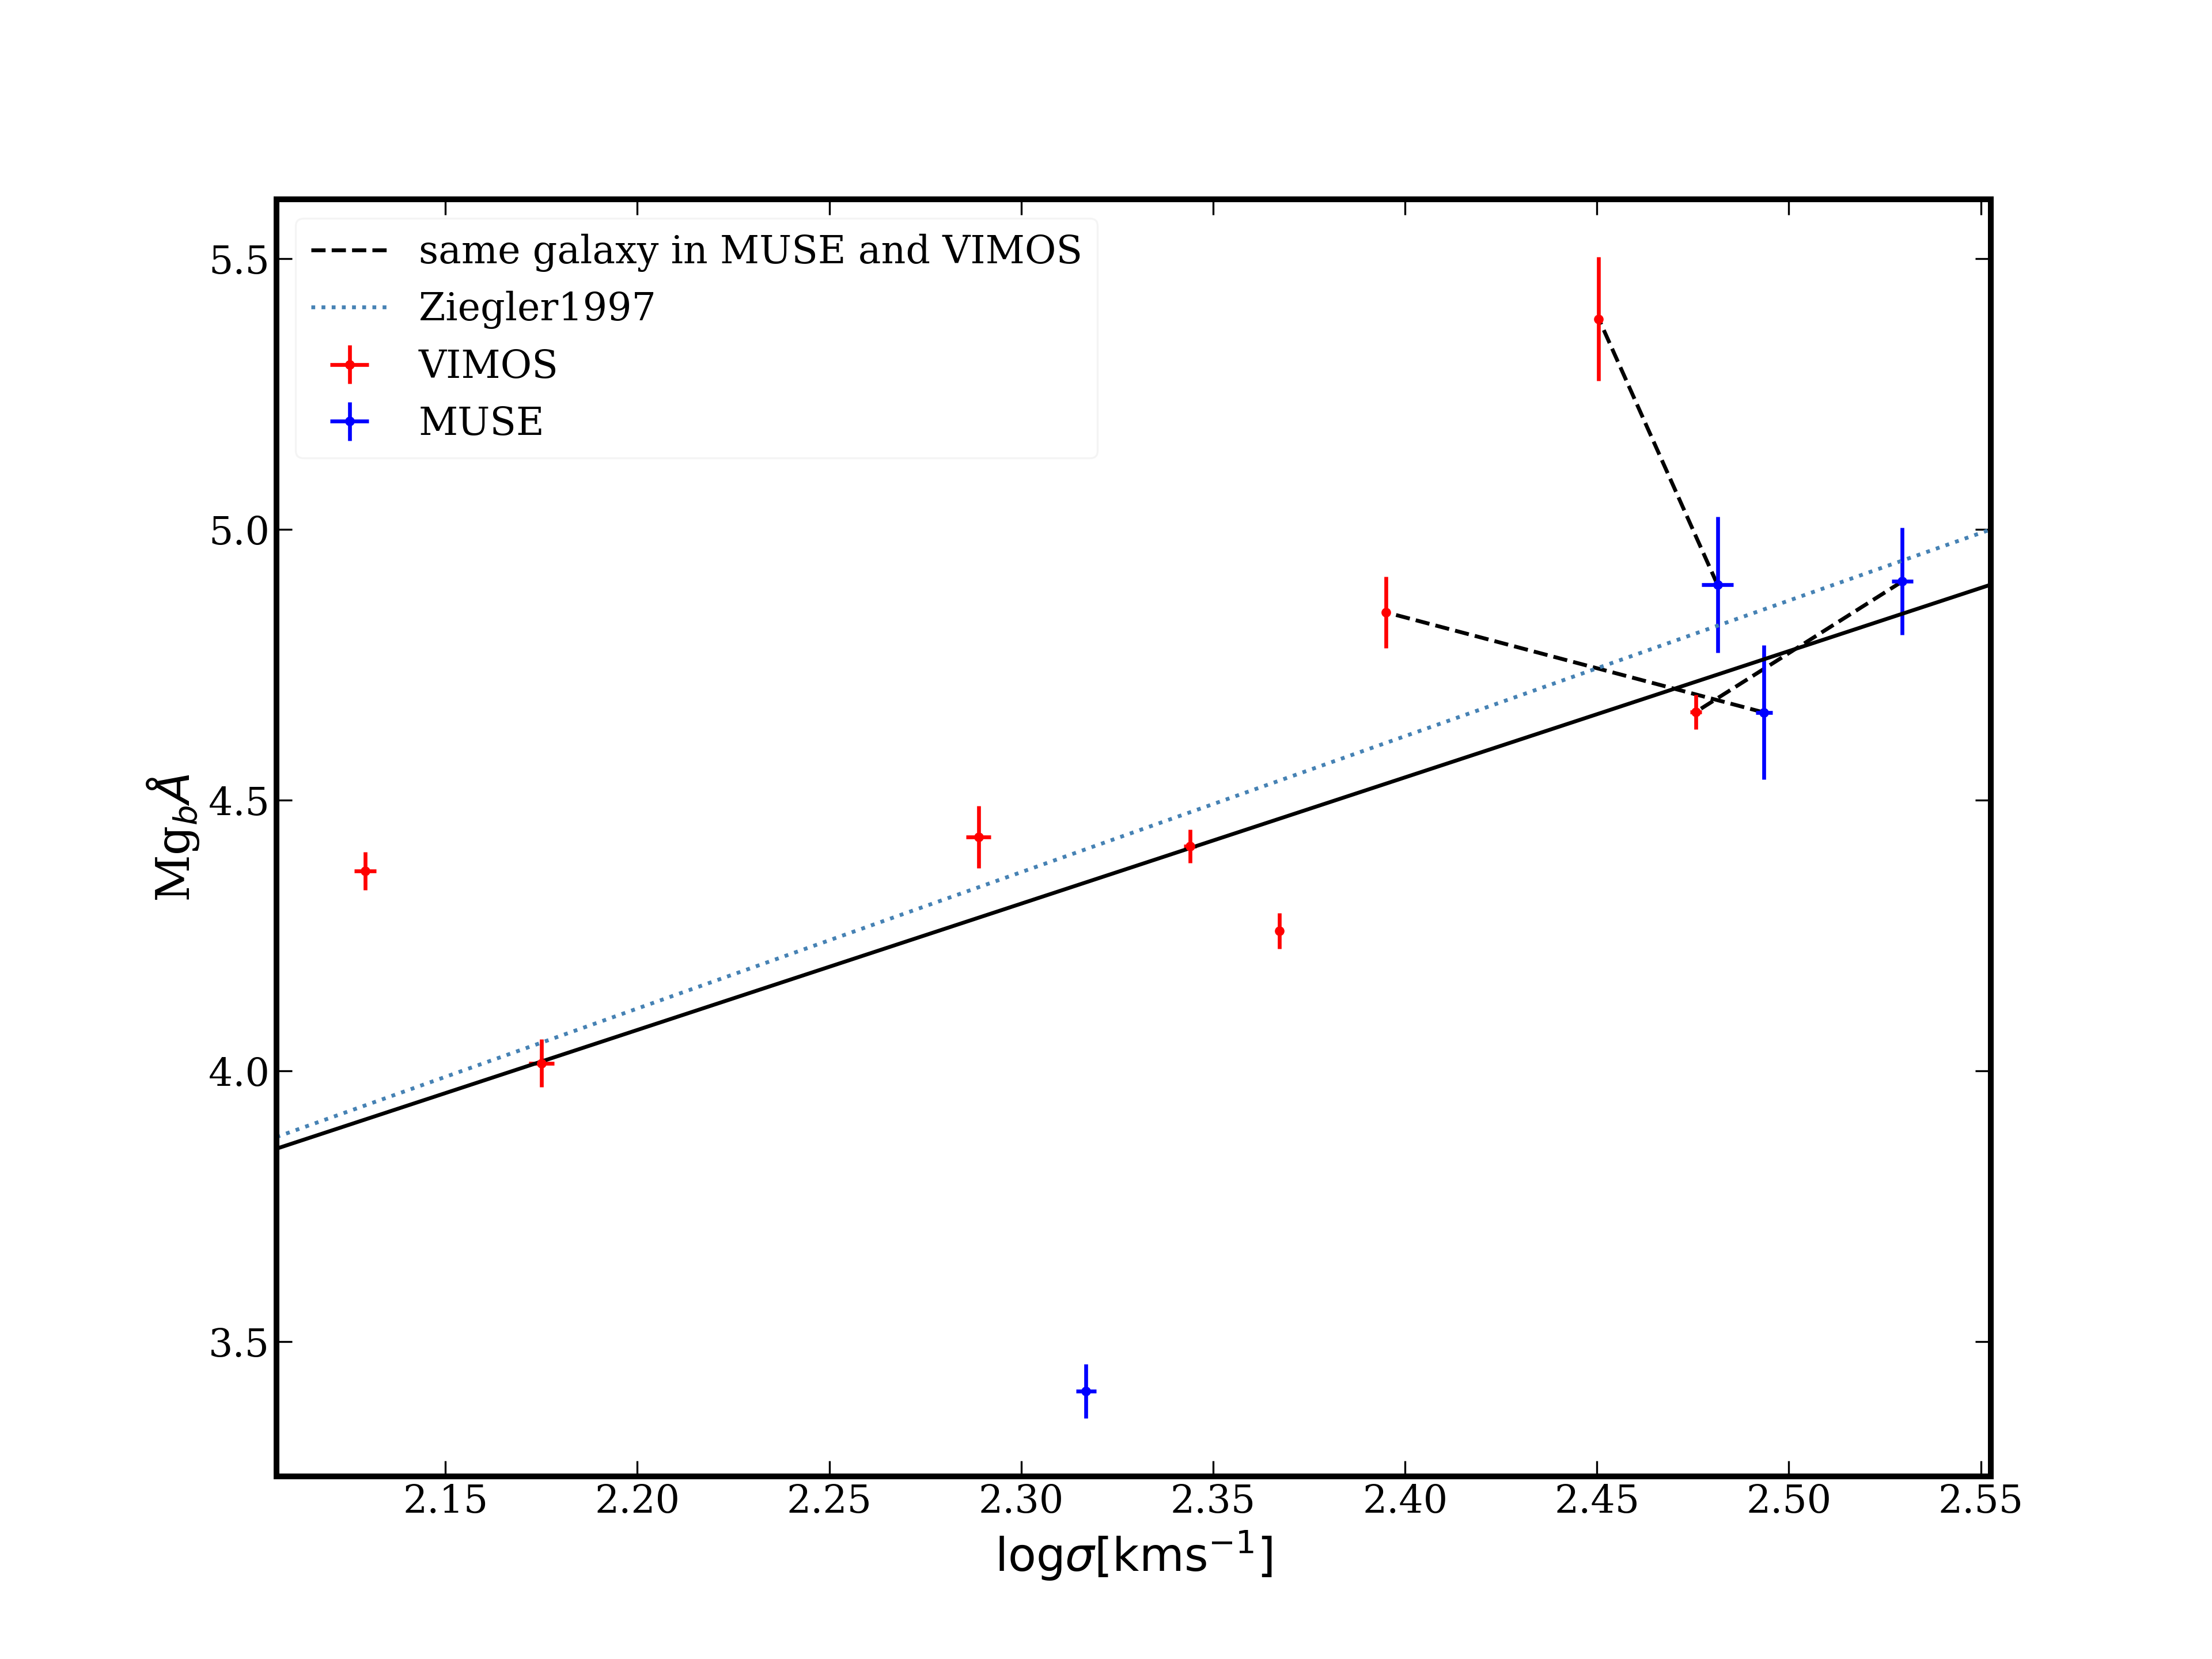
\includegraphics[width=.8\textwidth]{chapter4/Mg_sigma.png}
				\caption[Global Mg$_b$--\textsigma]{The Mg$_b$ -- velocity dispersion relation using a 2" aperture.}
				\label{fig:globalMg}
			\end{figure}

		\subsubsection{Spatially resolved}

\section{The case of NGC 612}
	\label{sec:NGC612}
	All of the galaxies show typical ETG behavior: old, metal rich stellar populations with dispersion dominated stellar kinematics; with the exception of NGC 612. This galaxy has very high rotational velocities for an ETG, with an extended CO disk and a young stellar population. All this suggests that NGC 612 must have a very different history to the rest of the Southern Sample. Indeed, the CO and ionized gas disks are more representative of LTGs, rather than ETGs. With this in mind, we tentatively suggest that NGC 612 may be a very edge-on spiral galaxy and not intrinsically an ETG at all. Having said that, it is worth noting that spiral galaxies with radio jets, particularly on the scale of NGC 612's jets are very rare with only a handful of known cases \citep{}. 
	%Certainly a strong case for reclassifying as LTG